\RequirePackage{flashmovie}

\documentclass[aspectratio=169, xcolor=table]{beamer}
\usepackage{etex}
\usepackage{booktabs}
\usepackage{amsmath,amsfonts}
\usepackage{graphicx}
\usepackage{subfigure,pdfpages}
\usepackage{wrapfig}
% \usepackage[3D]{movie15}
% \usepackage{movie15}
\usepackage[american]{babel}
\usepackage{tablefootnote}
\usepackage[T1]{fontenc}
\usepackage{listings}
\usepackage{lmodern}
\usepackage{textcomp}
\usepackage{chngcntr}


\usetheme{Goddard}



\newcommand{\filepath}{\texttt}
\newcommand{\command}{\texttt}
\newcommand{\email}[1]{\href{mailto:#1}{\texttt{#1}}}
\newcommand{\latexcode}{\texttt}
\newcommand{\parameter}[1]{\textlangle #1\textrangle}


\lstset{basicstyle=\ttfamily,keywordstyle=\color{goddardblue}\bfseries,commentstyle=\color{goddardblue!75}\itshape,columns=flexible}

\rowcolors{1}{goddardblue!50}{goddardblue!30}

\title[Weekly Presentation]{Weekly Presentation}
\author[{Mohammad}]{{\textbf{By:}\\\vspace{0.2cm} Mohammad Sharifzadeh\\
\vspace{0.3cm}
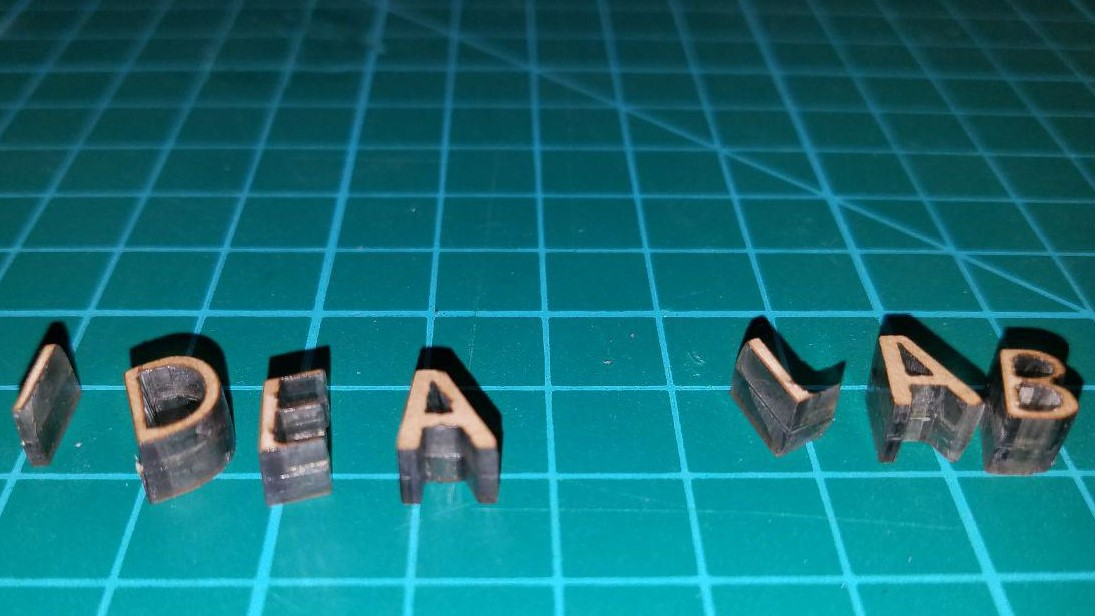
\includegraphics[height=2.7cm]{Idea_Pic}}}

\beamertemplatenavigationsymbolsempty

%----------------------------------------------------------------------
%----------------------------------------------------------------------
%----------------------------------------------------------------------
%----------------------------------------------------------------------
%----------------------------------------------------------------------

\begin{document}

\begin{frame}
  \titlepage
\end{frame}

% ----------------------- Report of 26 May -------------------------
% ----------------------- Report of 26 May -------------------------
% ----------------------- Report of 26 May -------------------------


\part{Report of 26 May 2017}
%\frame{\partpage}
% \section{What's Done?}

% \begin{frame}{Still on the 1st Paper}
% \begin{block}{What we have done so far:}
% \begin{itemize}
% \item Pynamics code is being optimized and ready\\
% \textcolor{blue} {Thanks to Dan \& Roozbeh :-)}
% \item I'm working on hinge characterization\\
% Stiffness \& Damping (Material \& Air)
% \item Designed and modeled a simple hinge
% \end{itemize}
% \end{block}

% \begin{block}{Single Pendulum model:}
% \begin{equation*}
% (I_G + m r^2) \ddot{\theta} = -mg\text{sin}\theta - k\theta - c\dot{\theta}
% \end{equation*}
% \begin{center}
% \small
% $k$: Stiffness\\
% $c$: Overall damping: Material \& Air\\
% $r$: Distance between center of mass and center of orientation\\
% \normalsize
% \end{center}
% \end{block}
% \end{frame}

% \begin{frame}{Hinge Characterization}
% \begin{block}{Getting experimental data}
% \begin{itemize}
% \item Get data by using tracking camera
% \item Needs filtering before differentiation\\ 
% Numerical filtering changed the data\\ 
% \hspace{2cm} $\Downarrow$ $\Downarrow$ $\Downarrow$ \\
% $\Rightarrow$ First fit "Fourier Series to data"\\
% $\Rightarrow$ Then apply analytic filtering
% \end{itemize}
% \begin{center}
% 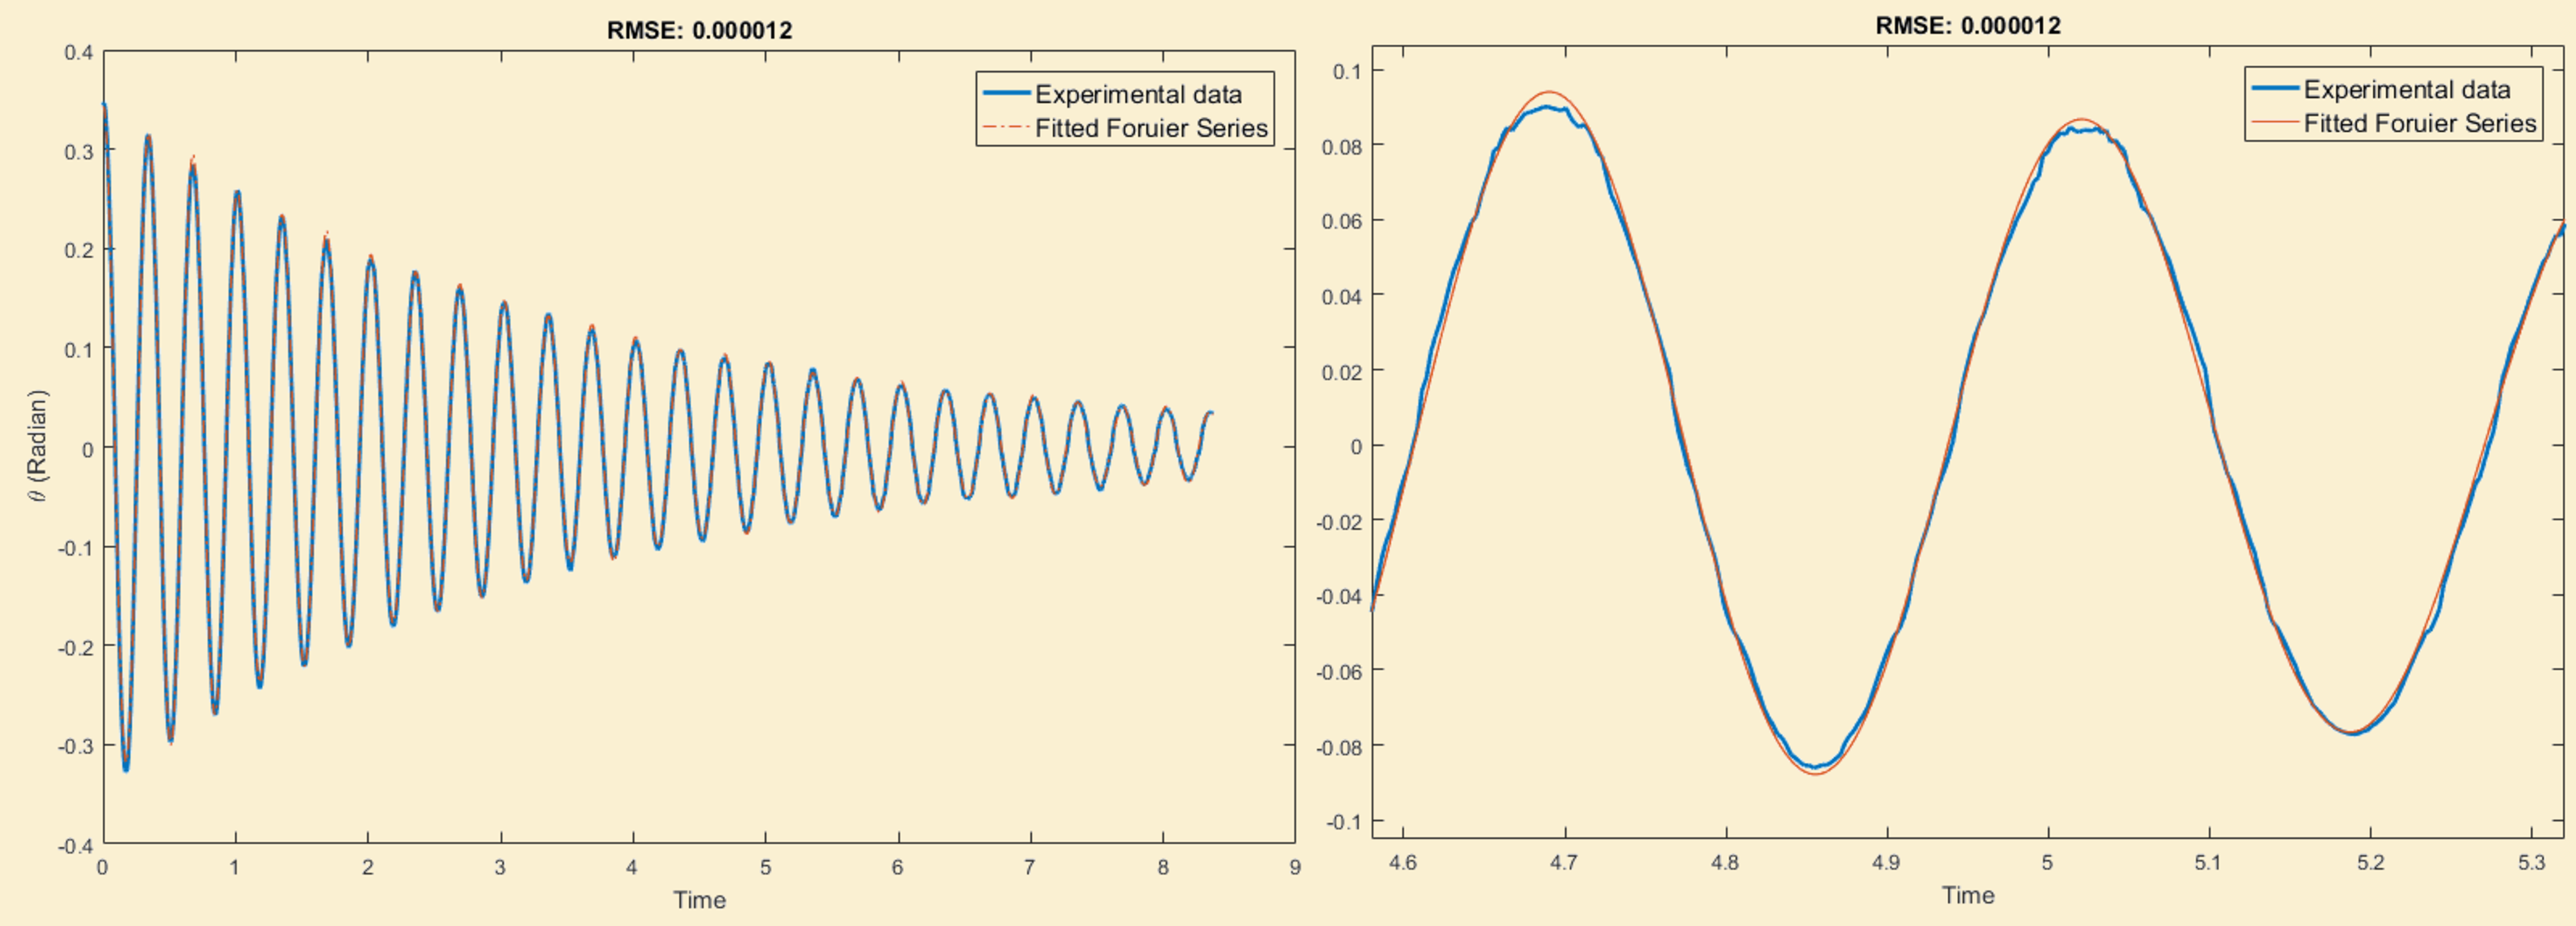
\includegraphics[scale=0.16]{FS_Fit.pdf}
% \end{center}
% \end{block}
% \end{frame}


% \begin{frame}{Hinge Characterization}
% \begin{block}{Identification process}
% \begin{itemize}
% \item Rewrite the model:
% \begin{equation*}
% (I_G + m r^2) \ddot{\theta} + mg\text{sin}\theta = - k\theta - c\dot{\theta}
% \end{equation*}
% \item The left part is known based on experimental and PopupCAD data
% \item Used Least Squares to find "K" and "c"
% \quad \textbf{Least Square:}
% \Large
% \begin{equation*}
% \hat{a} ={(X^T X)}^{-1} X^TY
% \end{equation*}
% \normalsize
% \begin{equation*}
% \hat{a} = [k\quad c] , \quad X = [\theta\quad \dot{\theta}]
% \end{equation*}
% \begin{equation*}
% Y = (I_G + m r^2) \ddot{\theta} + mg\text{sin}\theta
% \end{equation*}
% \end{itemize}
% \end{block}
% \end{frame}


% \section{What's being done?}
% \subsection{Air damping consideration}


% \begin{frame}{Hinge Characterization}
% \begin{block}{Why should consider the air damping?}
% \begin{itemize}
% \item It effects the behavior of the system
% \item It effects the overall damping 
% \item Some do experiments in Vacuum Chambers
% \item Extract \textbf{material damping} from overall damping
% \end{itemize}
% \end{block}
% \begin{block}{What we are suggesting?}
% \begin{itemize}
% \item Use different shapes of body when using a same hinge
% \item Identify the overall damping 
% \item Find a model to fit the different damping caused by the different cross-sections (A) of bodies
% \item Use the offset (A=0) to find the material damping
% \end{itemize}
% \end{block}
% \end{frame}

% \begin{frame}{Hinge Characterization}
% \begin{block}{Why switched to Acrylic?}
% There is so many noise caused by environments (Specially room fans) \hspace{1cm} $\Downarrow$ $\Downarrow$ $\Downarrow$ \\
% Increase the mass $\Rightarrow$ Reduce the acceleration caused by environment $\Rightarrow$ Have less noisy data 
% \end{block}
% \begin{block}{Finally...}
% \begin{center}
% 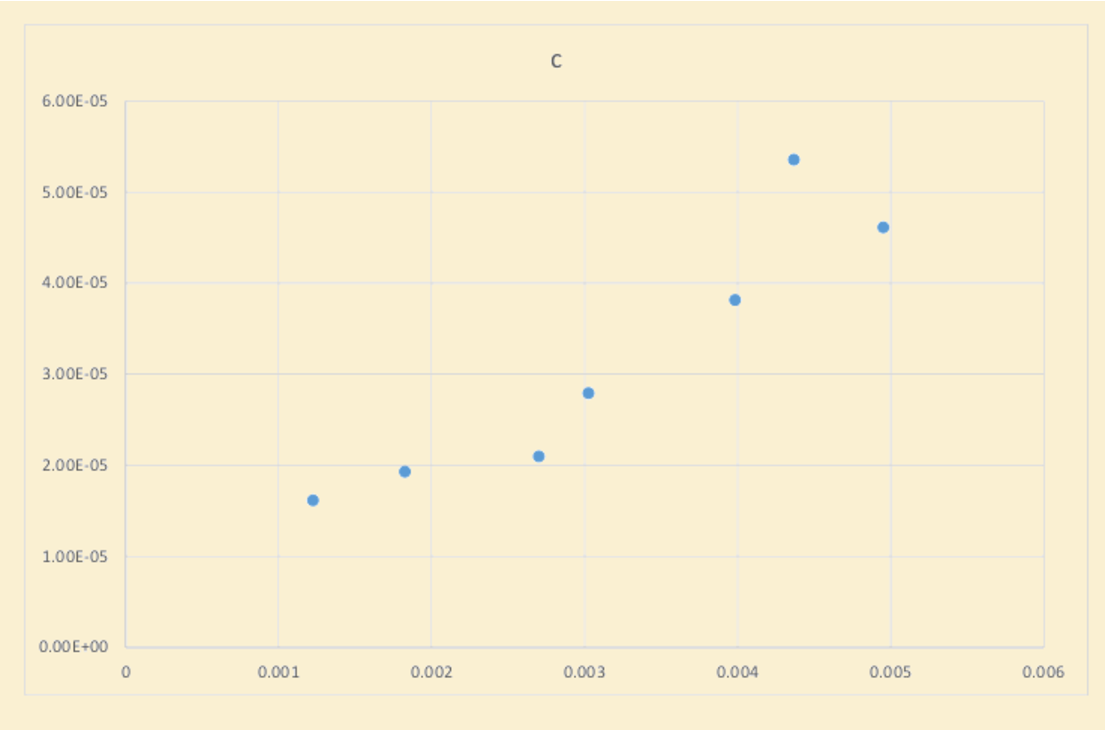
\includegraphics[scale=0.30]{air_d.pdf}
% \end{center}
% \end{block}
% \end{frame}

% \subsection{Different Hinges}

% \begin{frame}{Now it's time for different hinges}
% \begin{block}{Different hinges (Length \& Width)}
% It requires time and material to re-build prototypes by using Acrylics! \hspace{2cm} $\Downarrow$ $\Downarrow$ $\Downarrow$ \\
% \quad\textbf{I want to make it modular!!!}
% \begin{itemize}
% \item Enable us to change the body and hinges independently
% \item Will be useful in all future devices, when the flex layer changes its characteristics
% \end{itemize}
% \end{block}
% \end{frame}

% \subsection{Let's make in modular}

% \begin{frame}{Modular simple hinge}
% \begin{block}{What I'm proposing:}
% \begin{center}
% 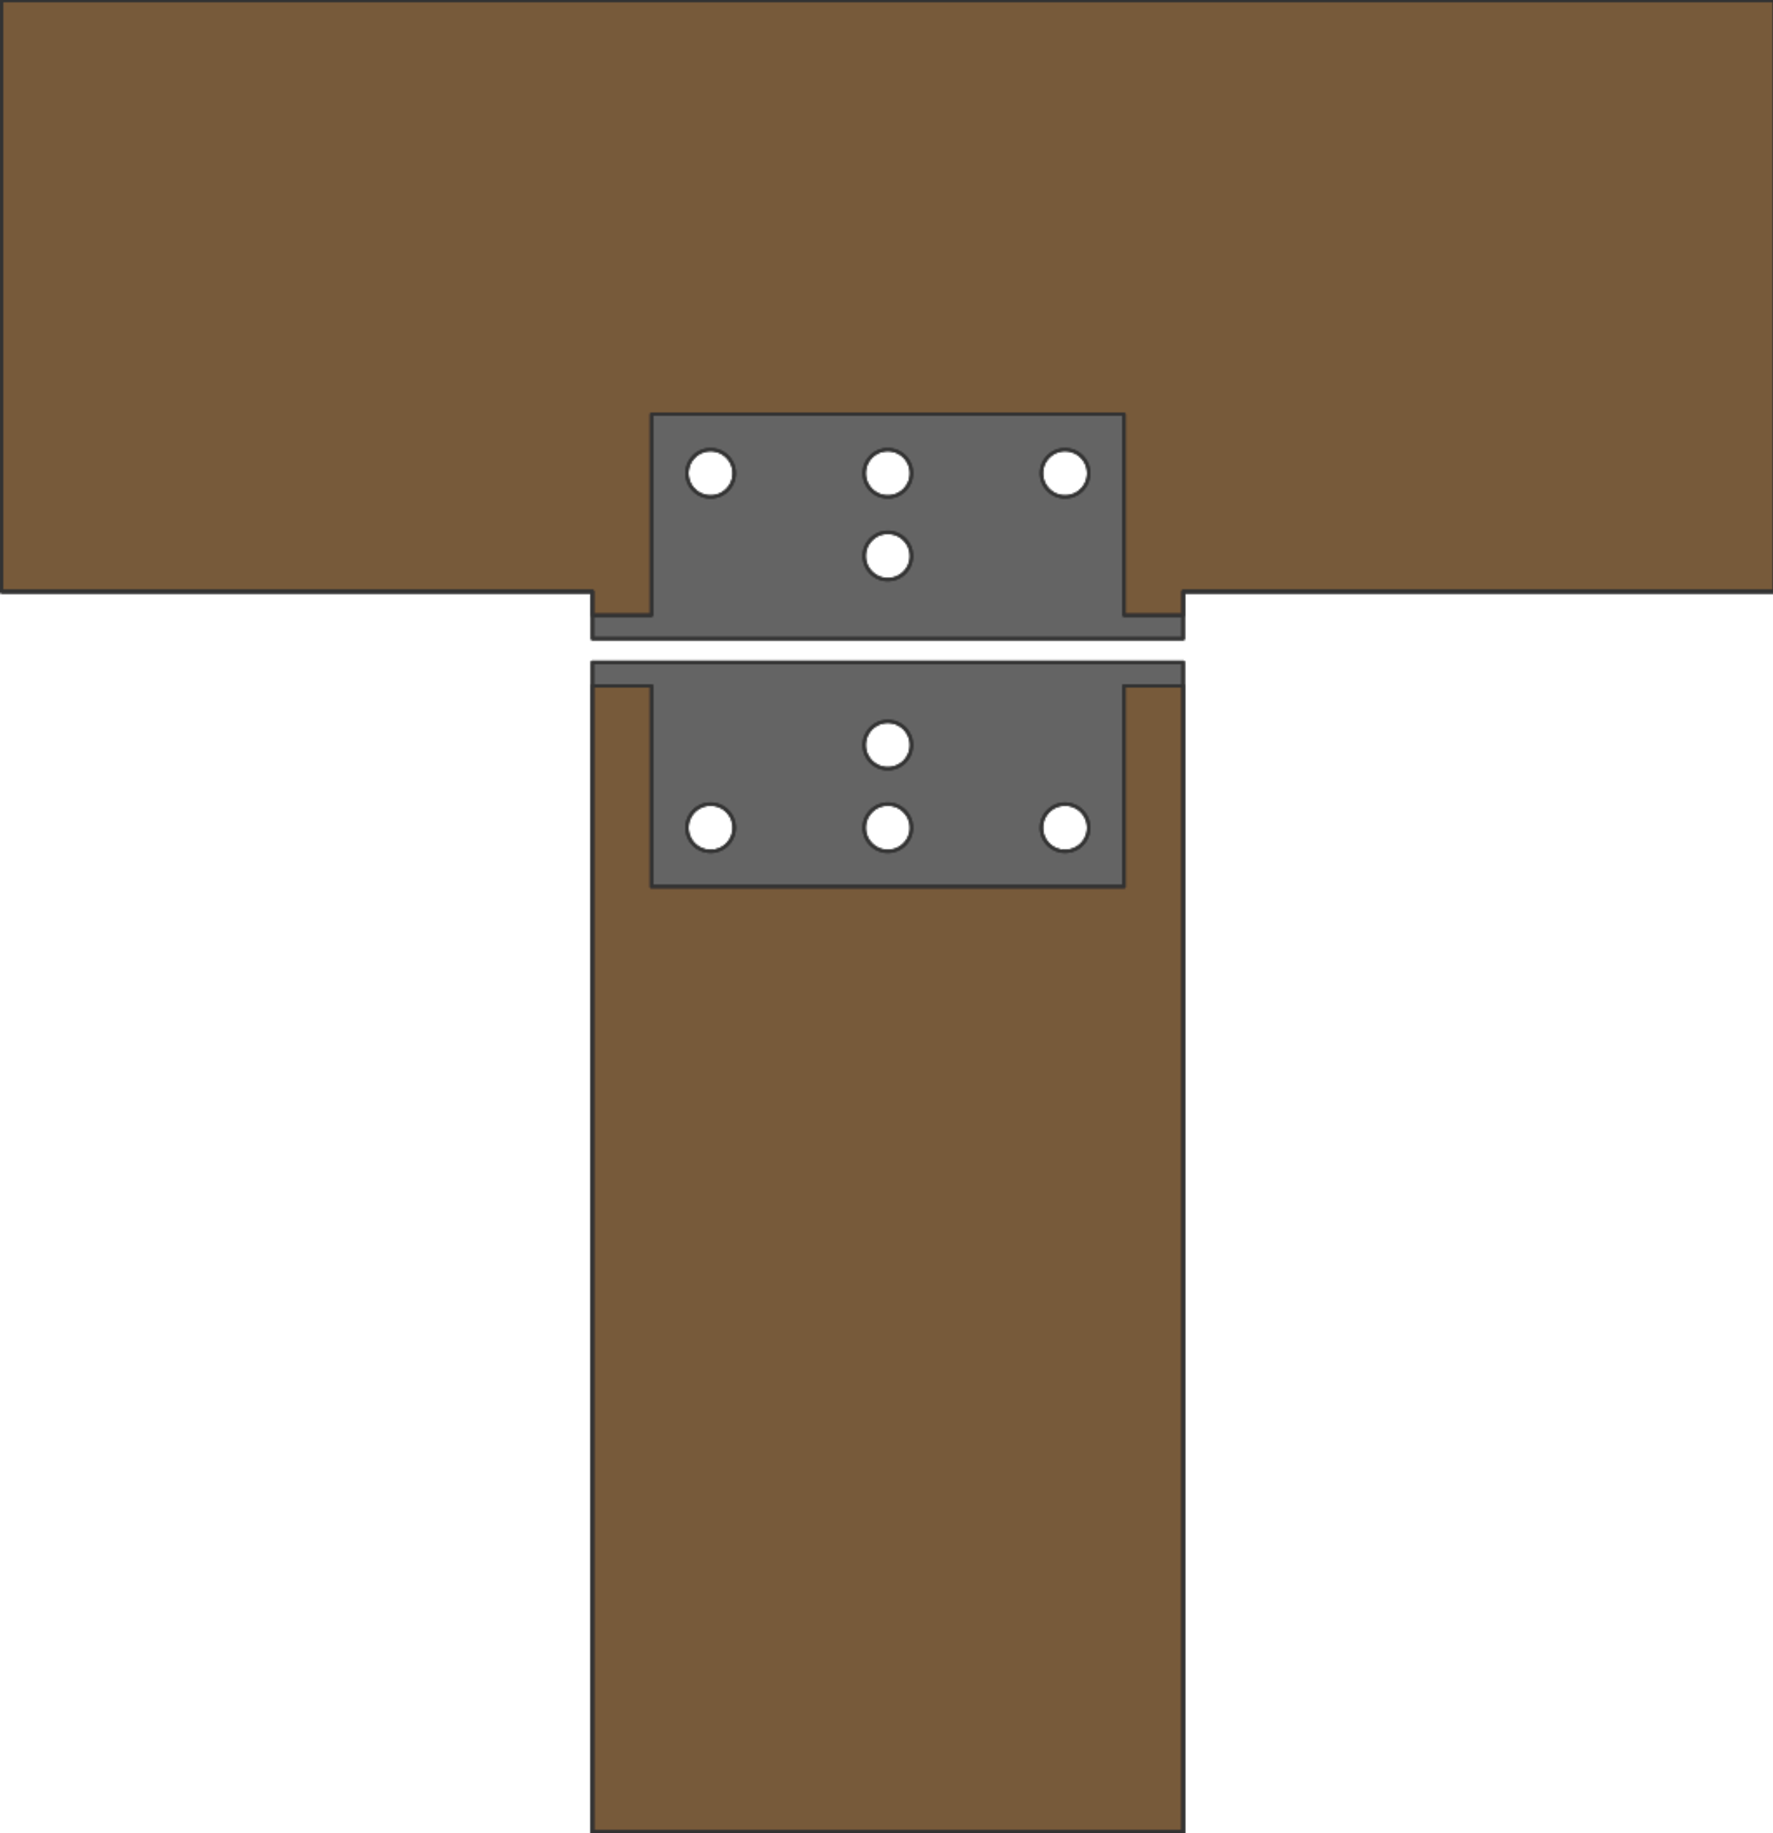
\includegraphics[scale=0.2]{all.pdf}
% \end{center}
% \end{block}
% \end{frame}

% \begin{frame}{Modular simple hinge}
% \begin{block}{What I'm proposing:}
% \begin{center}
% 
\includegraphics[scale=0.2]{2Layer.pdf}
% \end{center}
% \end{block}
% \end{frame}

% \begin{frame}{Modular simple hinge}
% \begin{block}{What I'm proposing:}
% \begin{center}
% \textbf{Now you just need to change design of}\\
% \textbf{the hinge in the flex layer} \\ \vspace{1cm}
% 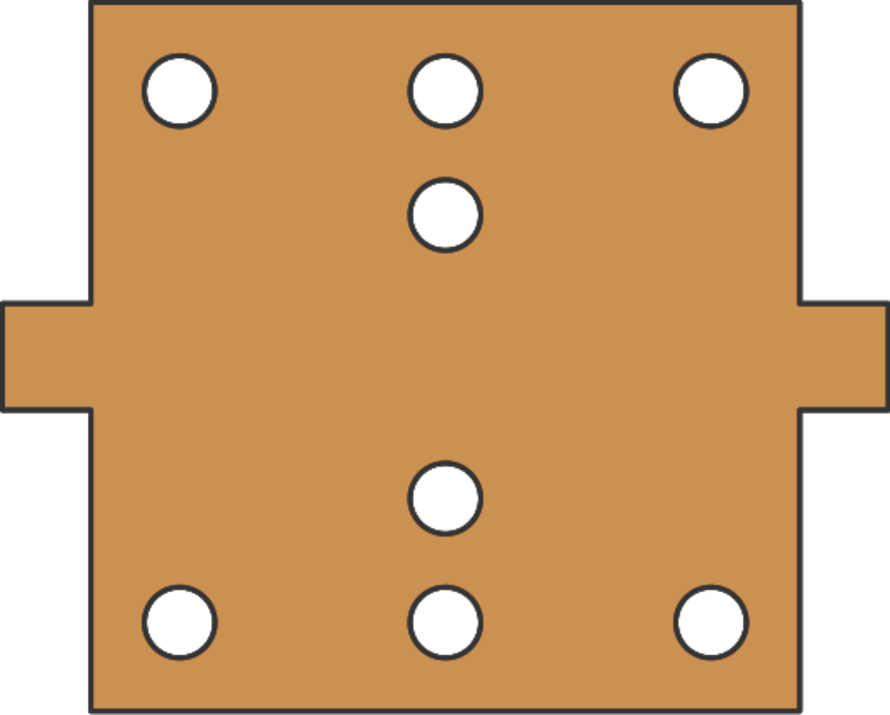
\includegraphics[scale=0.25]{hinge.pdf}
% \end{center}
% \end{block}
% \end{frame}

% ----------------------- Report of 13 June -------------------------
% ----------------------- Report of 13 June -------------------------

\part{Report of 13 June 2017}
% \frame{\partpage}

% \section{What's Done?}
% \begin{frame}{Review Papers}
% \begin{block}{Papers that have Hinge characterizations covered:}
% \begin{itemize}
% %\item Model Driven Design for Flexure-Based Microrobots
% \item \href{run:C:/Users/Mohammad/Google Drive/My read papers/1st Presentation Papers/Doshi.pdf}{Model Driven Design for Flexure-Based Microrobots}
% \vspace{1cm}
% \item \href{run:C:/Users/Mohammad/Google Drive/My read papers/1st Presentation Papers/Bowen.pdf}{Design, Fabrication, and Modeling of an Electro-Magnetic Self-Folding Sheet}
% %\item Design, Fabrication, and Modeling of an Electro-Magnetic Self-Folding Sheet
% \end{itemize}
% \end{block}
% \end{frame}

% \begin{frame}{Still on the Pynamics Paper}
% \begin{block}{What we have done so far:}
% \begin{itemize}
% \item Pynamics code is being optimized and ready\\
% \textcolor{blue} {Thanks to Dan \& Roozbeh :-)}
% \item Designed and modeled a simple hinge
% \item I'm finished with hinge characterization Stiffness \& Damping (Material \& Air)
% \end{itemize}
% \end{block}

% \begin{block}{Single Pendulum model:}
% \begin{equation*}
% (I_G + m r^2) \ddot{\theta} = -mg\text{sin}\theta - k\theta - c\dot{\theta}
% \end{equation*}
% \begin{center}
% \small
% $k$: Stiffness\\
% $c$: Overall damping: Material \& Air\\
% $r$: Distance between center of mass and center of orientation\\
% \normalsize
% \end{center}
% \end{block}
% \end{frame}


% \begin{frame}{Hinge Characterization}
% \begin{block}{The model}
% \begin{center}
% 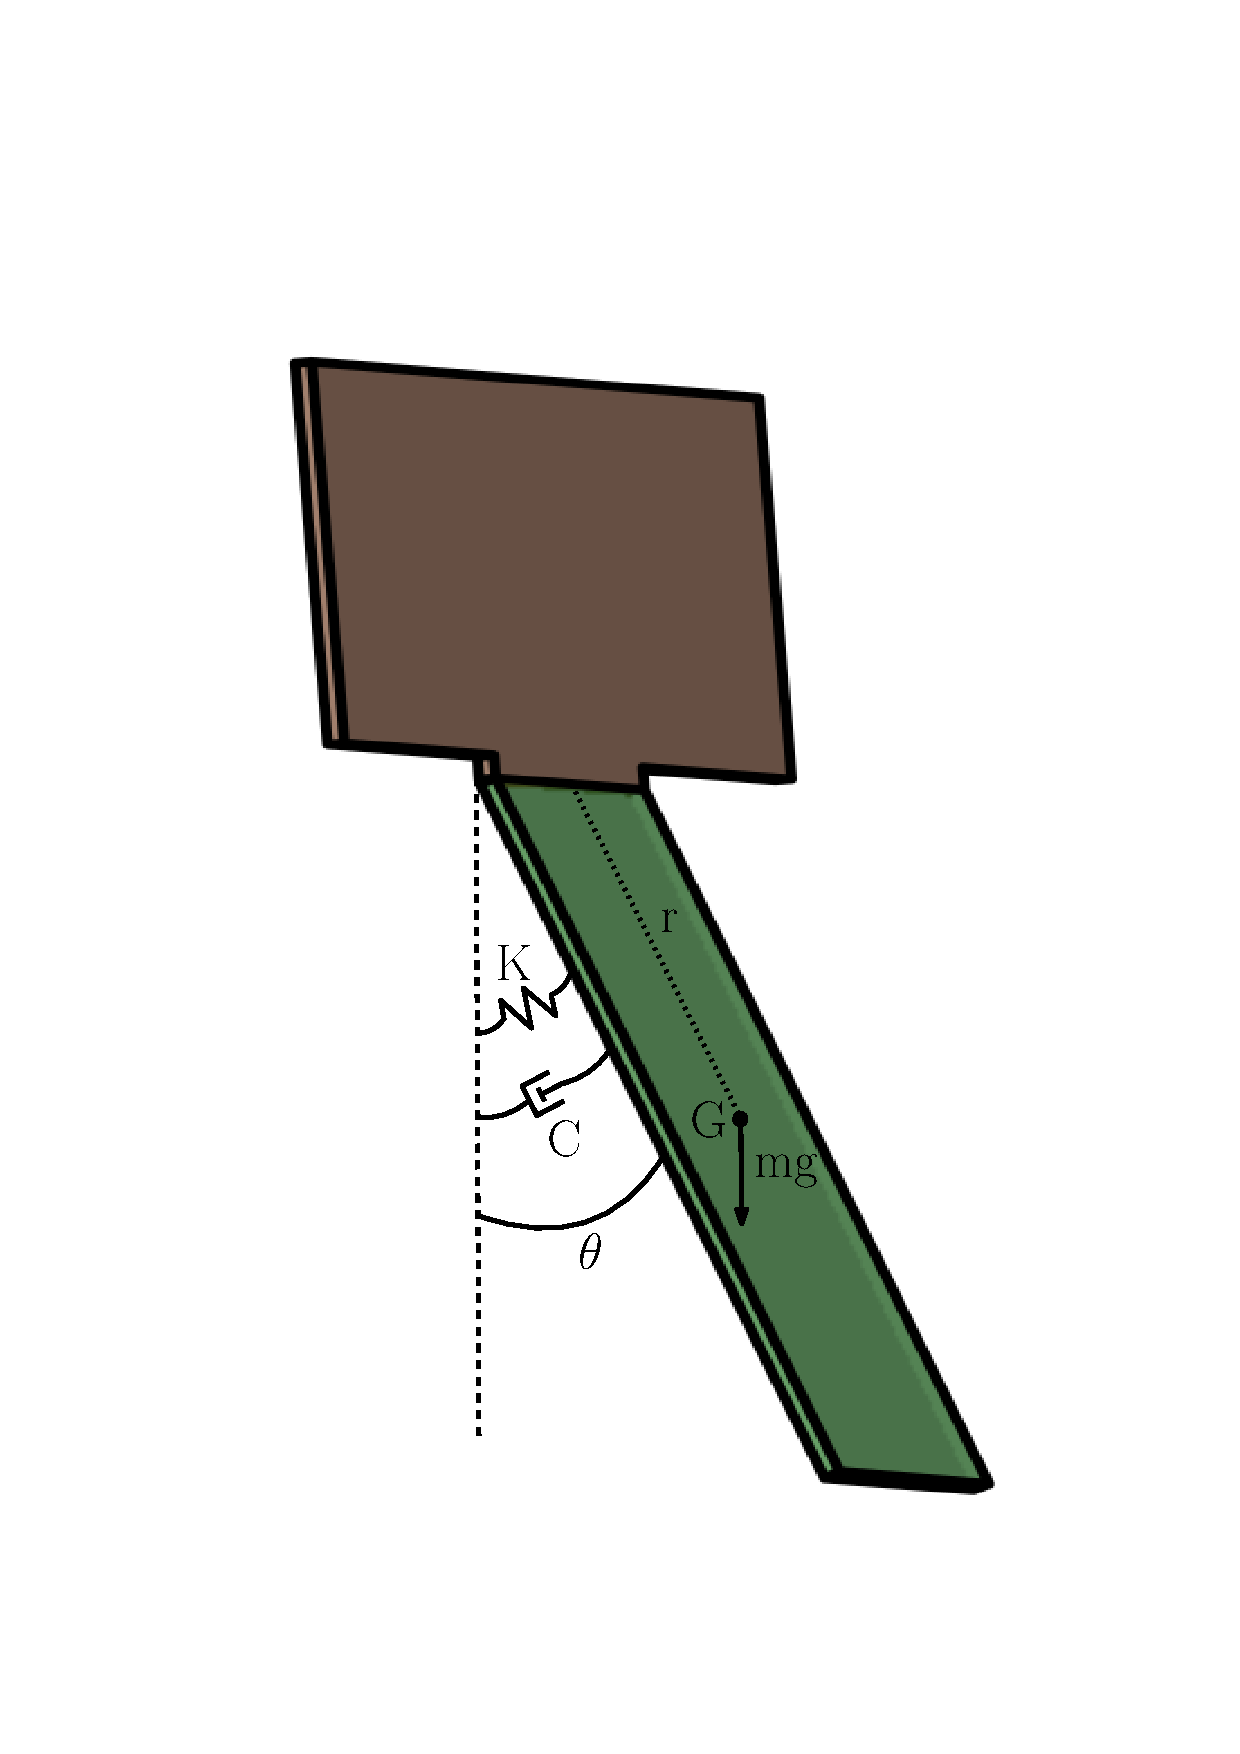
\includegraphics[width=4.5cm]{Model_Pic.pdf}
% \end{center}
% \end{block}
% \end{frame}

% \begin{frame}{Hinge Characterization}
% \begin{block}{Verification using Pynamics}
% \begin{center}
% 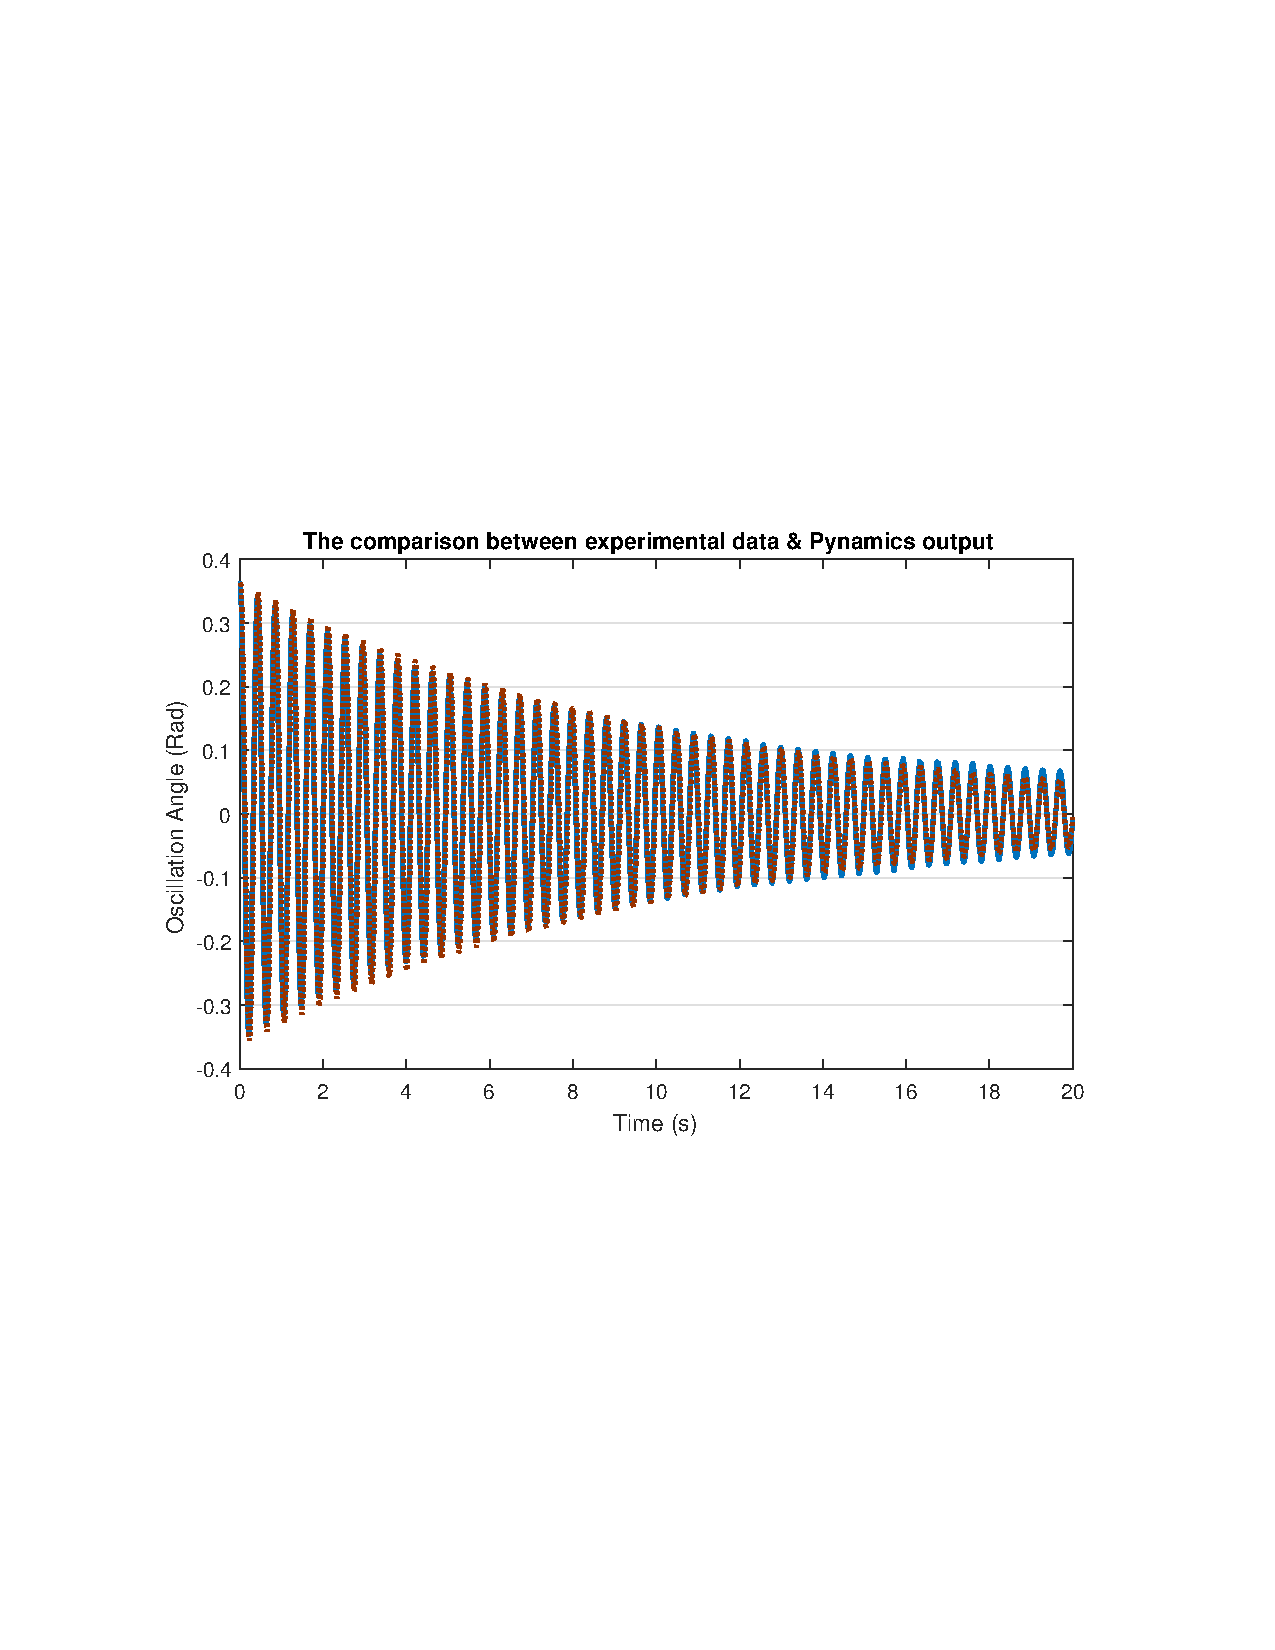
\includegraphics[width=6.5cm]{Case1_Output.pdf}
% \end{center}
% \end{block}
% $\bullet$ Only 2 was not good $\bullet$ All the others fit properly\\ $\bullet$  More than $20\%$ fit amazingly
% \end{frame}

% \subsection{Air damping consideration}
% \begin{frame}{Hinge Characterization}
% \begin{block}{What's effect of air-damping on damping coefficient?}
% \begin{center}
% 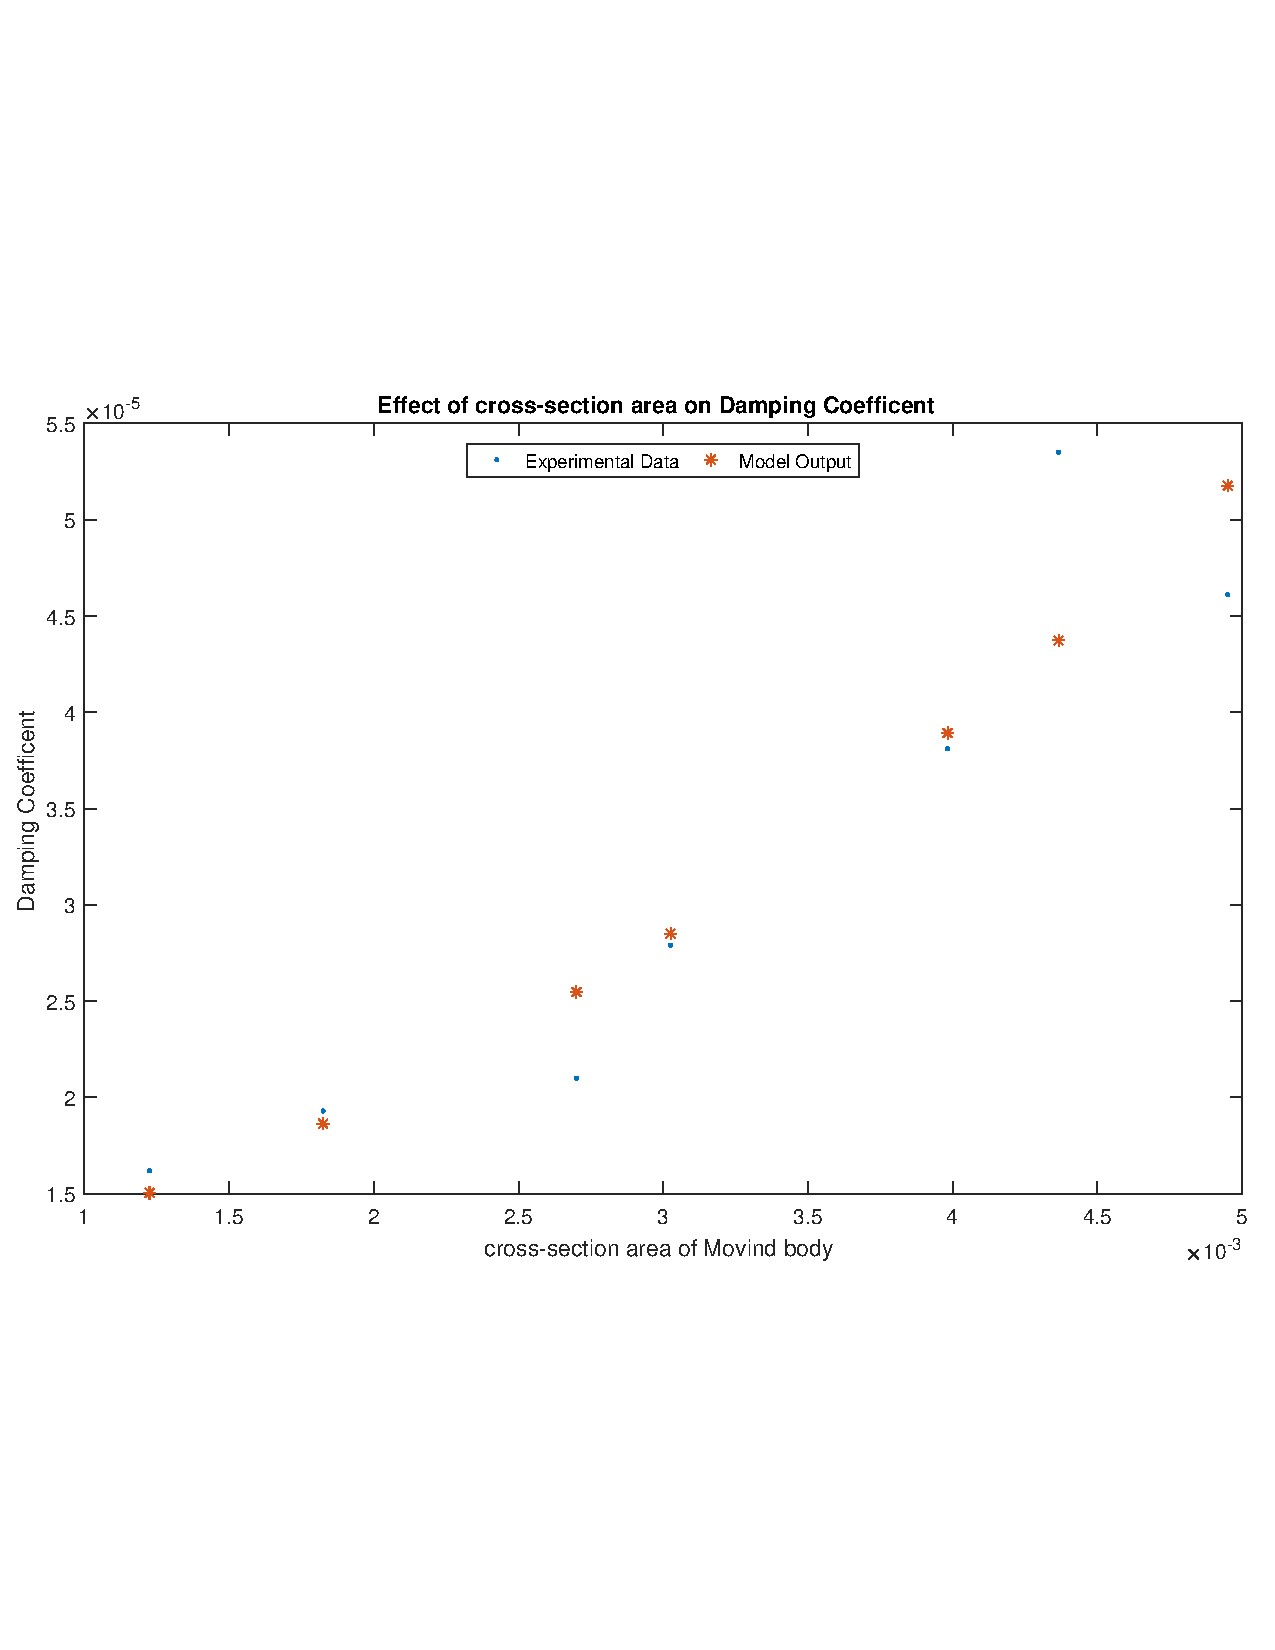
\includegraphics[width=6.5cm]{A_On_C.pdf}
% \end{center}
% \end{block}
% \begin{equation*}
% C = 0.0022 A + 1.2379 A^2 + 1.0484e-05
% \end{equation*}
% \end{frame}

% \subsection{Hinge width consideration}
% \begin{frame}{Hinge Characterization}
% \begin{block}{What's effect of change in width on damping coefficient?}
% \begin{center}
% 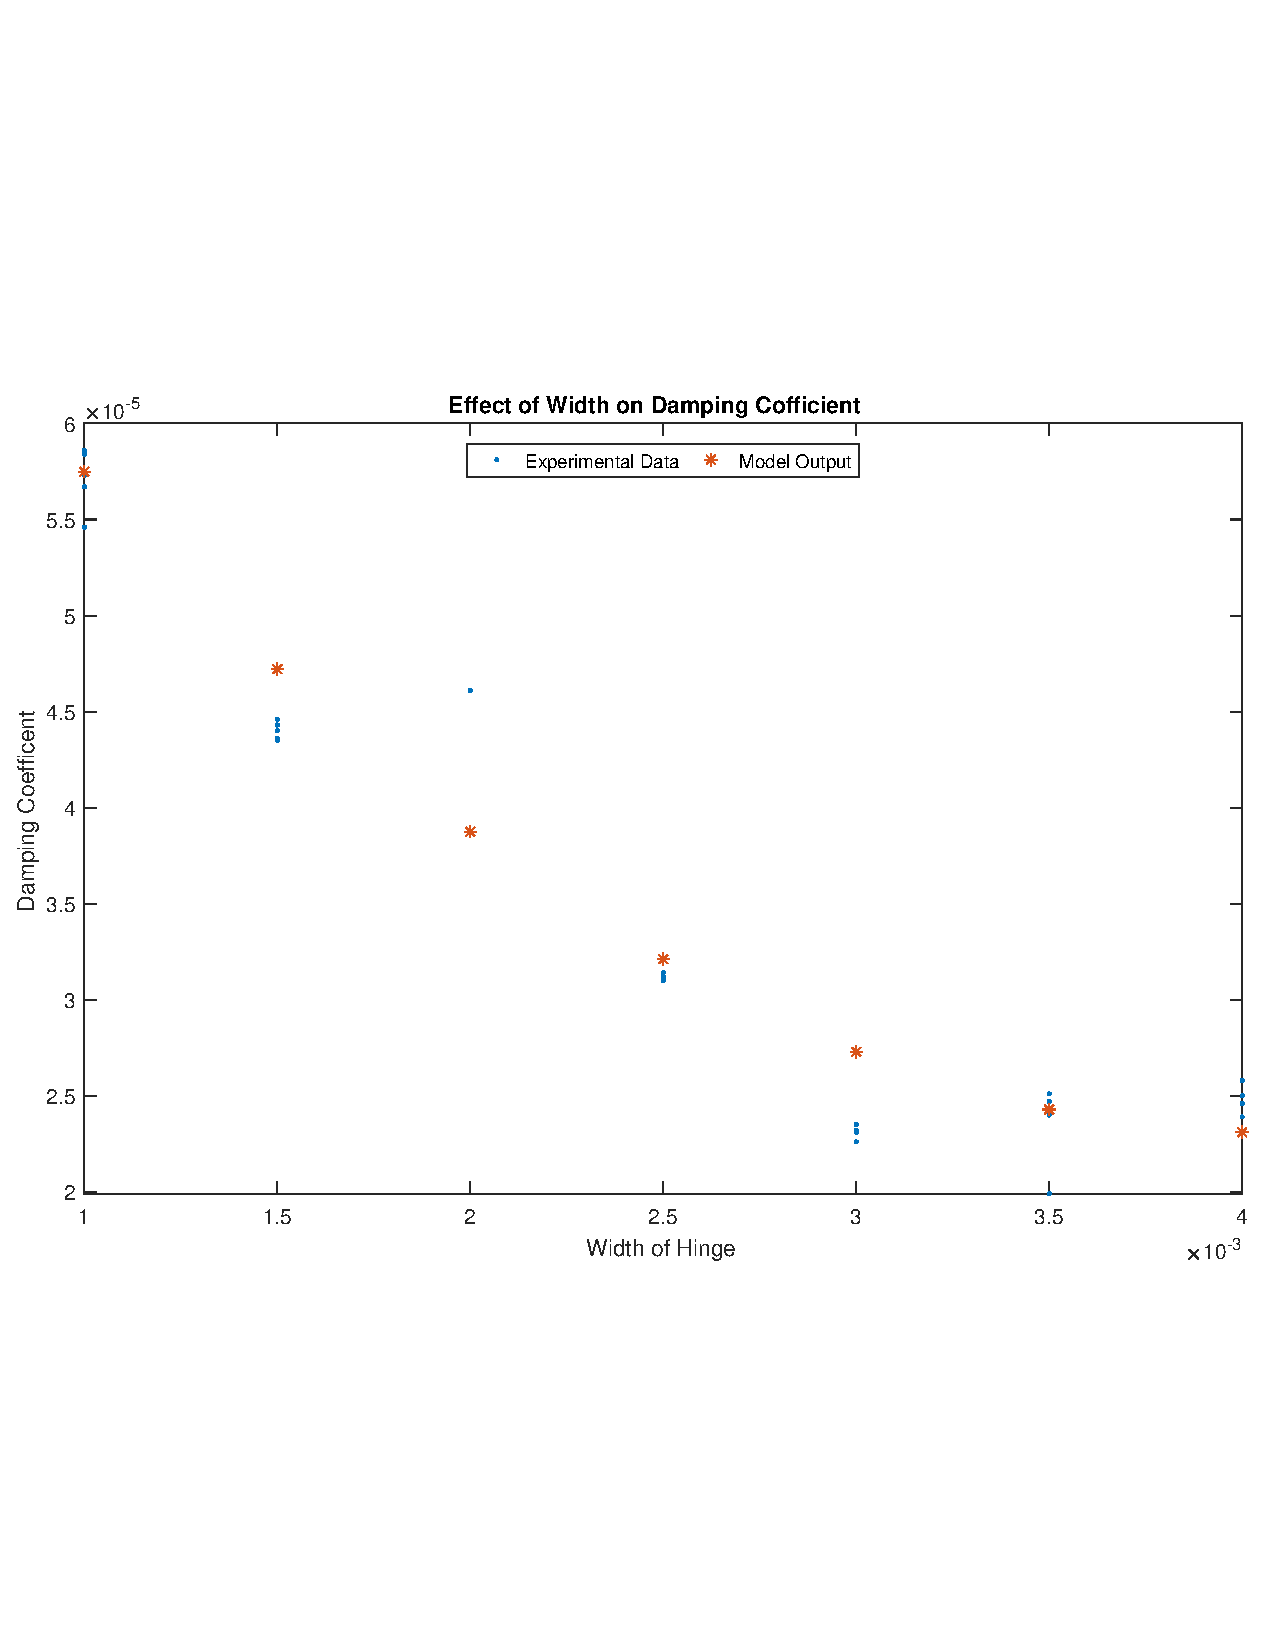
\includegraphics[width=6.5cm]{W_On_C.pdf}
% \end{center}
% \end{block}
% \begin{equation*}
% C = -0.0297 W + 3.6381 W^2 + 8.3506e-05
% \end{equation*}
% \end{frame}

% \begin{frame}{Hinge Characterization}
% \begin{block}{What's effect of change in width on stiffness?}
% \begin{center}
% 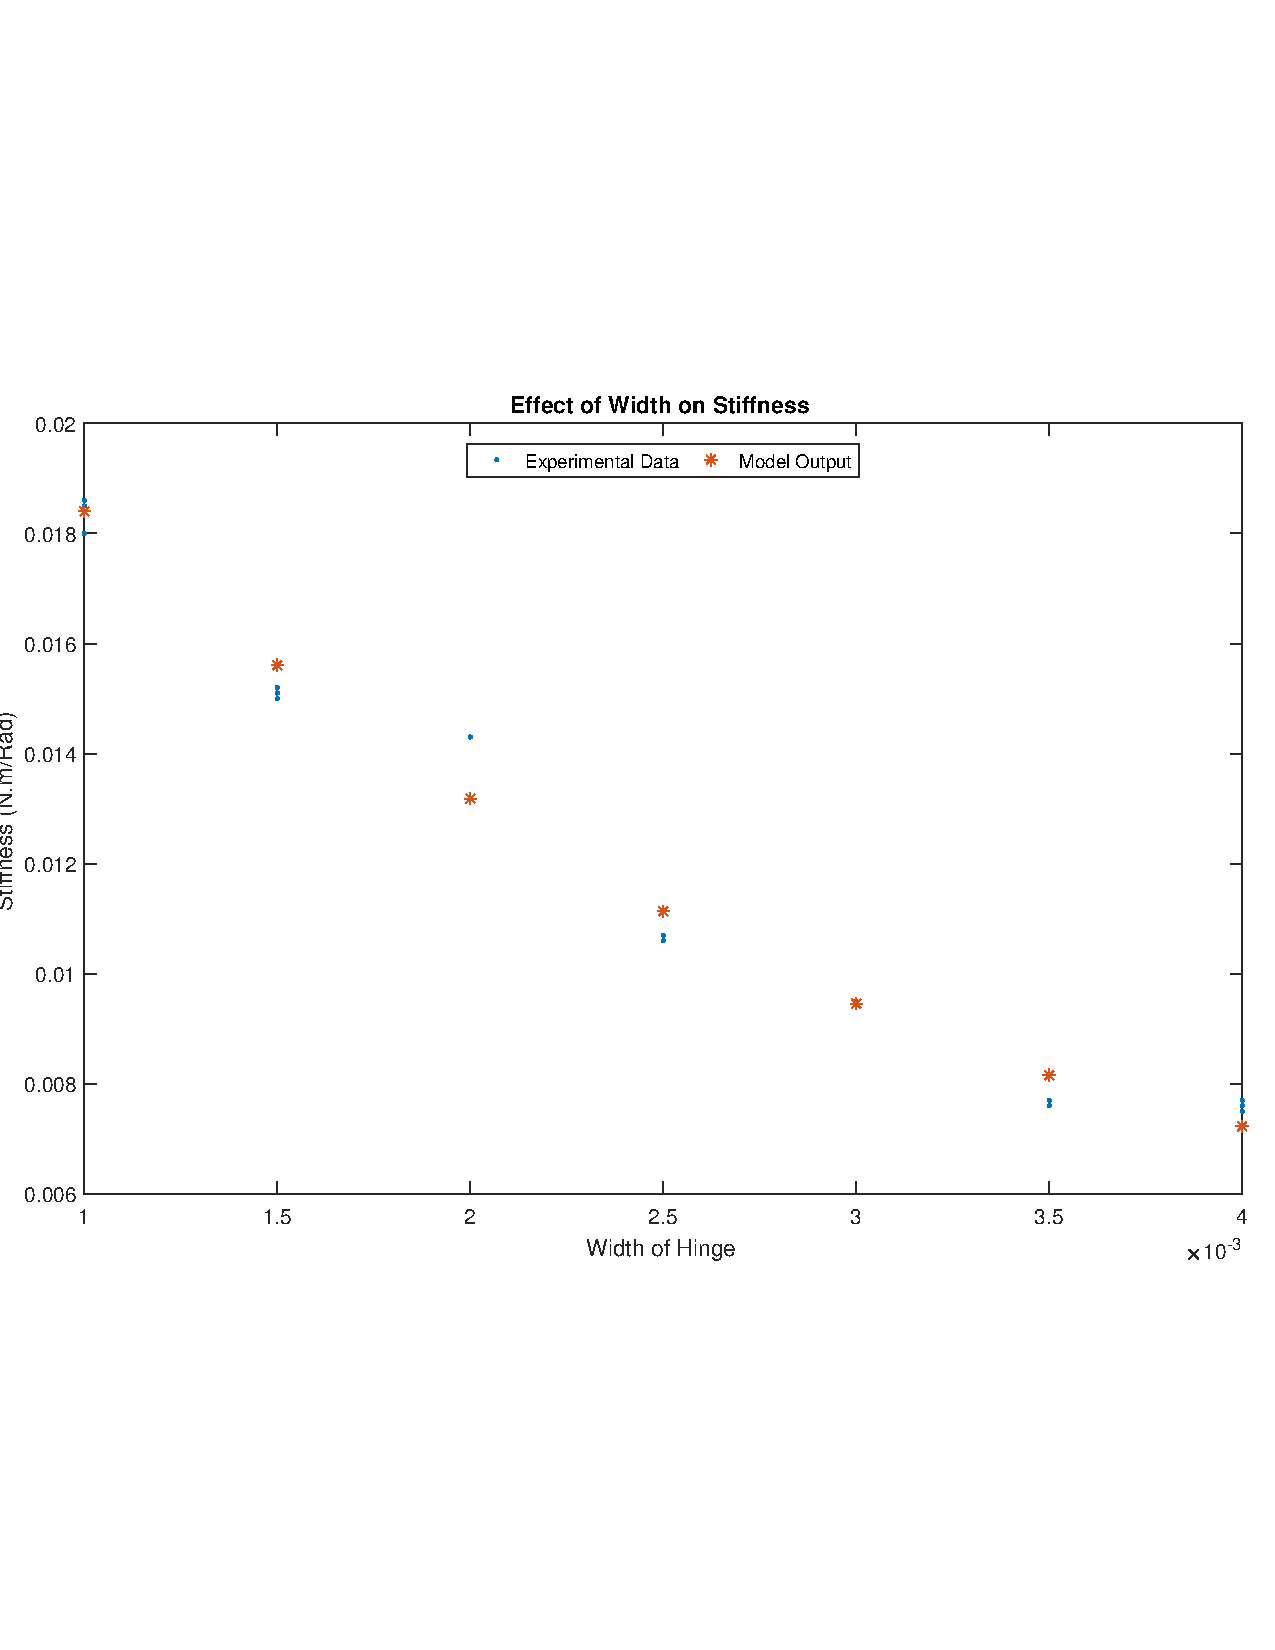
\includegraphics[width=6.5cm]{W_On_K.pdf}
% \end{center}
% \end{block}
% \begin{equation*}
% K = -7.4590 W + 746.6667 W^2 + 0.0251
% \end{equation*}
% \end{frame}

% \subsection{Hinge Length consideration}
% \begin{frame}{Hinge Characterization}
% \begin{block}{What's effect of change in length on damping coefficient?}
% \begin{center}
% 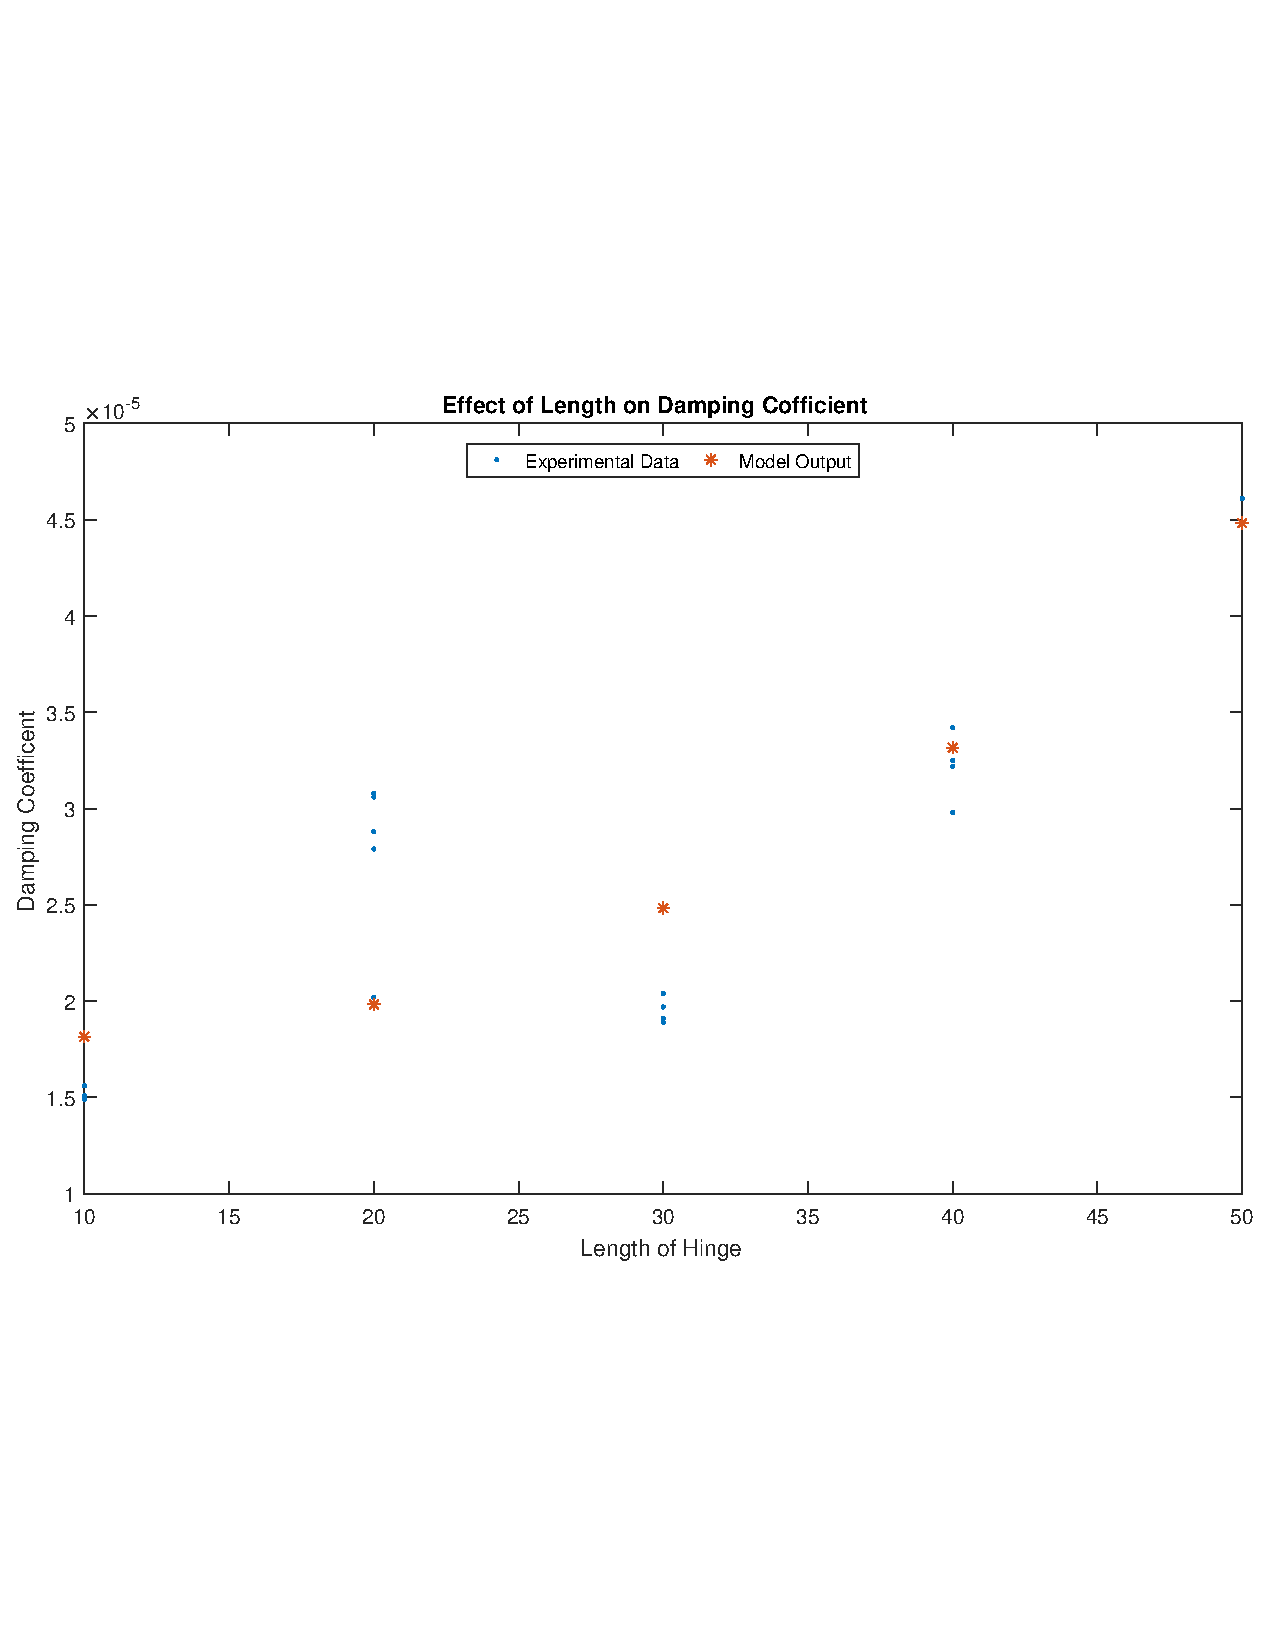
\includegraphics[width=6.5cm]{L_On_C.pdf}
% \end{center}
% \end{block}
% \begin{equation*}
% C = -0.0297 L + 3.6381 L^2 + 8.3506e-05
% \end{equation*}
% \end{frame}

% \begin{frame}{Hinge Characterization}
% \begin{block}{What's effect of change in length on stiffness?}
% \begin{center}
% 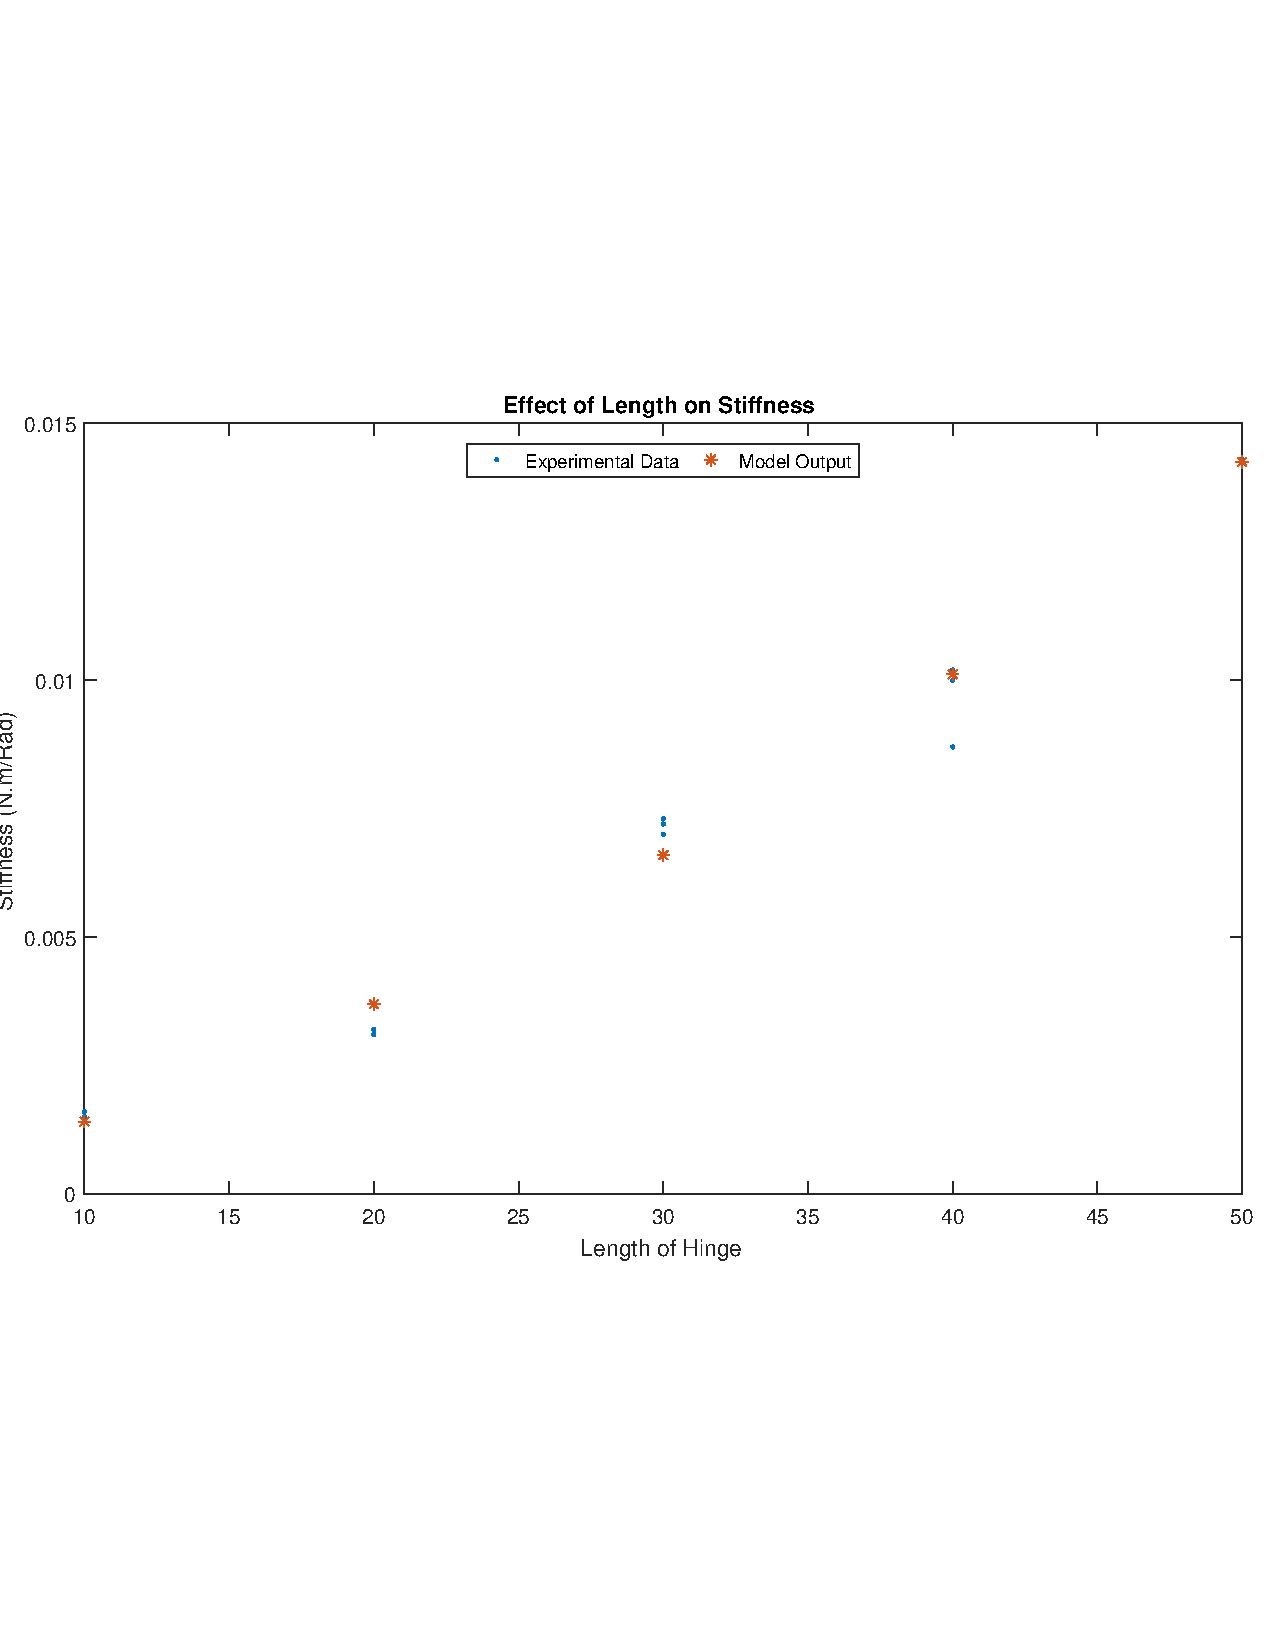
\includegraphics[width=6.5cm]{L_On_K.pdf}
% \end{center}
% \end{block}
% \begin{equation*}
% K = -7.4590 L + 746.6667 L^2 + 0.0251
% \end{equation*}
% \end{frame}


% \subsection{Damping coefficient model}

% \begin{frame}{Hinge Characterization}
% \begin{block}{What's effect of change in length on damping coefficient?}
% \begin{center}
% 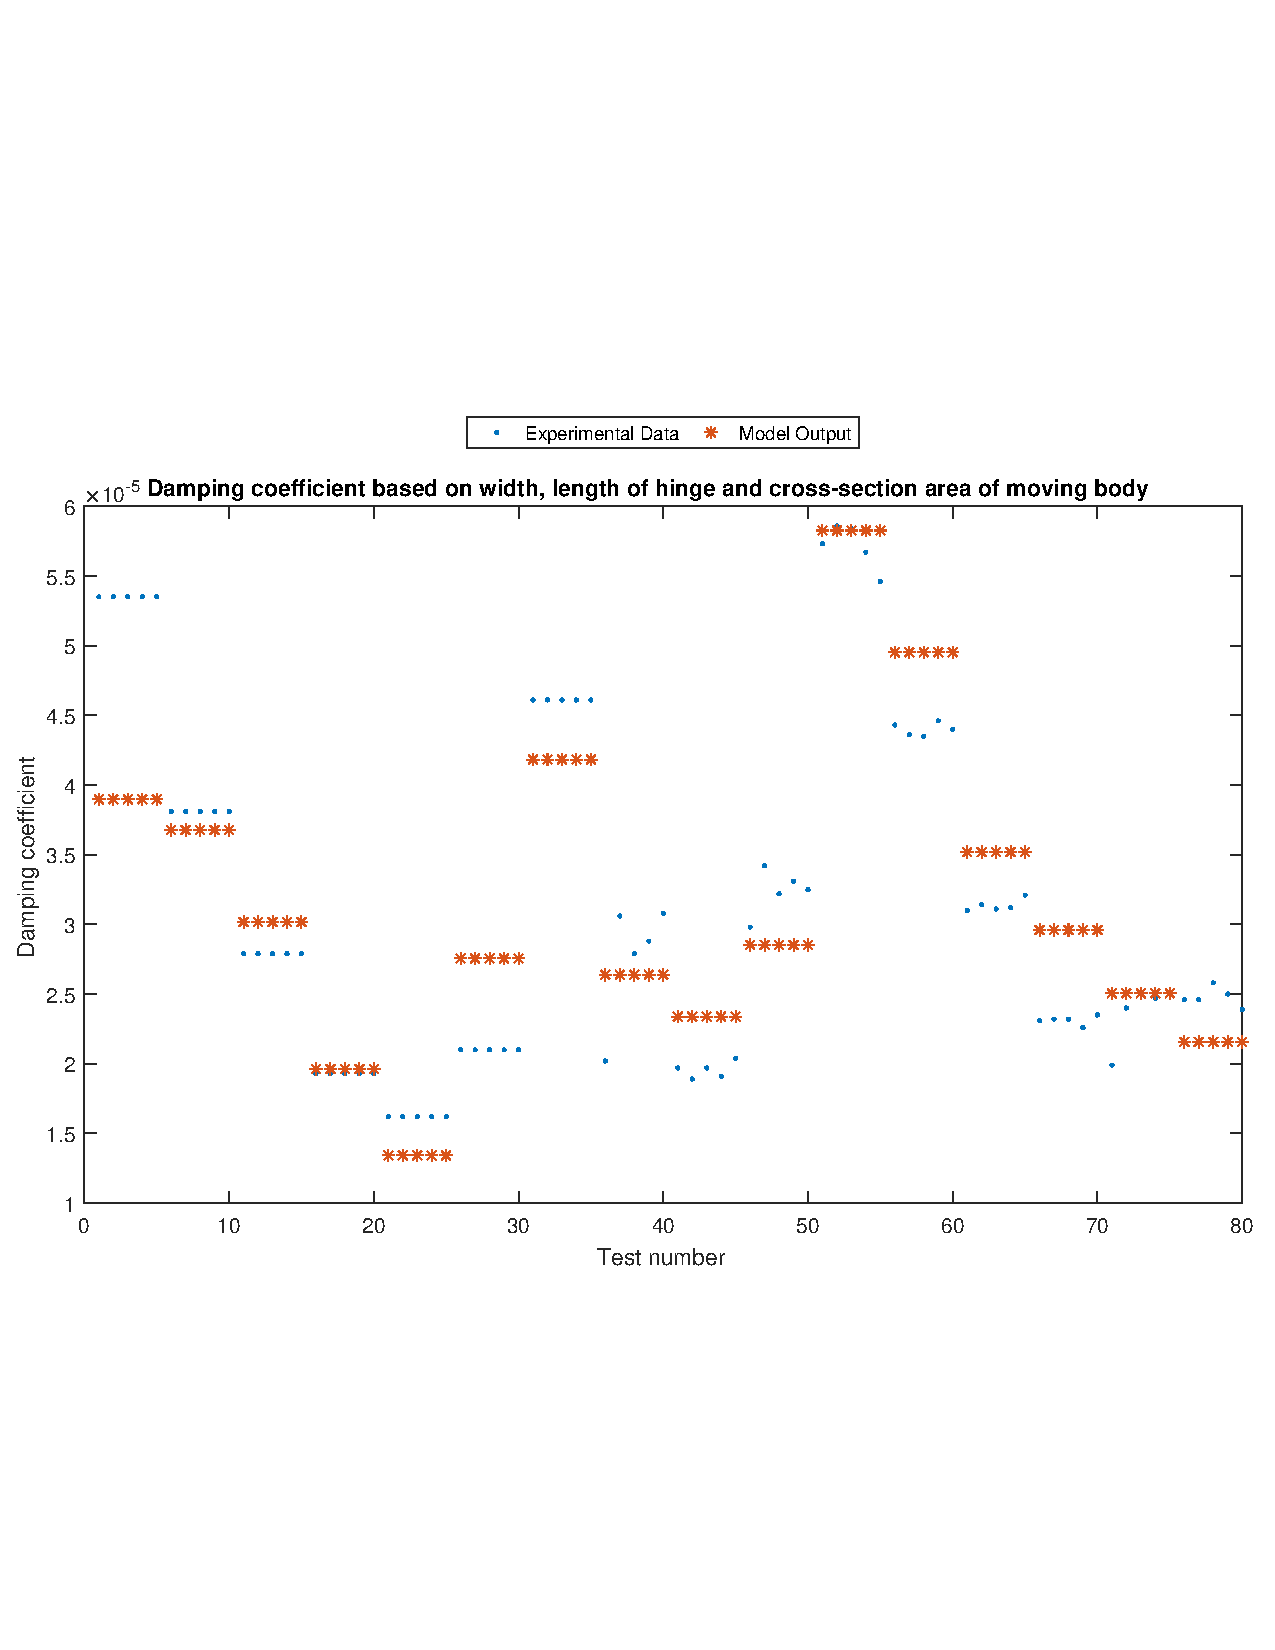
\includegraphics[width=6.5cm]{All_On_C.pdf}
% \end{center}
% \end{block}
% \begin{small}
% \begin{equation*}
% C = 0.0130A - 0.8704 A^2 - 0.0227W + 2.0999W^2 -0.0023L + 0.0407L^2 + 5.0855e-05
% \end{equation*}
% \end{small}
% \end{frame}

% \subsection{Stiffness model}

% \begin{frame}{Hinge Characterization}
% \begin{block}{What's effect of change in length on stiffness?}
% \begin{center}
% 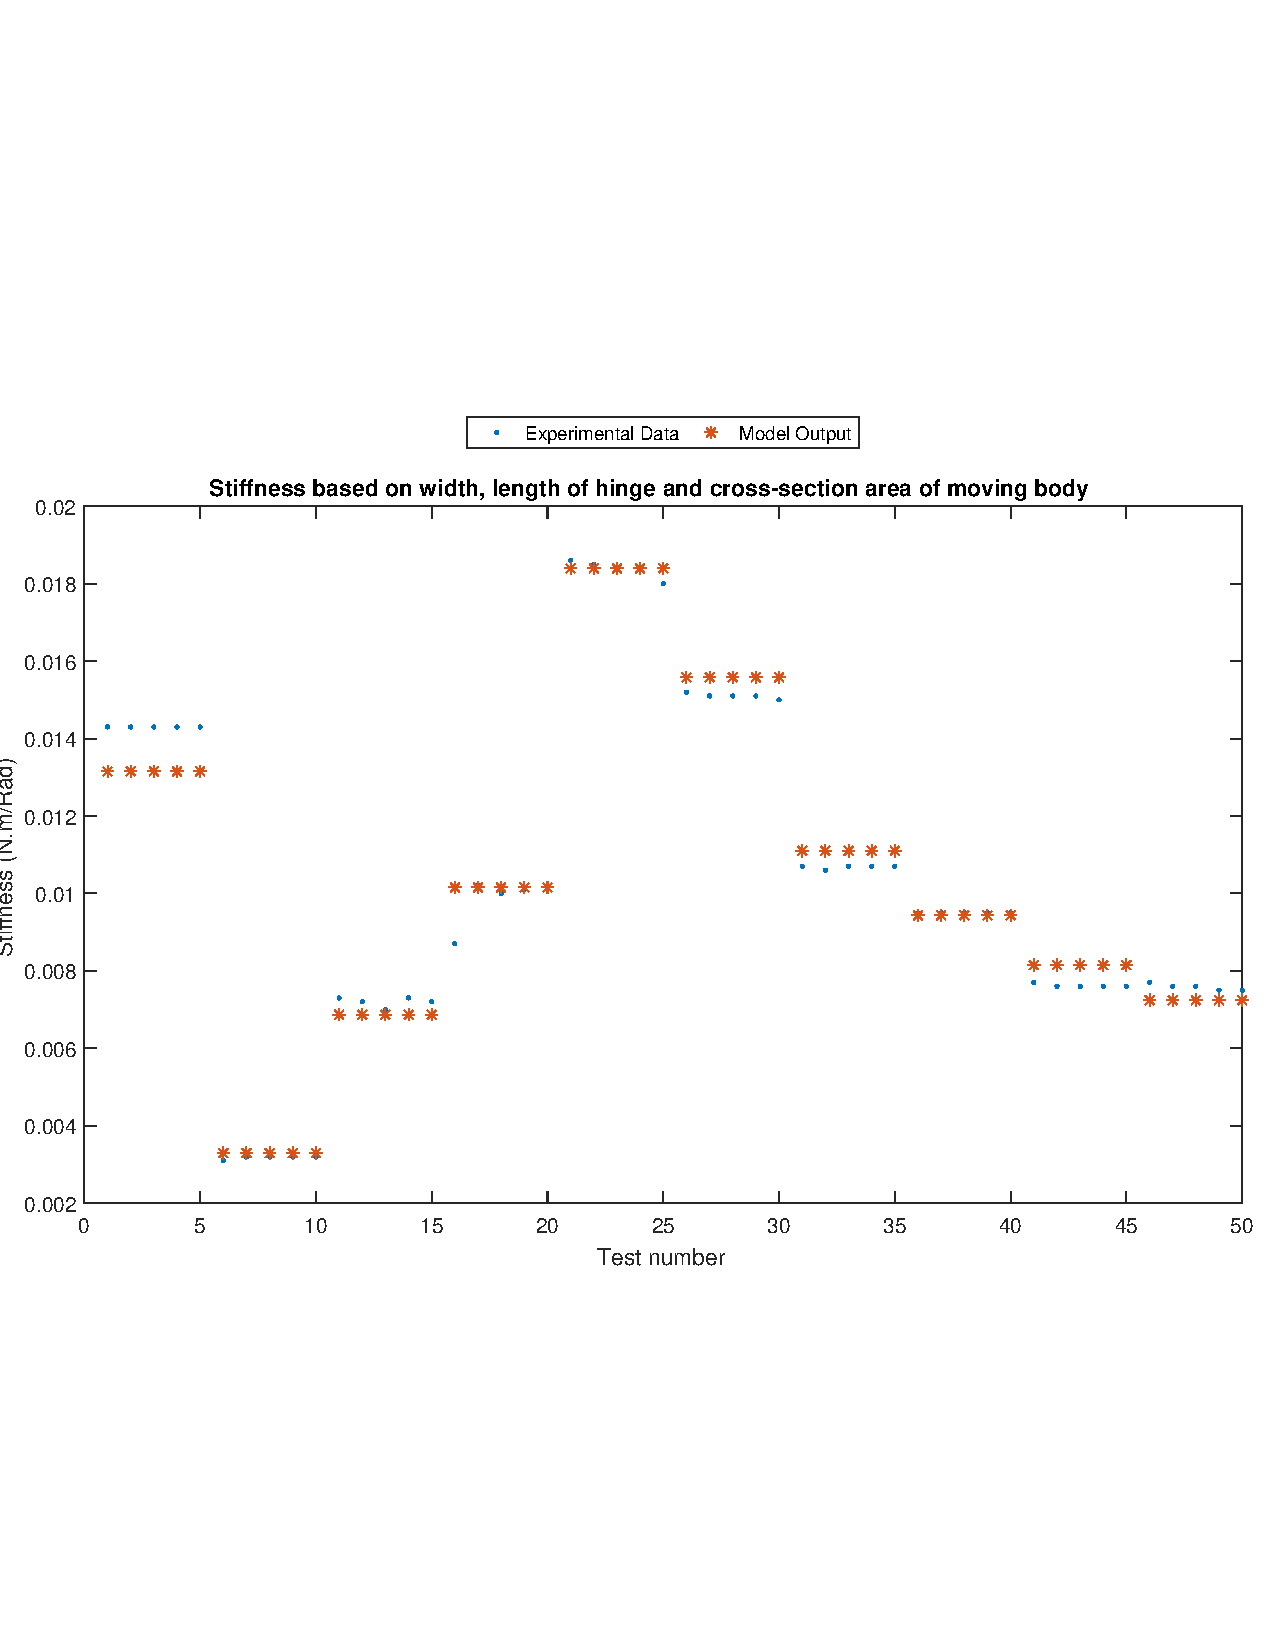
\includegraphics[width=6.5cm]{All_On_K.pdf}
% \end{center}
% \end{block}
% \begin{equation*}
% K = -7.5305 W + 762.5397 W^2 + 0.4298L -1.4444L^2 + 0.0073
% \end{equation*}
% \end{frame}

% \begin{frame}{ONR Project}
% \begin{block}{Molds for Hydro-gel}
% \begin{center}
% 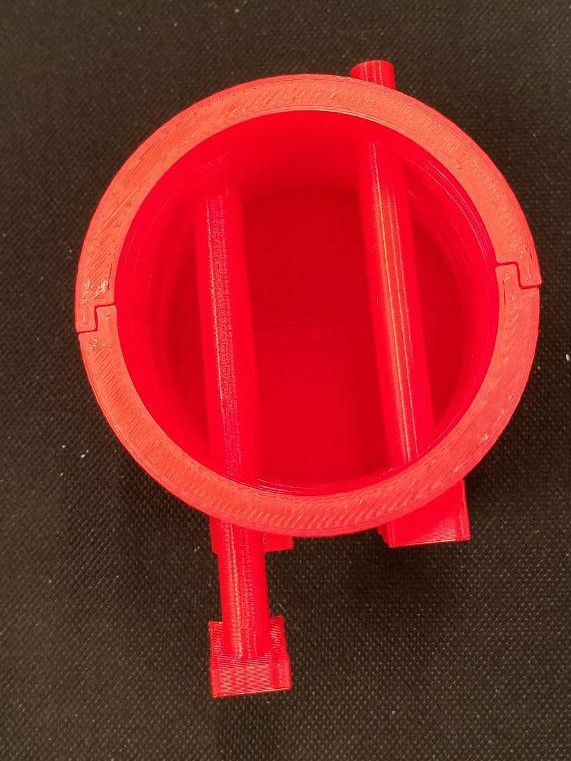
\includegraphics[scale=0.3]{Mold}
% \end{center}
% \end{block}
% \end{frame}

% \section{What's being done?}
% \subsection{Pynamics Paper}
% \begin{frame}{Pynamics paper}
% \begin{block}{Gather data from 3-DOF Spherical mechanism}
% \begin{center}
% 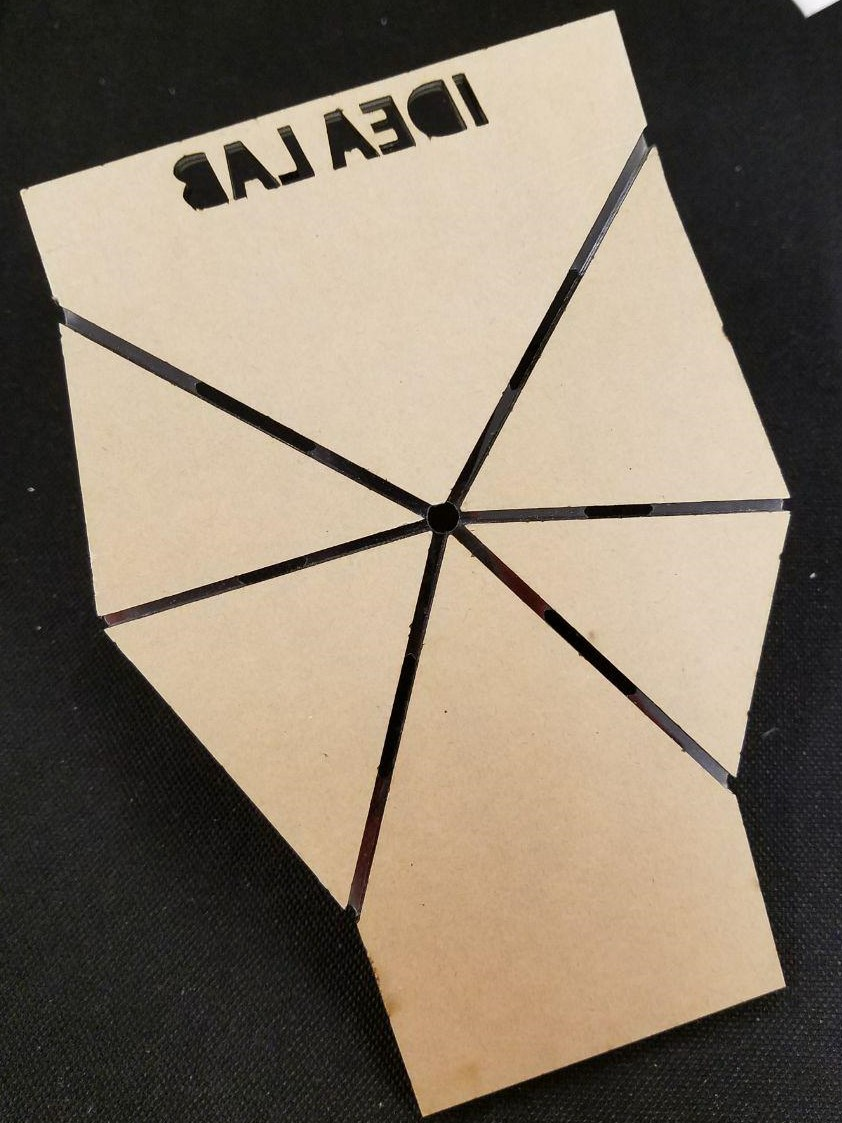
\includegraphics[scale=0.2]{3DOF}
% \end{center}
% \end{block}
% \end{frame}

% \subsection{Summer Robot}
% \begin{frame}{Summer Robot}
% \begin{block}{I'm suggesting}
% \begin{itemize}
% \item Work on a mechanism that a wheel movement to the a flapping movement for a wing...
% \item See if we can attach brushless motors to that...!?
% \end{itemize}
% \end{block}
% \end{frame}

% \begin{frame}
% \frametitle{\emph{Conclusion}}
% \begin{block}{Any Questions...?}
% \begin{center}
% 
\includegraphics[scale=0.7]{questionsk}
% \end{center}
% \end{block}
% \end{frame}



% % ----------------------- Report of 7 July -------------------------
% % ----------------------- Report of 7 July -------------------------
% % ----------------------- Report of 7 July -------------------------


\part{Report of 7 July 2017}
% \frame{\partpage}
% \section{What's Done?}

% \begin{frame}{Review Papers}
% \begin{block}{You will see during the presentation}
% \begin{itemize}
% \item Quaternion Based Inverse Kinematics for Industrial Robot Manipulators with Euler Wrist
% \vspace{1cm}
% %\item \href{run:C:/Users/Mohammad/Google Drive/My read papers/1st Presentation Papers/Bowen.pdf}{Design, Fabrication, and Modeling of an Electro-Magnetic Self-Folding Sheet}
% \item Thermally actuated shape-memory polymers: Experiments, theory,
% and numerical simulations
% \end{itemize}
% \end{block}
% \end{frame}


% % \begin{frame}{Almost finished by the 1st Paper}
% % \begin{block}{What we have done so far:}
% % \begin{itemize}
% % \item Pynamics code is being optimized and ready\\
% % \textcolor{blue} {Thanks to Dan \& Roozbeh 
% % \item Designed and modeled a simple hinge
% % \item I finished the hinge characterization\\
% % Stiffness \& Damping (Material \& Air)
% % \end{itemize}
% % \end{block}
% % \end{frame}


% \begin{frame}{Hinge Characterization}
% \begin{block}{Getting experimental data}
% \begin{itemize}
% \item Get data by using tracking camera
% \item Needs filtering before differentiation\\ 
% Numerical filtering changed the data\\ 
% \hspace{2cm} $\Downarrow$ $\Downarrow$ $\Downarrow$ \\
% $\Rightarrow$ First fit "Fourier Series to data"\\
% $\Rightarrow$ Then apply analytic filtering
% \end{itemize}
% \begin{center}
% 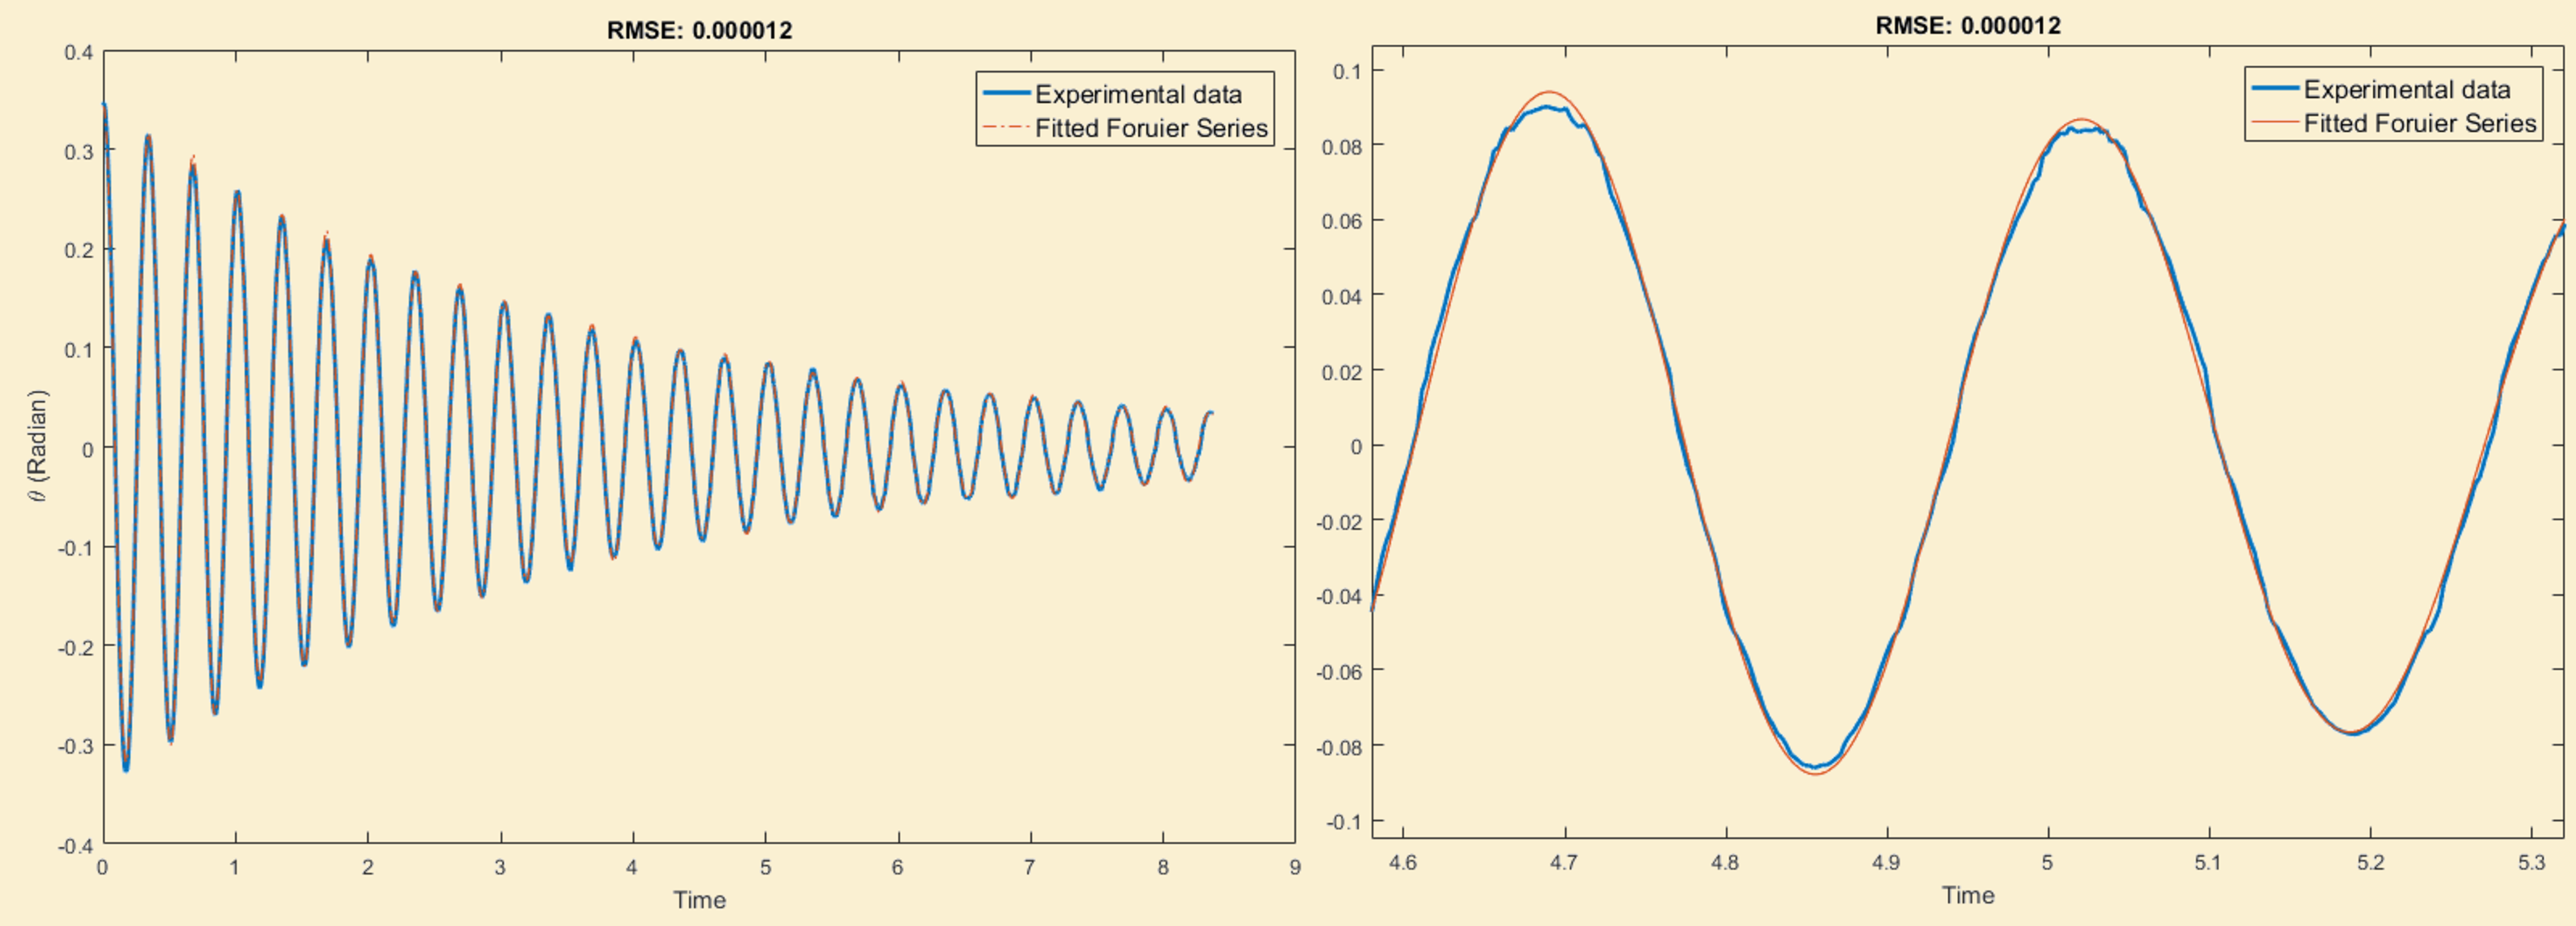
\includegraphics[scale=0.16]{FS_Fit.pdf}
% \end{center}
% \end{block}
% \end{frame}

% \begin{frame}{3DOF Mechanism}
% \begin{block}{Getting experimental data}
% \begin{center}
% 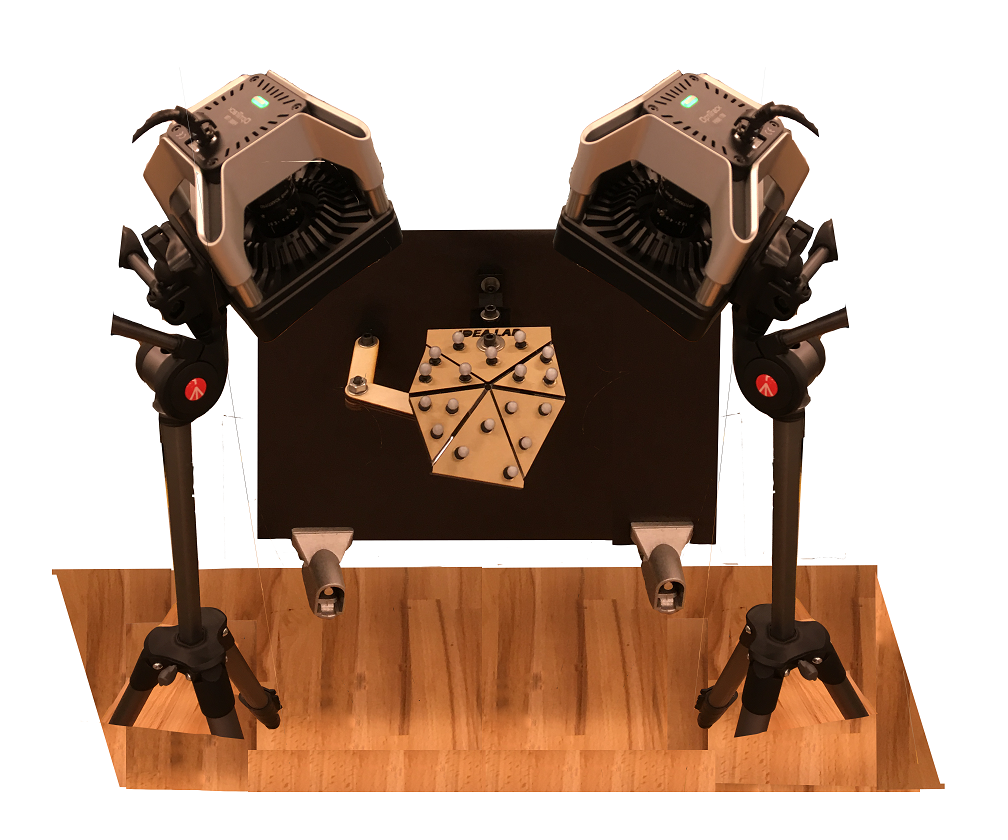
\includegraphics[scale=0.27]{Setup.png}
% \end{center}
% \end{block}
% \end{frame}

% \begin{frame}{3DOF Mechanism}
% \begin{block}{Getting experimental data}
% \begin{itemize}
% \item Get data by using tracking camera
% \item Does not need differentiation\\  
% $\Rightarrow$ Since we are just validating position\\
% $\Rightarrow$ Numerical filtering can be used\\
% \item Data from camera should be processed\\
% \hspace{2cm} $\Downarrow$ $\Downarrow$ $\Downarrow$ \\
% $\Rightarrow$ The Cameras give the position and rotation of the bodies\\
% $\Rightarrow$ We need the joints angle $\Rightarrow$ Sounds like Inverse Kinematic...???
% \end{itemize}
% % \begin{center}
% % 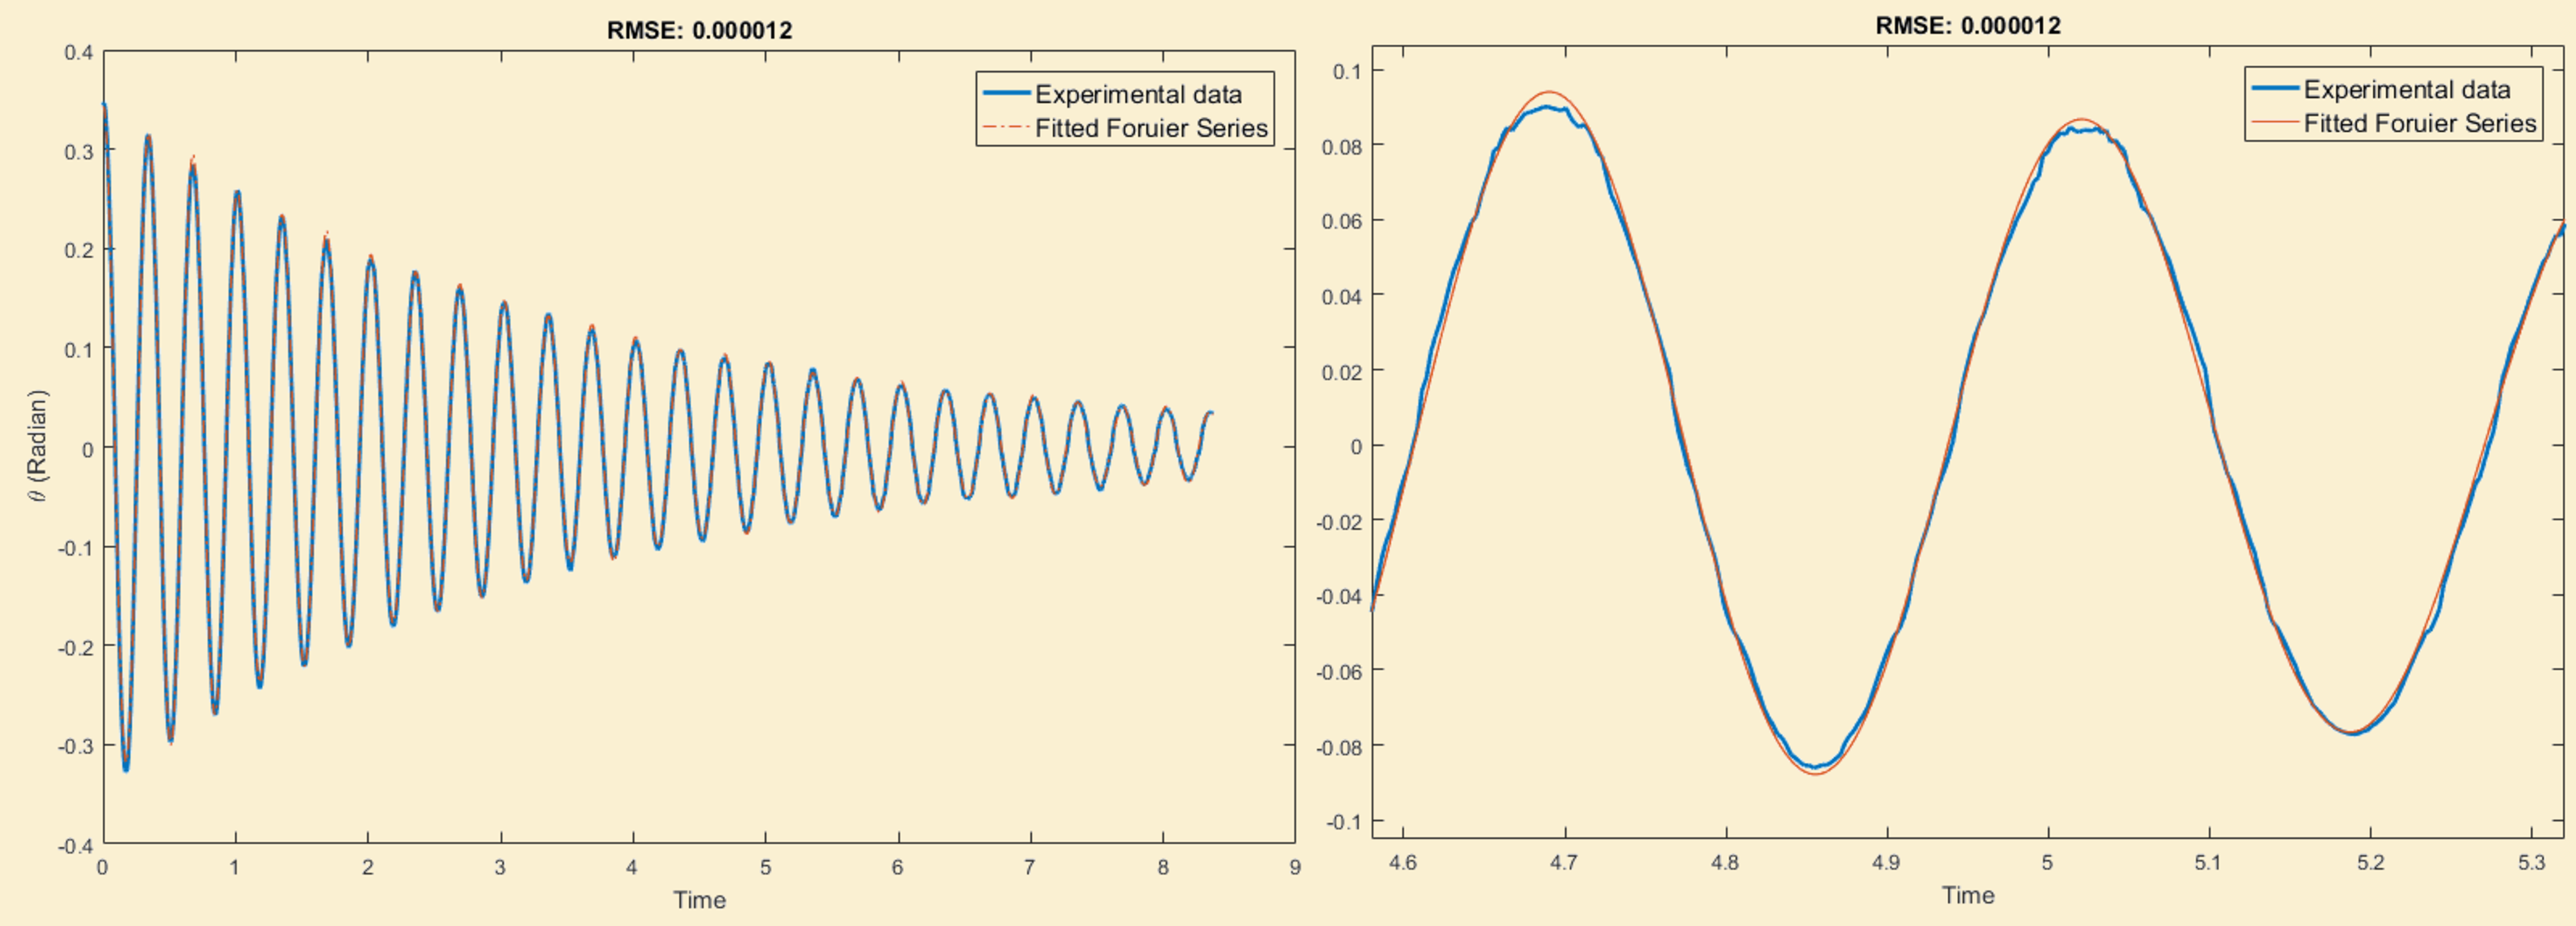
\includegraphics[scale=0.16]{FS_Fit.pdf}
% % \end{center}
% \end{block}
% \end{frame}

% \begin{frame}{3DOF Mechanism}
% \begin{block}{What we have...}
% \begin{itemize}
% \item Data from tracking camera
% \item Position \& orientation of each rigid-bodies\\  
% \end{itemize}
% \end{block}
% \begin{block}{What we want...}
% \begin{itemize}
% \item Joints angle ($\theta_1, \theta_2, \cdots \theta_6$) 
% \item Here comes "\Large $\textbf{Quaternion}$" \normalsize
% \end{itemize}
% \end{block}
% \end{frame}

% \begin{frame}{3DOF Mechanism}
% \begin{block}{What's Quaternion...???}
% \begin{itemize}
% \item It's a method to show the orientation in 3D
% \item Involves 4 parameters
% \item one Scaler ($s = q_w$) \quad \& \quad one vector ($v = [q_x q_y q_z]$)
% \item Interesting connection with Complex numbers...!!!!
% \end{itemize}
% \end{block}
% \begin{block}{What's the idea behind it...?}
% \begin{center}
% 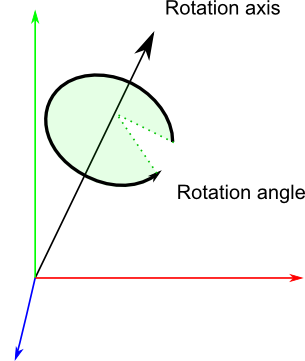
\includegraphics[scale=0.22]{quaternion.png}
% \end{center}
% \end{block}
% \end{frame}

% \begin{frame}{Review Papers}
% \begin{block}{Using Quaternion in IKP}
% \begin{itemize}
% \item \href{run:C:/Users/Mohammad/Google Drive/My read papers/2nd Presentation Papers/Quaternion Based Inverse Kinematics.pdf}{Quaternion Based Inverse Kinematics for Industrial Robot Manipulators with Euler Wrist}
% \end{itemize}
% \end{block}
% \end{frame}

% \begin{frame}{3DOF Mechanism}
% \begin{block}{We got the angles out}
% \begin{center}
% 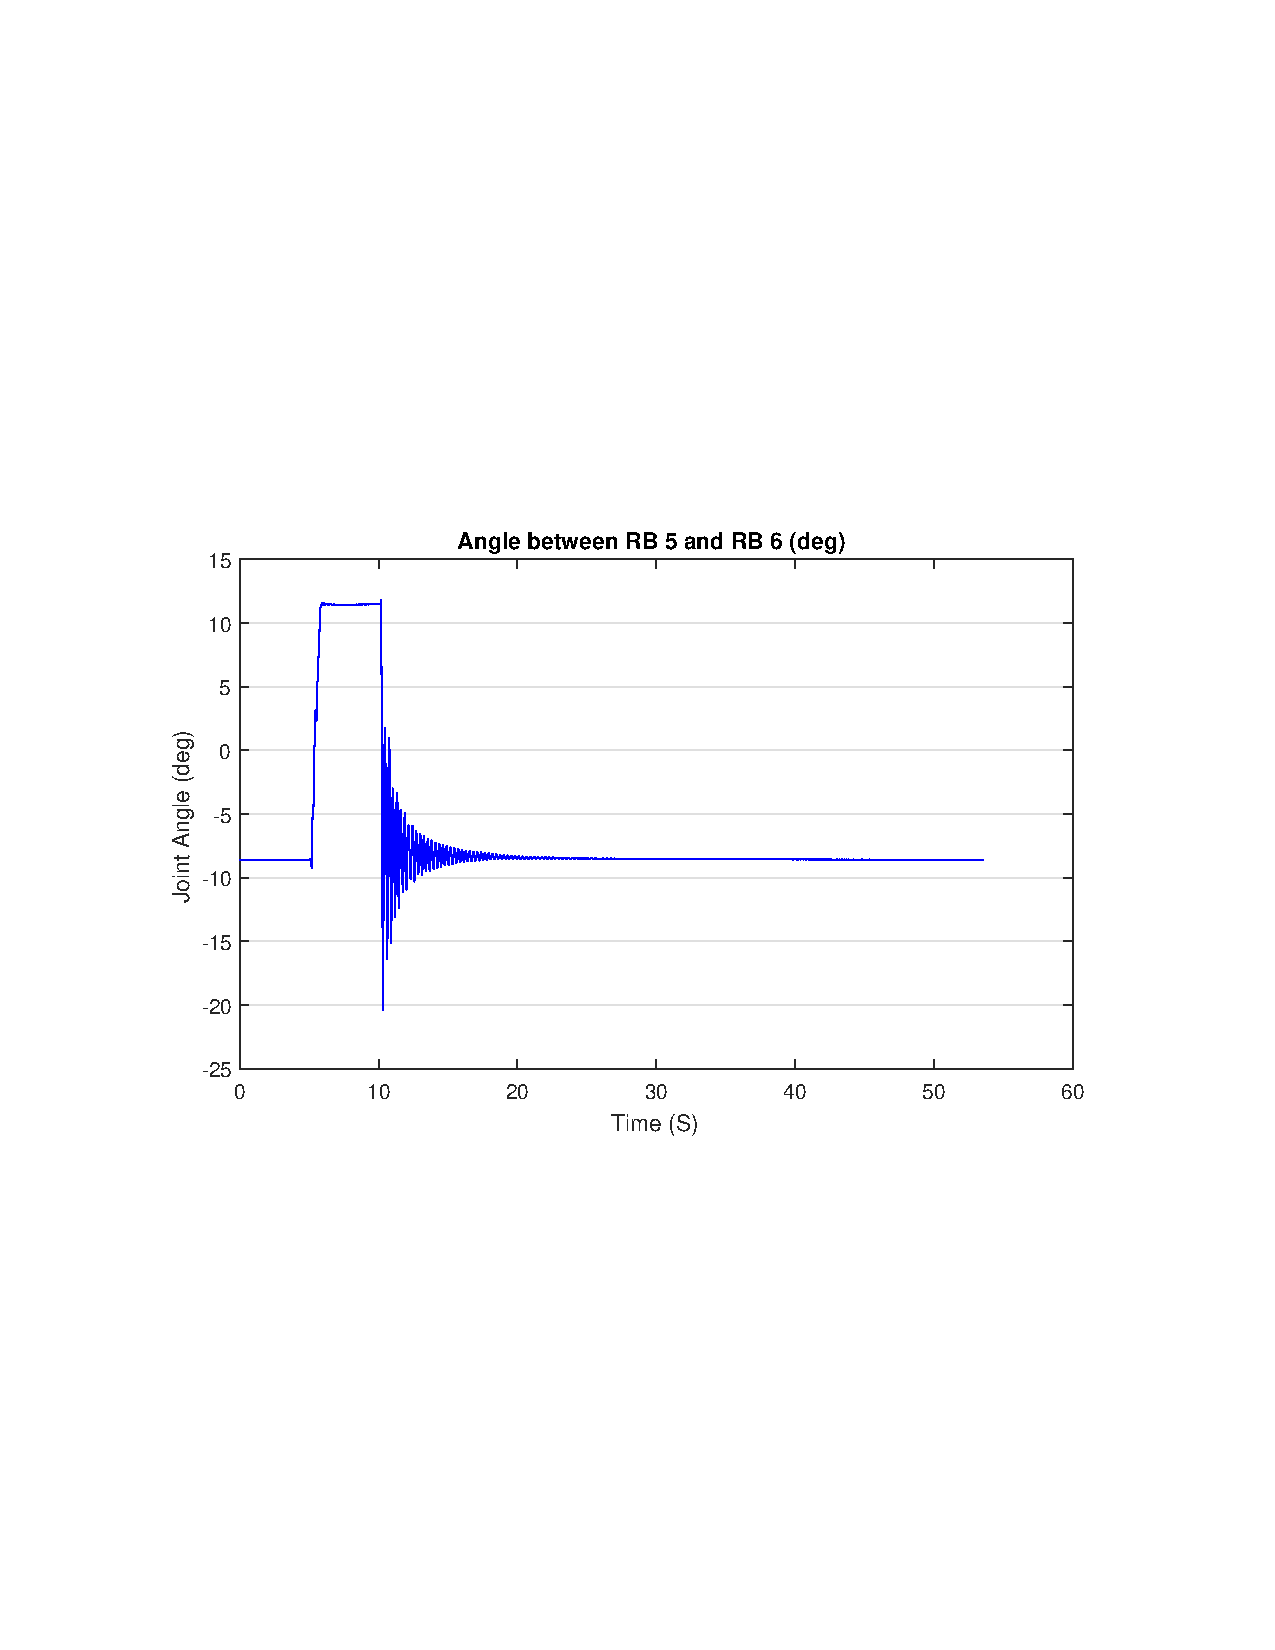
\includegraphics[scale=0.56]{R56.pdf}
% \end{center}
% \end{block}
% \end{frame}

% \begin{frame}{Hydrogel Material property test}
% \begin{block}{What we are seeking...???}
% \begin{itemize}
% \item We seek the stress-strain relation
% \item Compression VS Load 
% \item What the deformation looks like?
% \item Any interesting behavior?
% \end{itemize}
% \end{block}
% \end{frame}

% \begin{frame}{Hydrogel Material property test}
% \begin{block}{I've prepared a report!}
% \begin{itemize}
% \item \href{run:C:/Users/Mohammad/Google Drive/idealab/ONR Project/Material Testing/Report-material-test.pdf}{Report File}
% \item \href{run:C:/Users/Mohammad/Google Drive/idealab/ONR Project/Material Testing/LT.gif}{Low Temperature Hydrogel}
% \item \href{run:C:/Users/Mohammad/Google Drive/idealab/ONR Project/Material Testing/HT.gif}{High Temperature Hydrogel}

% \end{itemize}
% \end{block}
% \end{frame}

% \begin{frame}{Review Papers}
% \begin{block}{Thermally actuated Material Characterization}
% \begin{itemize}
% \item \href{run:C:/Users/Mohammad/Google Drive/My read papers/2nd Presentation Papers/Thermally actuated SMP.pdf}{Thermally actuated shape-memory polymers: Experiments, theory,
% and numerical simulations}
% \end{itemize}
% \end{block}
% \end{frame}

% \begin{frame}{Robot Arm Purchase}
% \begin{block}{Robots we searched through}
% \begin{columns}
% \column{3.5cm}	
% \begin{itemize}
% \alt<1>{\color{blue} \item Universal Robotics}{\color{gray} \item Universal Robotics}
% \alt<2>{\color{blue} \item KUKA}{\color{gray} \item KUKA}
% \alt<3>{\color{blue} \item Kinova}{\color{gray} \item Kinova}
% \alt<4>{\color{blue} \item Denso}{\color{gray} \item Denso}
% \alt<5>{\color{blue} \item Omron - Adept}{\color{gray} \item Omron - Adept}
% \alt<6>{\color{blue} \item Mecademic}{\color{gray} \item Mecademic}
% \end{itemize}
% \column{7cm}
% \only<1>{\begin{figure}[h]\resizebox{!}{3.5cm}{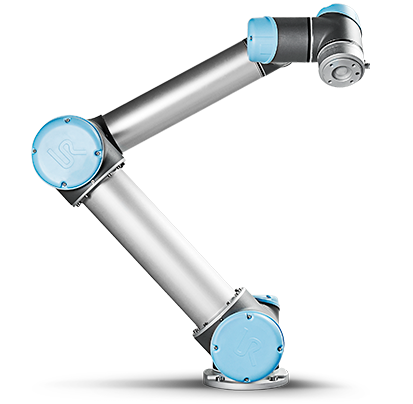
\includegraphics{ur5.png}} \end{figure}
% \begin{center}
% \Large UR5\\ 25,000\$ \normalsize
% \end{center}}
% \only<2>{\begin{figure}[h]\resizebox{!}{3.5cm}{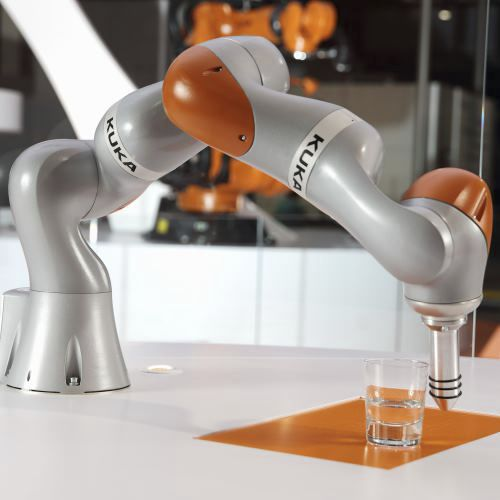
\includegraphics{LBR}} \end{figure}
% \begin{center}
% \Large LBR iiwa 7 R800\\ 65,000\$ \normalsize
% \end{center}}
% \only<3>{\begin{figure}[h]\resizebox{!}{4cm}
% {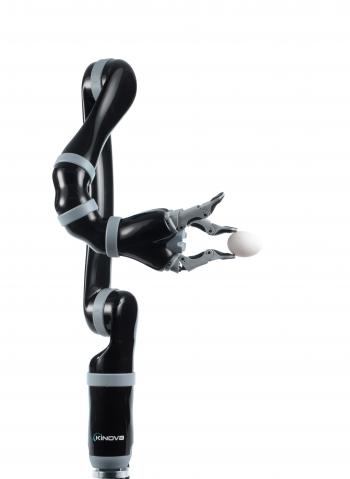
\includegraphics{jaco.jpg}} \end{figure}
% \begin{center}
% \Large Jaco2-6DOF Spherical\\ 30,000\$ \normalsize
% \end{center}}
% \only<4>{\begin{figure}[h]\resizebox{!}{3.5cm}
% {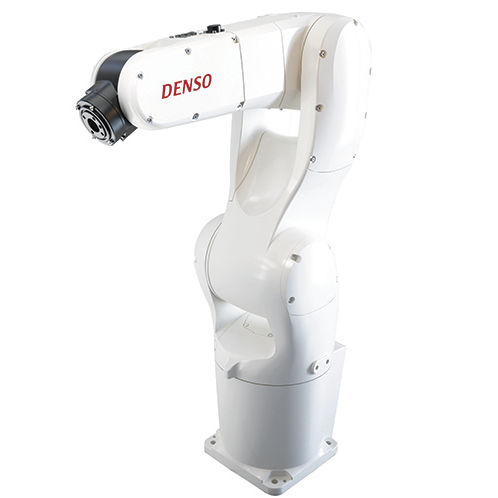
\includegraphics{VS60.jpg}} \end{figure}
% \begin{center}
% \Large VS-060\\ 30,000\$ \normalsize
% \end{center}}
% \only<5>{\begin{figure}[h]\resizebox{!}{3.5cm}
% {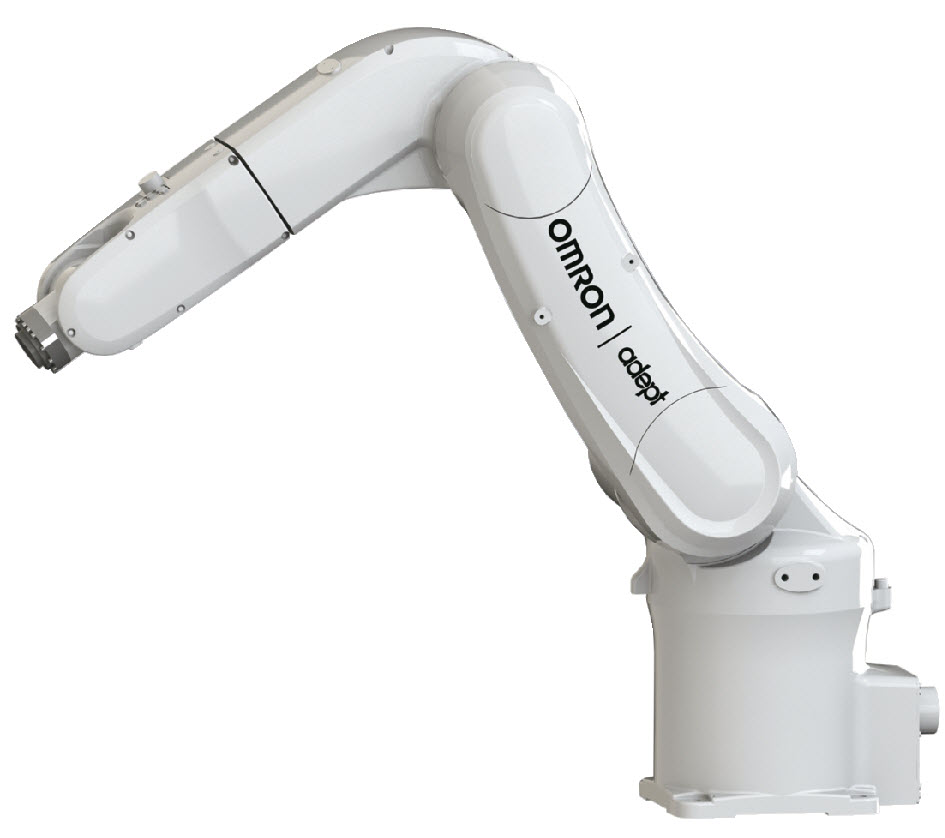
\includegraphics{Viper.jpg}} \end{figure}
% \begin{center}
% \Large Viper 650\\ 28,000\$ \normalsize
% \end{center}}
% \only<6>{\begin{figure}[h]\resizebox{!}{3.5cm}
% {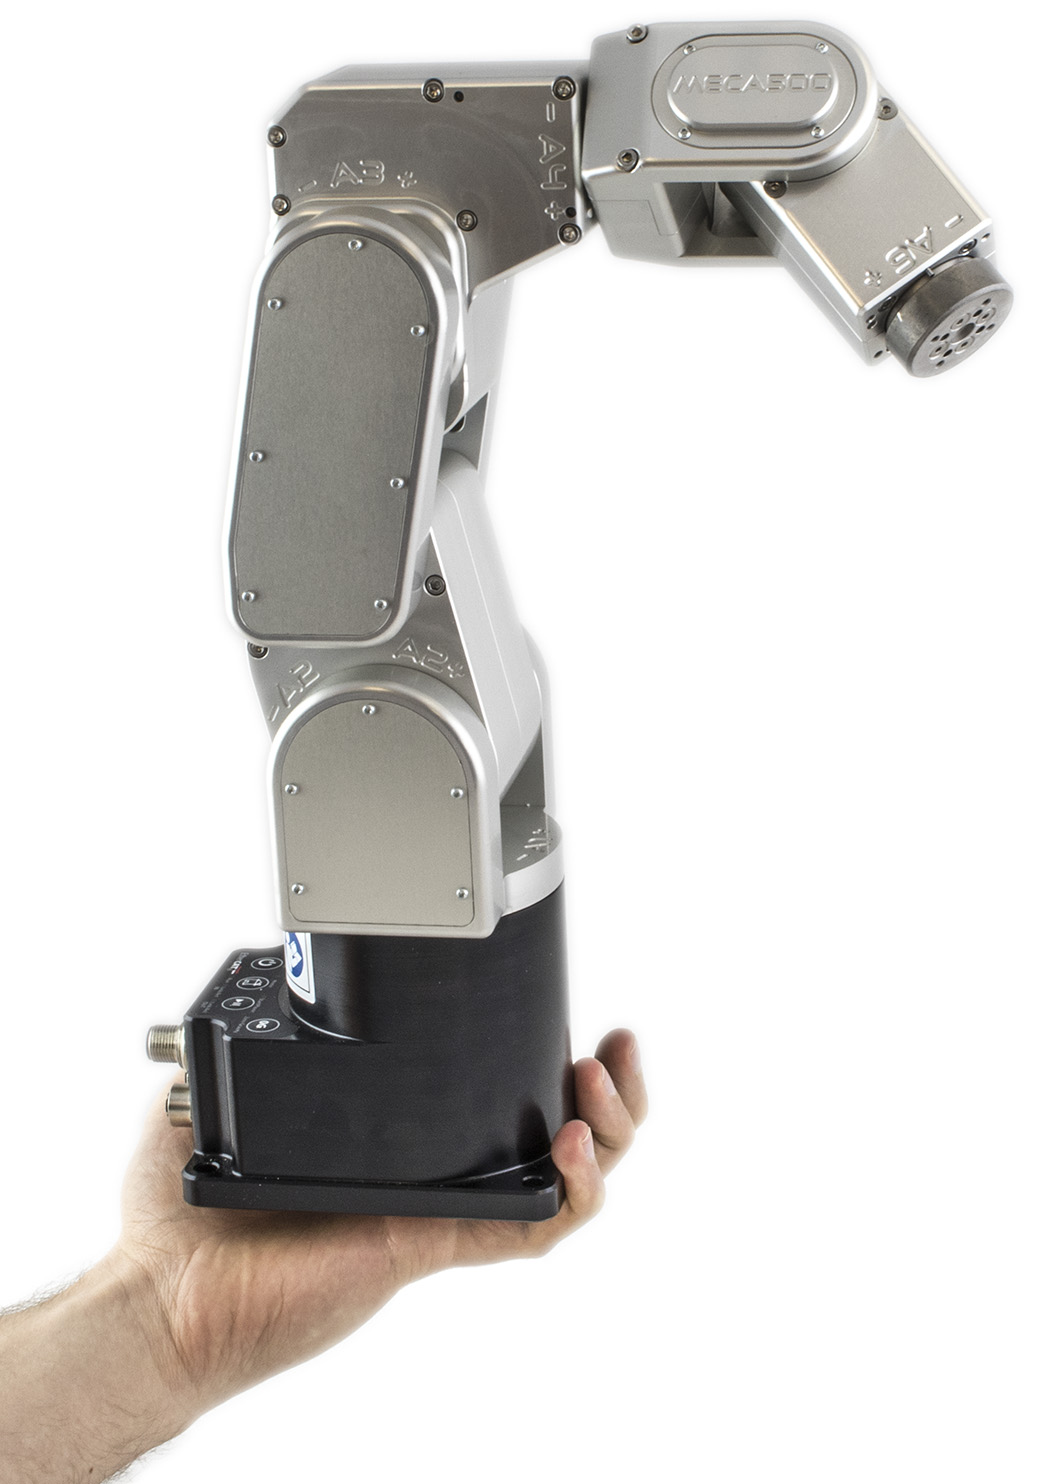
\includegraphics{Meca500.jpg}} \end{figure}
% \begin{center}
% \Large Meca500\\ 15,000\$ \normalsize
% \end{center}}
% \end{columns}
% \end{block}
% \end{frame}

% \begin{frame}{Robot Arm Purchase}
% \begin{block}{Ranked First}
% \begin{center}
% 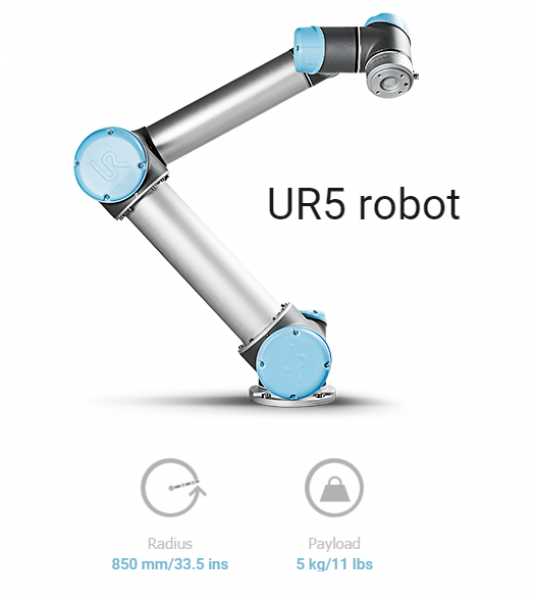
\includegraphics[scale=0.3]{UR5_sel.png}
% % \Large The Ugly cute one :) \normalsize
% \end{center}
% \end{block}
% \end{frame}

% \begin{frame}{Robot Arm Purchase}
% \begin{block}{Force Sensors searched through}
% \begin{columns}
% \column{2.5cm}	
% \begin{itemize}
% \alt<1>{\color{blue} \item ATI}{\color{gray} \item ATI}
% \alt<2>{\color{blue} \item Robotiq}{\color{gray} \item Robotiq}
% \alt<3>{\color{blue} \item OptoForce}{\color{gray} \item OptoForce}
% \end{itemize}
% \column{9cm}
% \only<1>{\begin{figure}[h]\resizebox{!}{4cm}{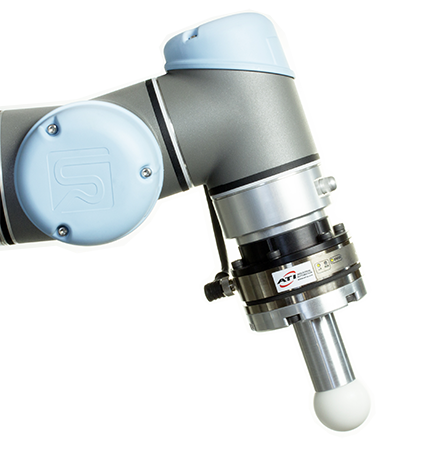
\includegraphics{Axia80.png}} \end{figure}
% \begin{center}
% \Large ATI AXIA80\\ 3650\$ \normalsize
% \end{center}}
% \only<2>{\begin{figure}[h]\resizebox{!}{4.0cm}{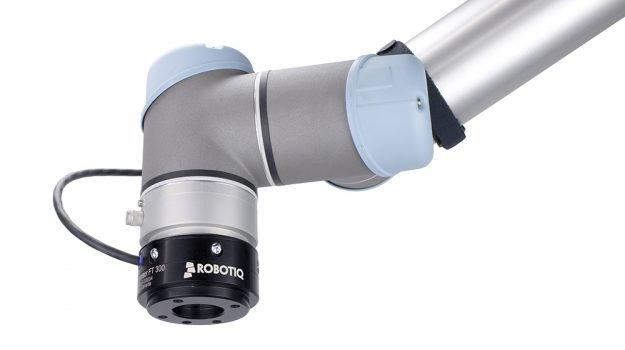
\includegraphics{FT300}} \end{figure}
% \begin{center}
% \Large FT300\\ 4400\$ \normalsize
% \end{center}}
% \only<3>{\begin{figure}[h]\resizebox{!}{4.0cm}
% {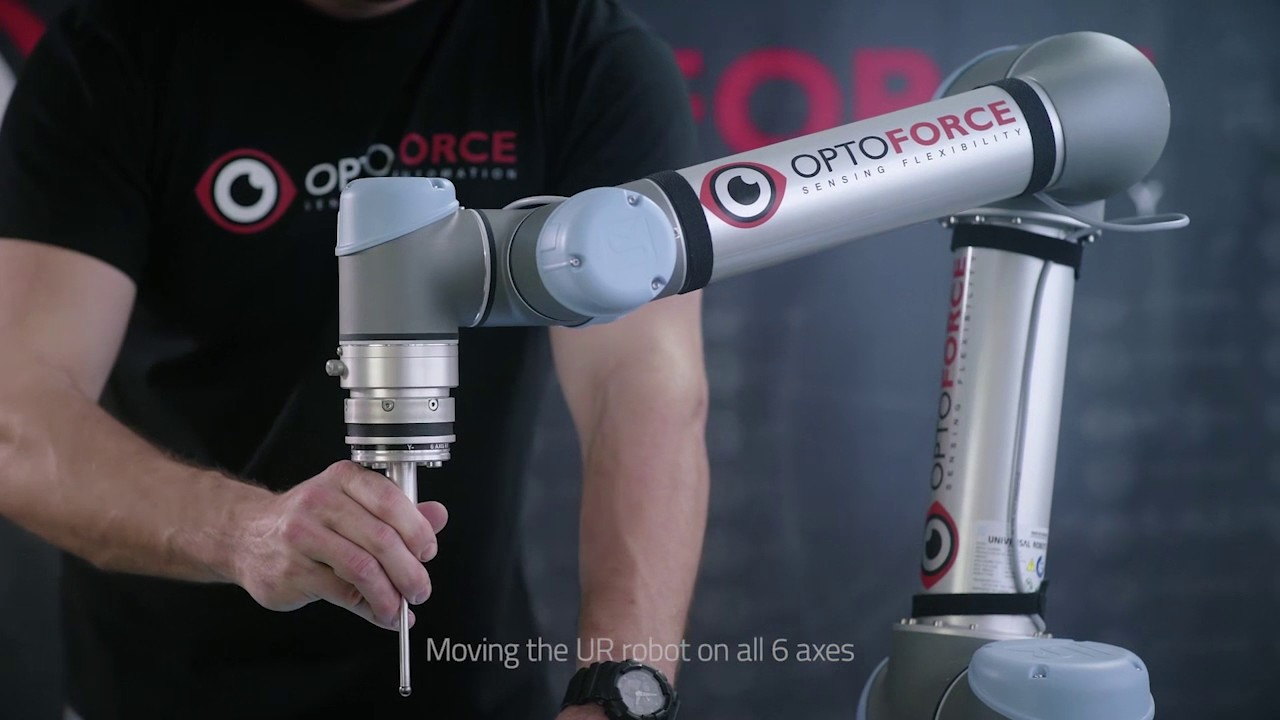
\includegraphics{opto.jpg}} \end{figure}
% \begin{center}
% \Large H E X-7 0 -X E- 200N\\ 4,420\$ \normalsize
% \end{center}}
% \end{columns}
% \end{block}
% \end{frame}

% \begin{frame}{Wing Flapping}
% \begin{block}{The first Prototype}
% \begin{center}
% 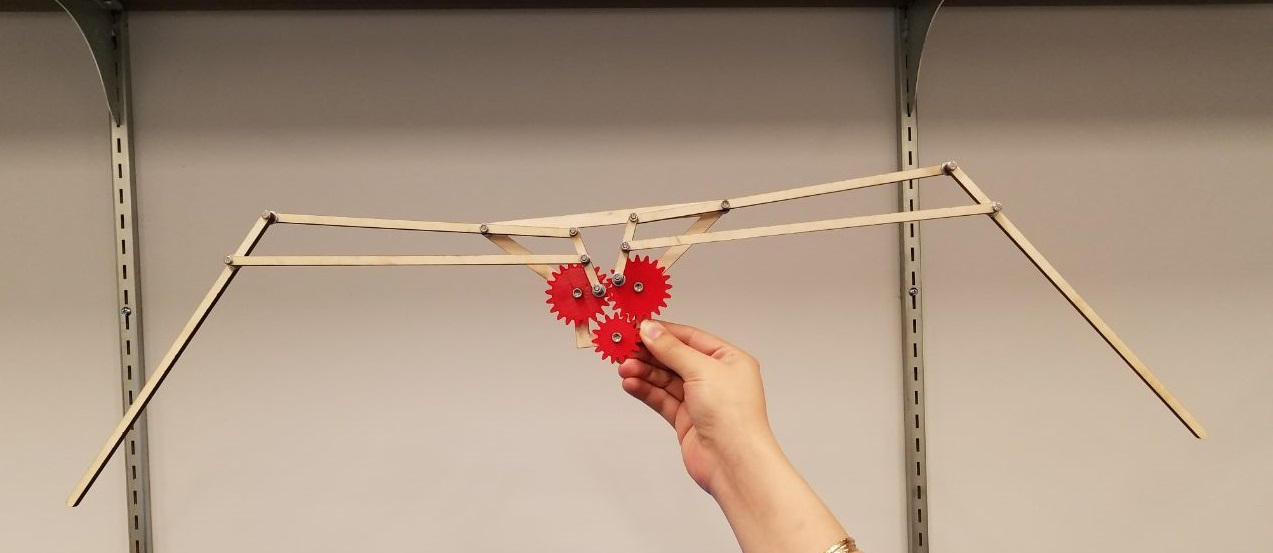
\includegraphics[scale=0.36]{Wing}
% \end{center}
% \end{block}
% \end{frame}

% \begin{frame}{Wing Flapping}
% \begin{block}{Wrote down FKP}
% \begin{center}
% 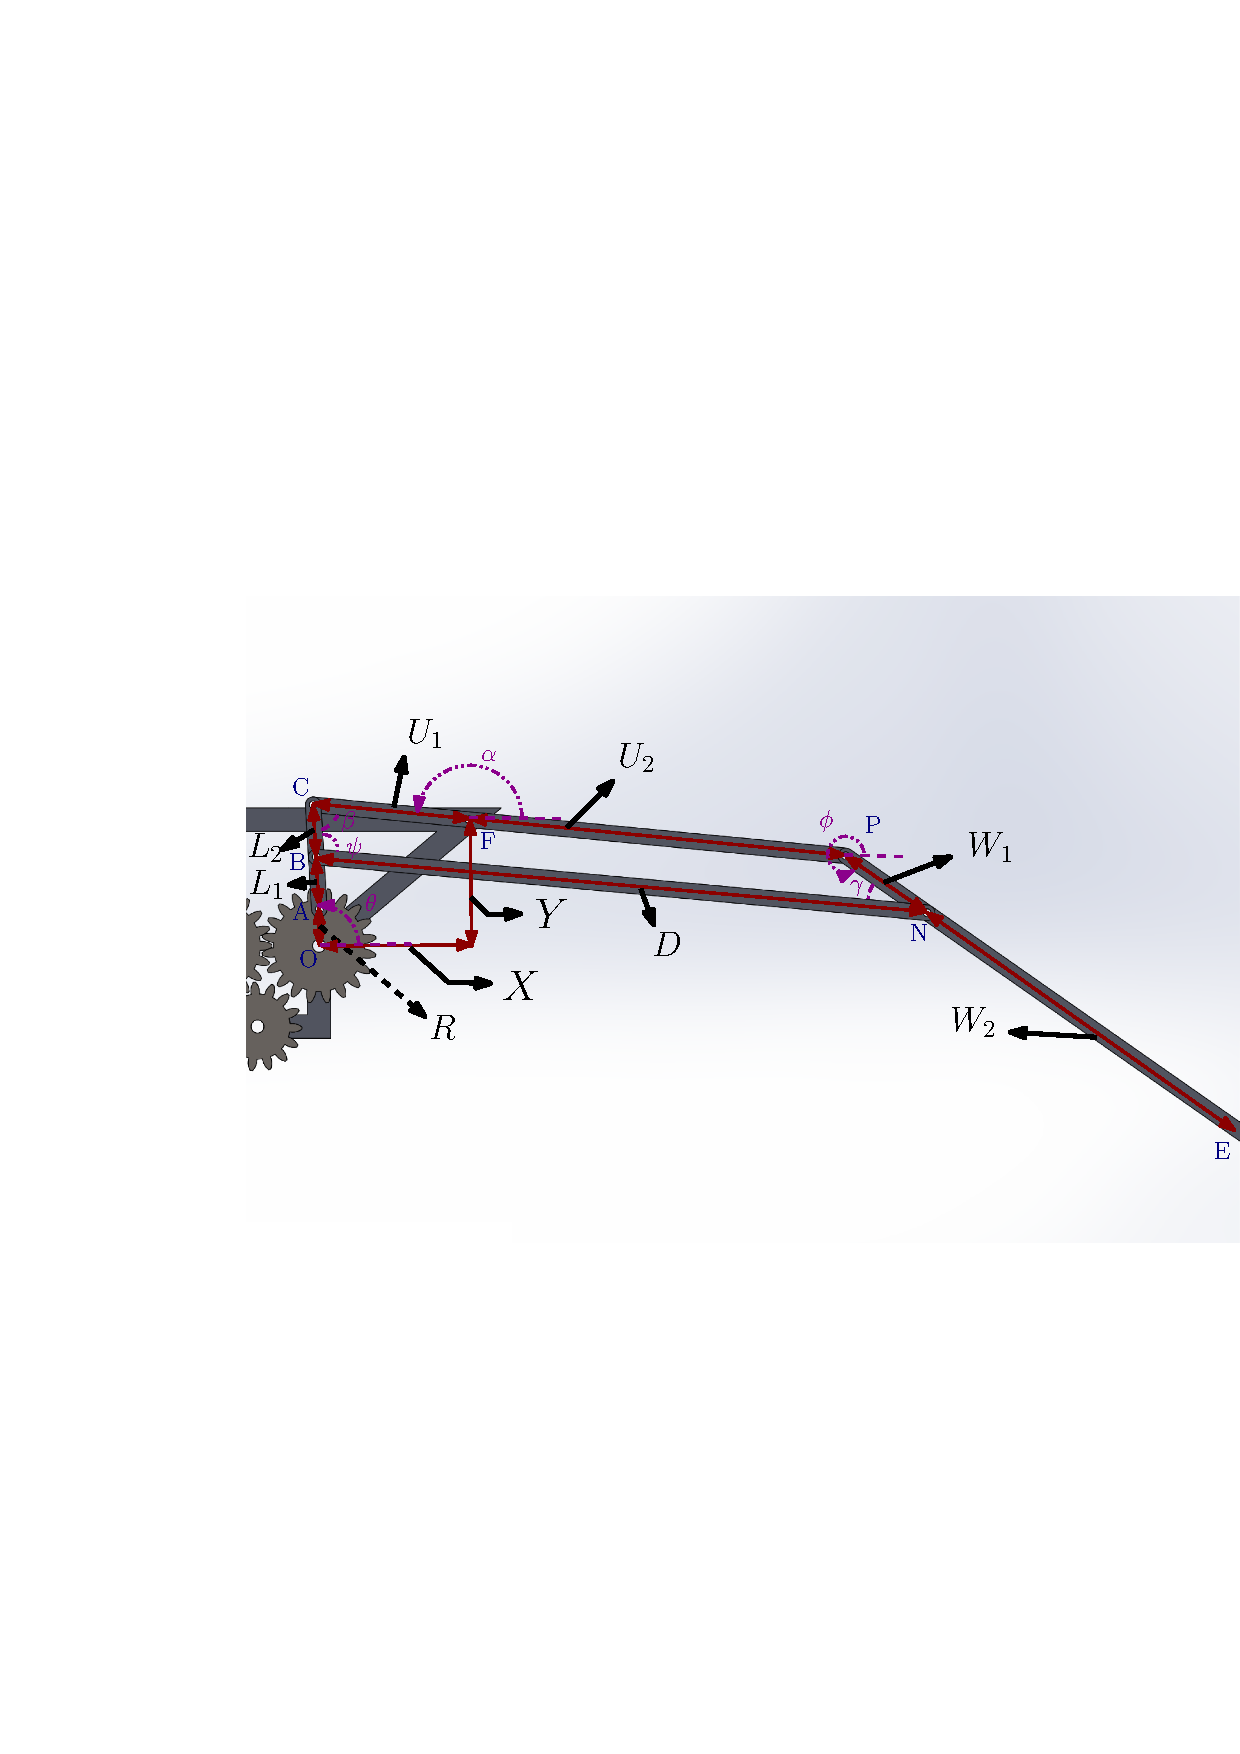
\includegraphics[scale=0.55]{Flapping_Cal_Fig.pdf}
% \end{center}
% \end{block}
% \end{frame}

% \begin{frame}{Wing Flapping}
% \begin{block}{Now we can customize it :)}
% \begin{center}
% 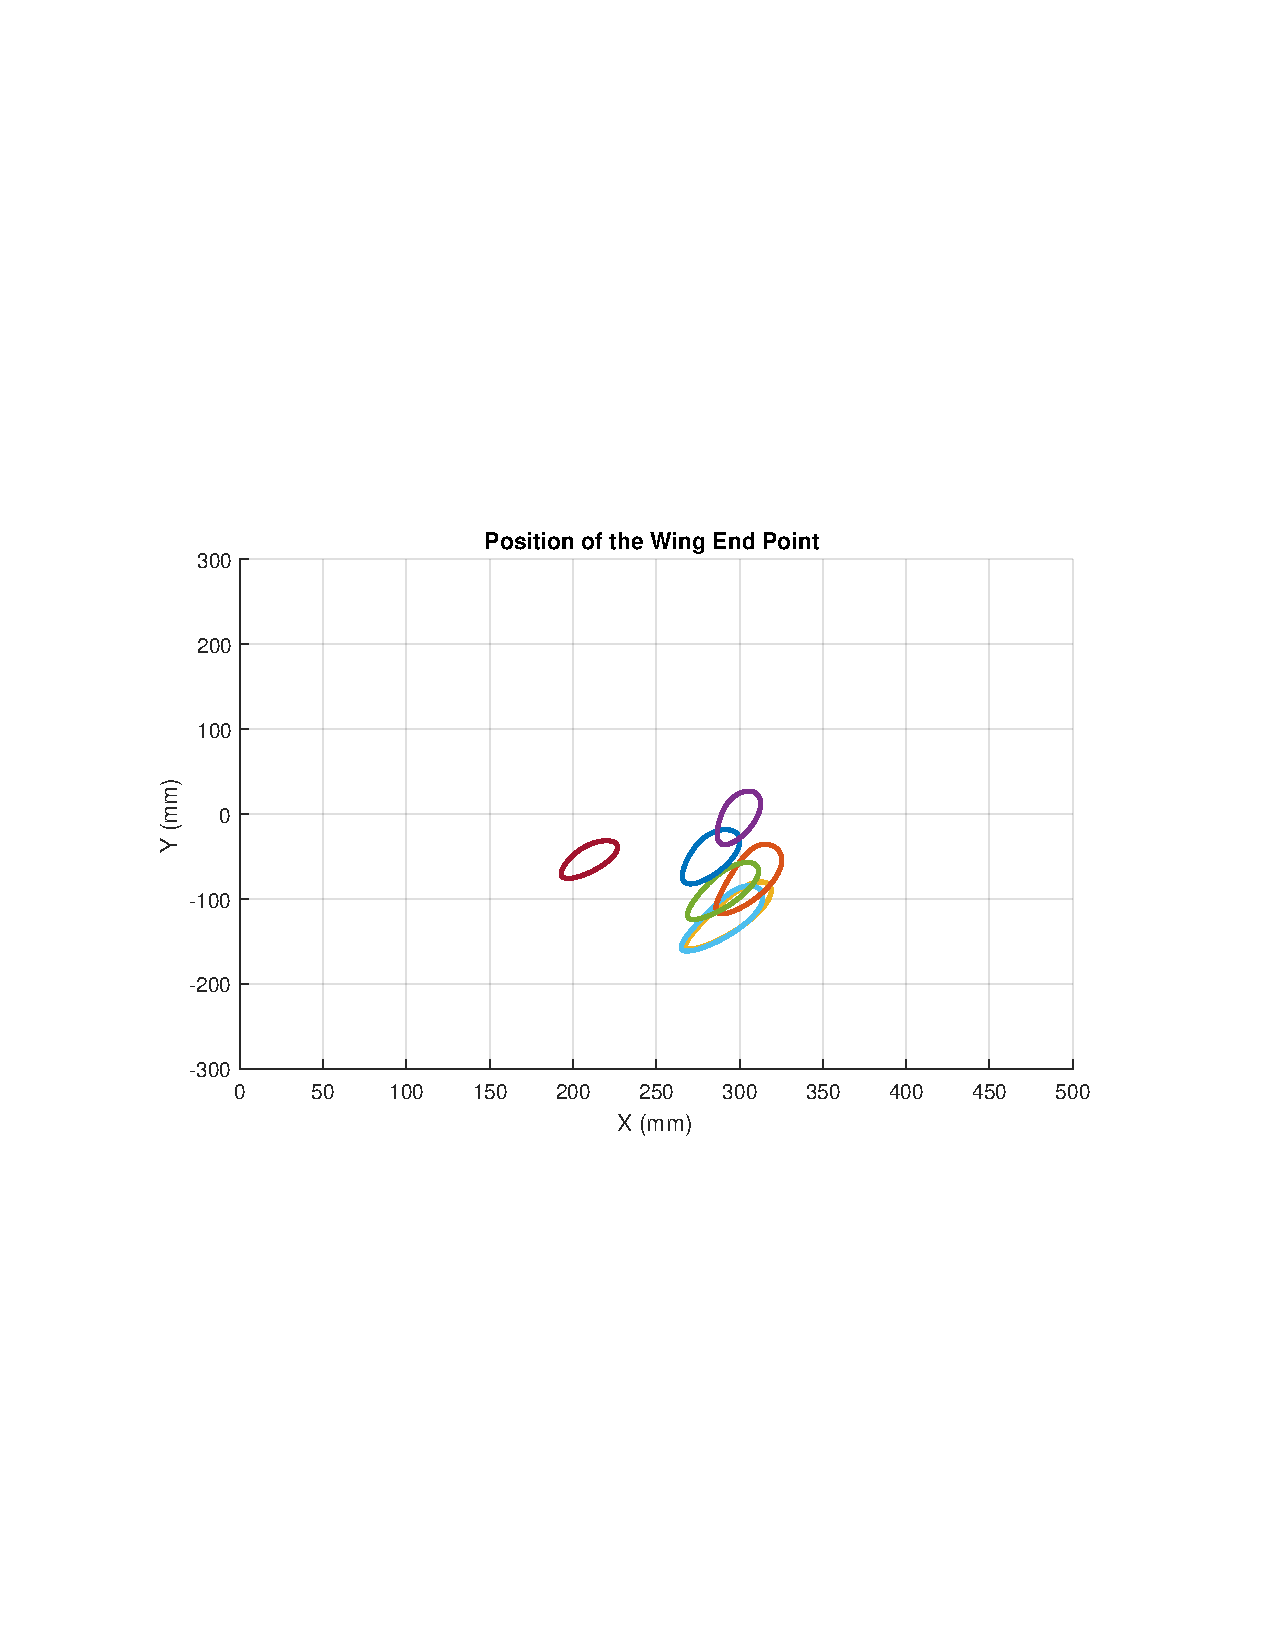
\includegraphics[scale=0.55]{Wing_Fig.pdf}
% \end{center}
% \end{block}
% \end{frame}

% \section{What I'll do?}
% \begin{frame}{What I'll do?}
% \begin{block}{Regarding Paper}
% \begin{itemize}
% \item We compare the Pynamics output
% \item Finishing writing the paper 
% \end{itemize}
% \end{block}
% \begin{block}{Regarding Hydrogel}
% \begin{itemize}
% \item Work on a closed-loop temperature control system for hydrogel
% \end{itemize}
% \end{block}
% \begin{block}{Regarding Summer Robot}
% \begin{itemize}
% \item Make the Dragon-Fly wing 
% \item Write down the FKP 
% \item Customize the design 
% \end{itemize}
% \end{block}
% \end{frame}



% ----------------------- Report of 7 July -------------------------
% ----------------------- Report of 7 July -------------------------
% ----------------------- Report of 7 July -------------------------


\part{Report of 25 August 2017}
% \frame{\partpage}
% \section{What's Done?}

% \begin{frame}{Review Papers}
% \begin{block}{Papers that Focus on Fish Robot:}
% \begin{itemize}
% %\item Model Driven Design for Flexure-Based Microrobots
% \item \href{run:C:/Users/Mohammad/Google Drive/My read papers/4th Presentation/Fish_turning.pdf}{Study on turning performance of a fish robot}
% \vspace{1cm}
% \item \href{run:C:/Users/Mohammad/Google Drive/My read papers/4th Presentation/Parametric.pdf}{Parametric study of the swimming performance of a fish robot propelled by a flexible caudal fin}
% \end{itemize}
% \end{block}
% \end{frame}


% \begin{frame}{finished the 1st Paper - Started to write it}
% \begin{block}{Equilibrium position for the 6-bar mechanism:}
% \begin{itemize}
% \item Pynamics code is being optimized and ready\\
% \textcolor{blue} {Thanks to Dan \& Roozbeh}
% \item Designed and modeled a simple hinge
% \item Have a 6-bar mechanism as case study\\
% Got the data based on Quaternion... We processed it..
% \end{itemize}
% \end{block}
% \end{frame}

% \begin{frame}{finished the 1st Paper - Started to write it}
% \begin{block}{What we have done so far:}
% \begin{table}
% \centering
% \caption{Equilibrium Angles (deg).}
%  \begin{tabular}{>{\centering\arraybackslash}m{2.5cm} >{\centering\arraybackslash}m{3.5cm} >{\centering\arraybackslash}m{3.5cm}}
% \hline
% Angle Number
% & 
% Pynamics 
% &
% Experimental Data
% \\ \hline
% 1
% &
% 12.7
% &
% 22.9
% \\ \hline
% 2
% &
% 0.41
% &
% 6.53
% \\ \hline
% 3
% &
% 31.81
% &
% 28.8
% \\ \hline
% 4
% &
% -38.34
% &
% -42.3
% \\ \hline
% 5
% &
% -9.16
% &
% -9.23
% \\ \hline
% 6
% &
% -9.46
% &
% -9.53
% \\ \hline
% \end{tabular}
% \end{table}
% \end{block}
% \end{frame}


% \begin{frame}{SRP Fish}
% \begin{block}{Making sub-projects}
% \begin{itemize}
% \item Designing Test bed
% \item Design optimization of tail fin
% \item Design optimization of side fins
% \item Design Grasping fins
% \item Identification of Fish movement in water 
% \item Control of the fish moving forward
% \item Control of the fish stabilization
% \item Adding Knitting-brushing modules
% \item Control the fish under working disturbance
% \end{itemize}
% \end{block}
% \end{frame}

% \begin{frame}{Test setup design}
% \begin{block}{Use force acceleration instead of movement}
% \begin{center}
% 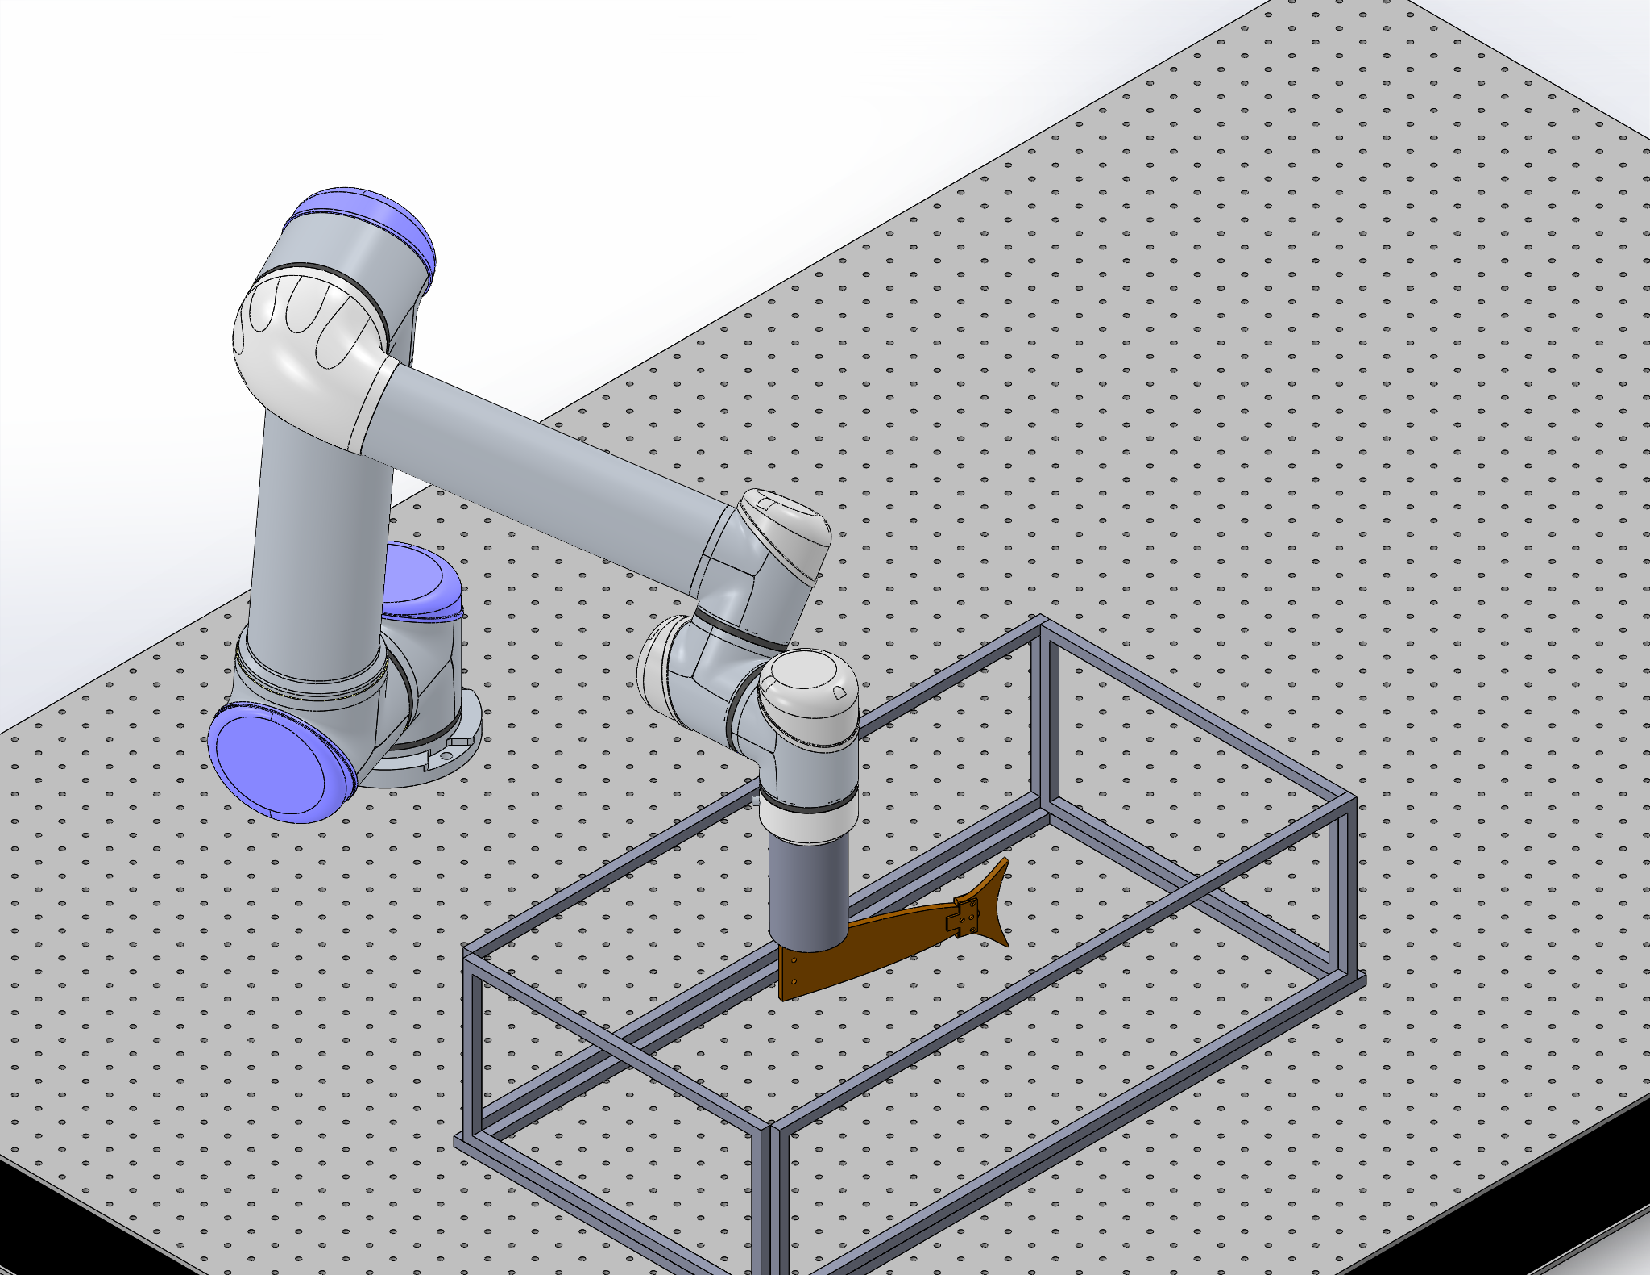
\includegraphics[scale=0.27]{Test_Bed.pdf}
% \end{center}
% \end{block}
% \end{frame}

% \begin{frame}{Designing the first prototype}
% \begin{block}{First prototype design}
% \begin{center}
% 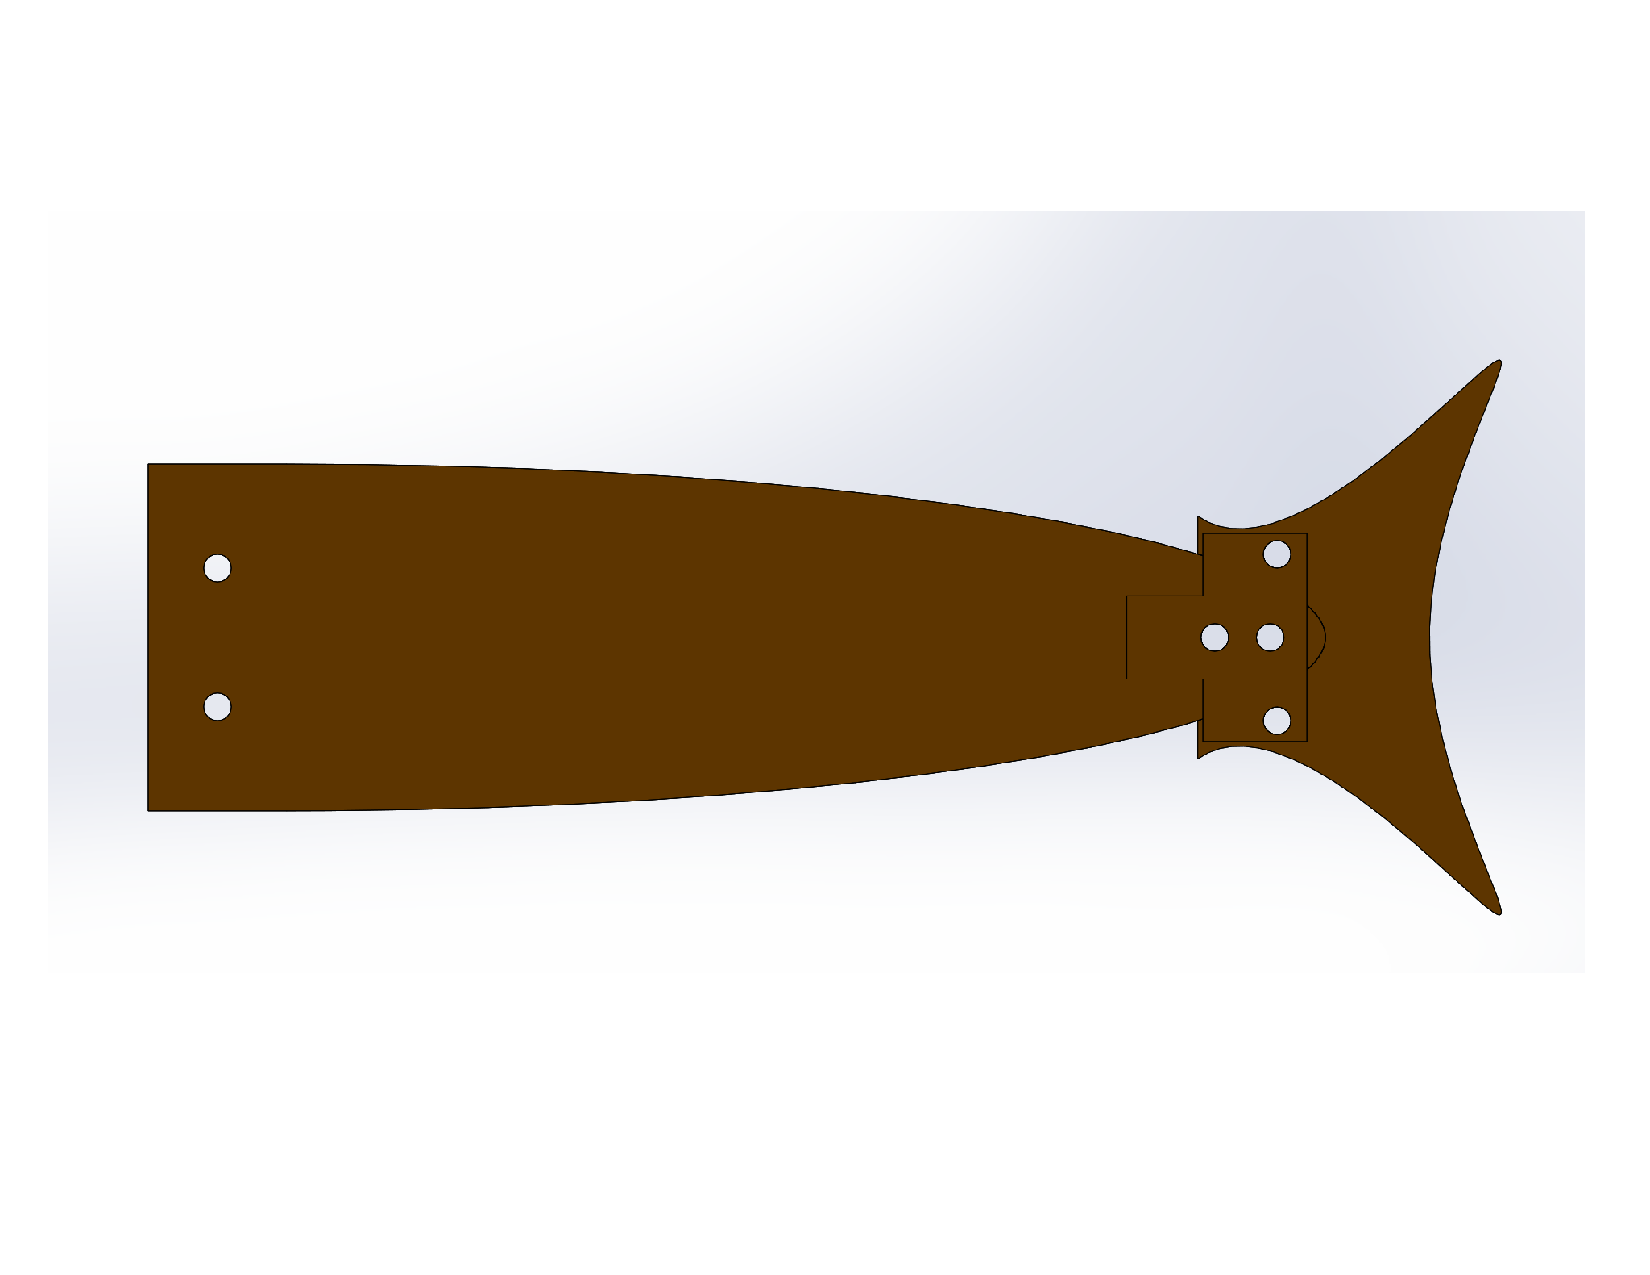
\includegraphics[scale=0.42]{First_Prototype.PDF}
% \end{center}
% \end{block}
% \end{frame}

% \begin{frame}{Built the first prototype}
% \begin{block}{First prototype tail is built}
% \begin{center}
% 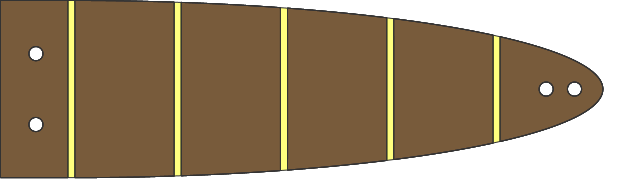
\includegraphics[scale=0.5]{Tail1.png}
% \end{center}
% \end{block}
% \end{frame}

% \begin{frame}{Built the first prototype}
% \begin{block}{First prototype tail is built}
% \begin{center}
% 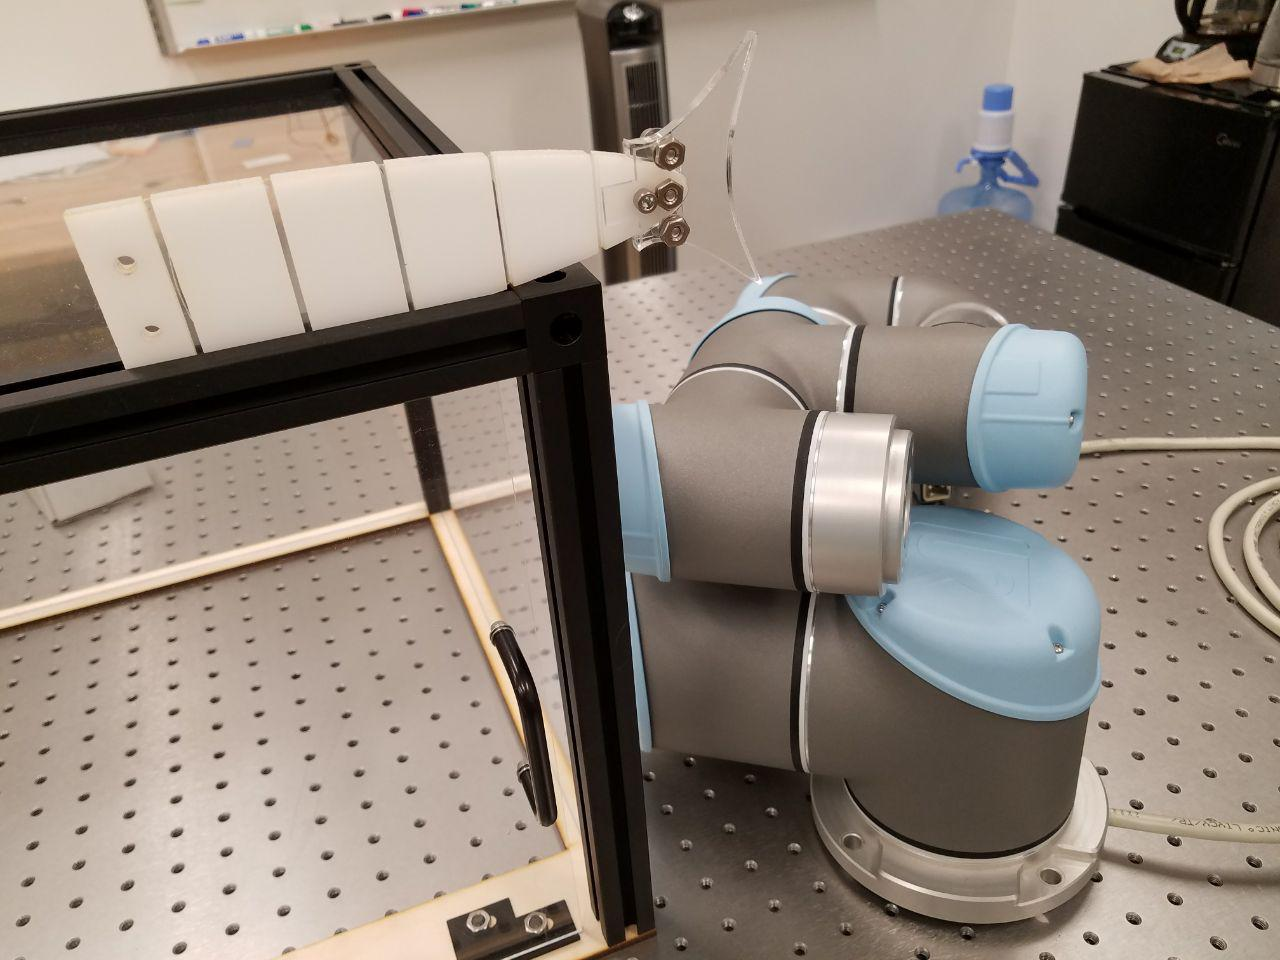
\includegraphics[scale=0.24]{Fish_tail1.jpg}
% \end{center}
% \end{block}
% \end{frame}

% \section*{What I'll do...}

% \begin{frame}{What I'll do...}
% \begin{block}{paper}
% \begin{itemize}
% \item Continue writing the paper
% \end{itemize}
% \end{block}
% \end{frame}

% \begin{frame}{What I'll do...}
% \begin{block}{SRP fish}
% \begin{itemize}
% \item Design and build the connection between the force sensor and fish
% \item Find the proper waterproof servo
% \item Design the connector between the servo and the tail
% \item Design the body of the fish
% \end{itemize}
% \end{block}
% \end{frame}

% \begin{frame}{What I need help with...}
% \begin{block}{SRP fish}
% Let's go over the papers one more time  
% \begin{itemize}
% \item \Large We have problem with water current cause by flapping \normalsize
% \begin{enumerate}
% \item  Identify the water current and waves 
% \item change it to movement $\Rightarrow$  Study "Moving forward range" and "How much it diverges from straight line".
% \item Find or Design a water tunnel in order to produce a constant current.
% \end{enumerate}
% \item \Large Tail Moving $\&$ Flapping Fin \LARGE VS \Large Tail Flapping 
% \end{itemize}
% \end{block}
% \end{frame}

\part{Report of 29 September 2017 }
\frame{\partpage}
\section{What's Done?}

\begin{frame}{Review Papers}
\begin{block}{Papers that Focus on Fish Robot:}
\begin{itemize}
%\item Model Driven Design for Flexure-Based Microrobots
\item \href{run:C:/Users/Mohammad/Google Drive/My read papers/5th Presentation/Miniature_Fish.pdf}{Infiltrating the zebrafish swarm: design, implementation and experimental tests of a miniature robotic fish lure for fish-robot interaction studies}
\vspace{0.7cm}
\item \href{run:C:/Users/Mohammad/Google Drive/My read papers/5th Presentation/fins_for_fish.pdf}{Modelling and parametric study of modular undulating fin rays for fish robots}

\vspace{0.7cm}
\item \href{run:C:/Users/Mohammad/Google Drive/My read papers/5th Presentation/Book_Model_Test.pdf
}{Marine Hydrodynamics, by: Newman}
\end{itemize}
\end{block}
\end{frame}





\begin{frame}{SRP Fish}
\begin{block}{Making sub-projects}
\begin{itemize}
\color{blue}
\item Propose initial prototypes
\item Designing Test bed
\item Design optimization of tail
\item Design optimization of side fins
\item Control of the fish stabilization
\color{black}
\item Identification of Fish movement in water 
\item Control of the fish moving forward
\item Design Grasping fins
\item Adding Knitting-brushing modules
\item Fish under working disturbance
\end{itemize}
\end{block}
\end{frame}

% \begin{frame}{Designing the first prototype}
% \begin{block}{First prototype design}
% \begin{center}
% 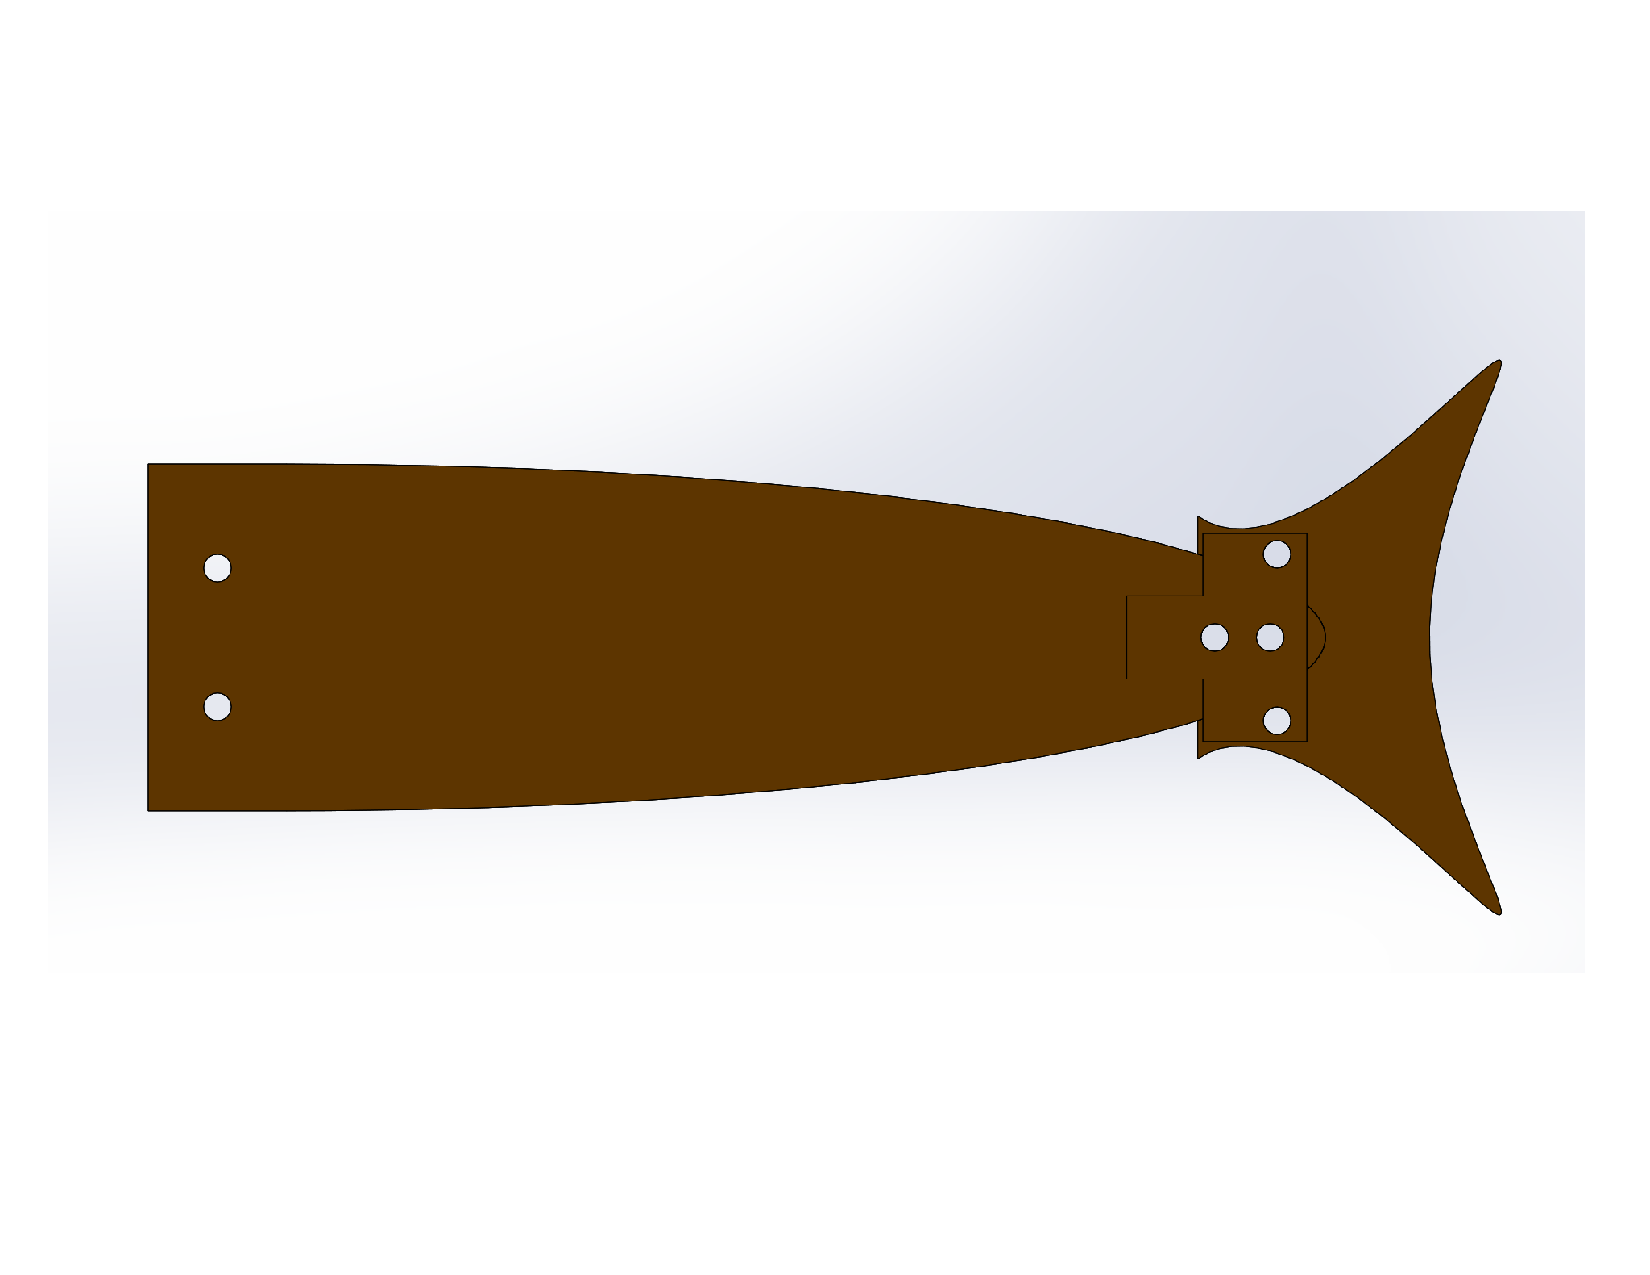
\includegraphics[scale=0.42]{First_Prototype.PDF}
% \end{center}
% \end{block}
% \end{frame}

% \begin{frame}{Designing the first prototype}
% \begin{block}{First prototype tail is built}
% \begin{center}
% 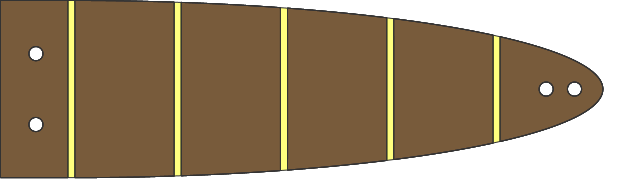
\includegraphics[scale=0.5]{Tail1.png}
% \end{center}
% \end{block}
% \end{frame}

\begin{frame}{Building initial prototypes}
\begin{block}{First prototype}
\begin{center}
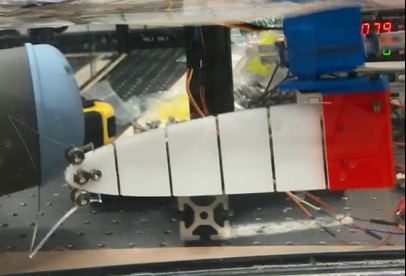
\includegraphics[scale=0.7]{1st_PR.png}
\end{center}
\end{block}
\end{frame}

\begin{frame}{Building initial prototypes}
\begin{block}{Second prototype}
\begin{center}
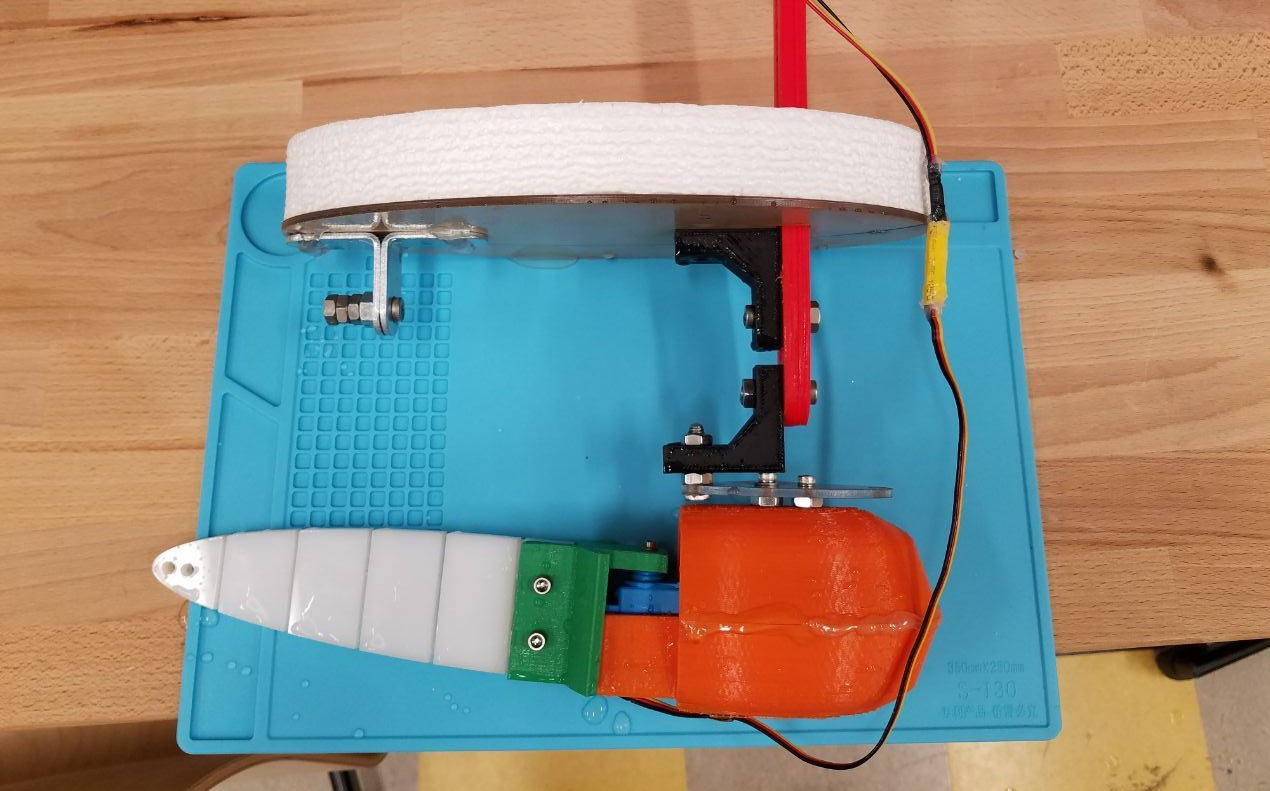
\includegraphics[scale=0.27]{2nd_PR.jpg}
\end{center}
\end{block}
\end{frame}


\begin{frame}{Test setup design}
\begin{block}{Use force acceleration instead of movement \color{red} \huge ? \normalsize \color{black}}
\begin{center}
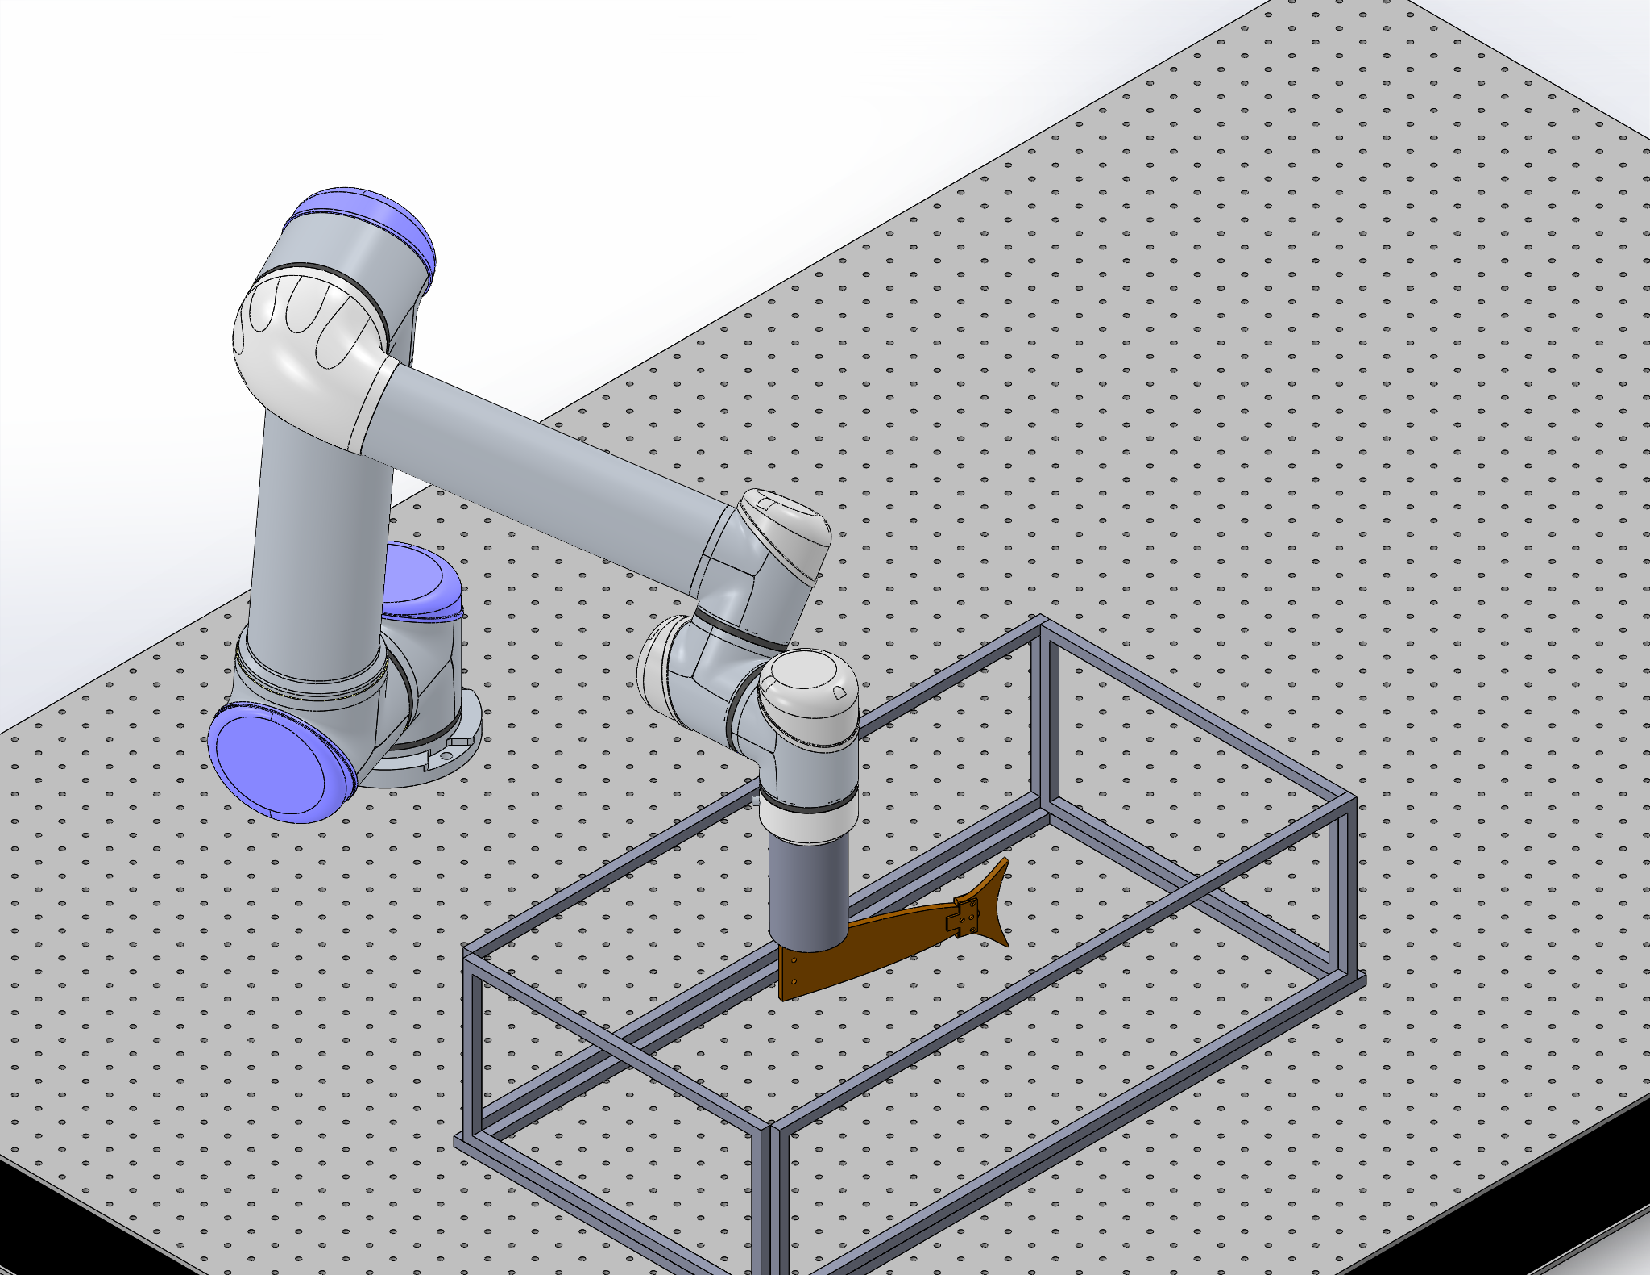
\includegraphics[scale=0.27]{Test_Bed.pdf}
\end{center}
\end{block}
\end{frame}

\begin{frame}{Design optimization of tail}
\begin{block}{How many? \qquad\qquad Length? \qquad\qquad Width?}
\begin{center}
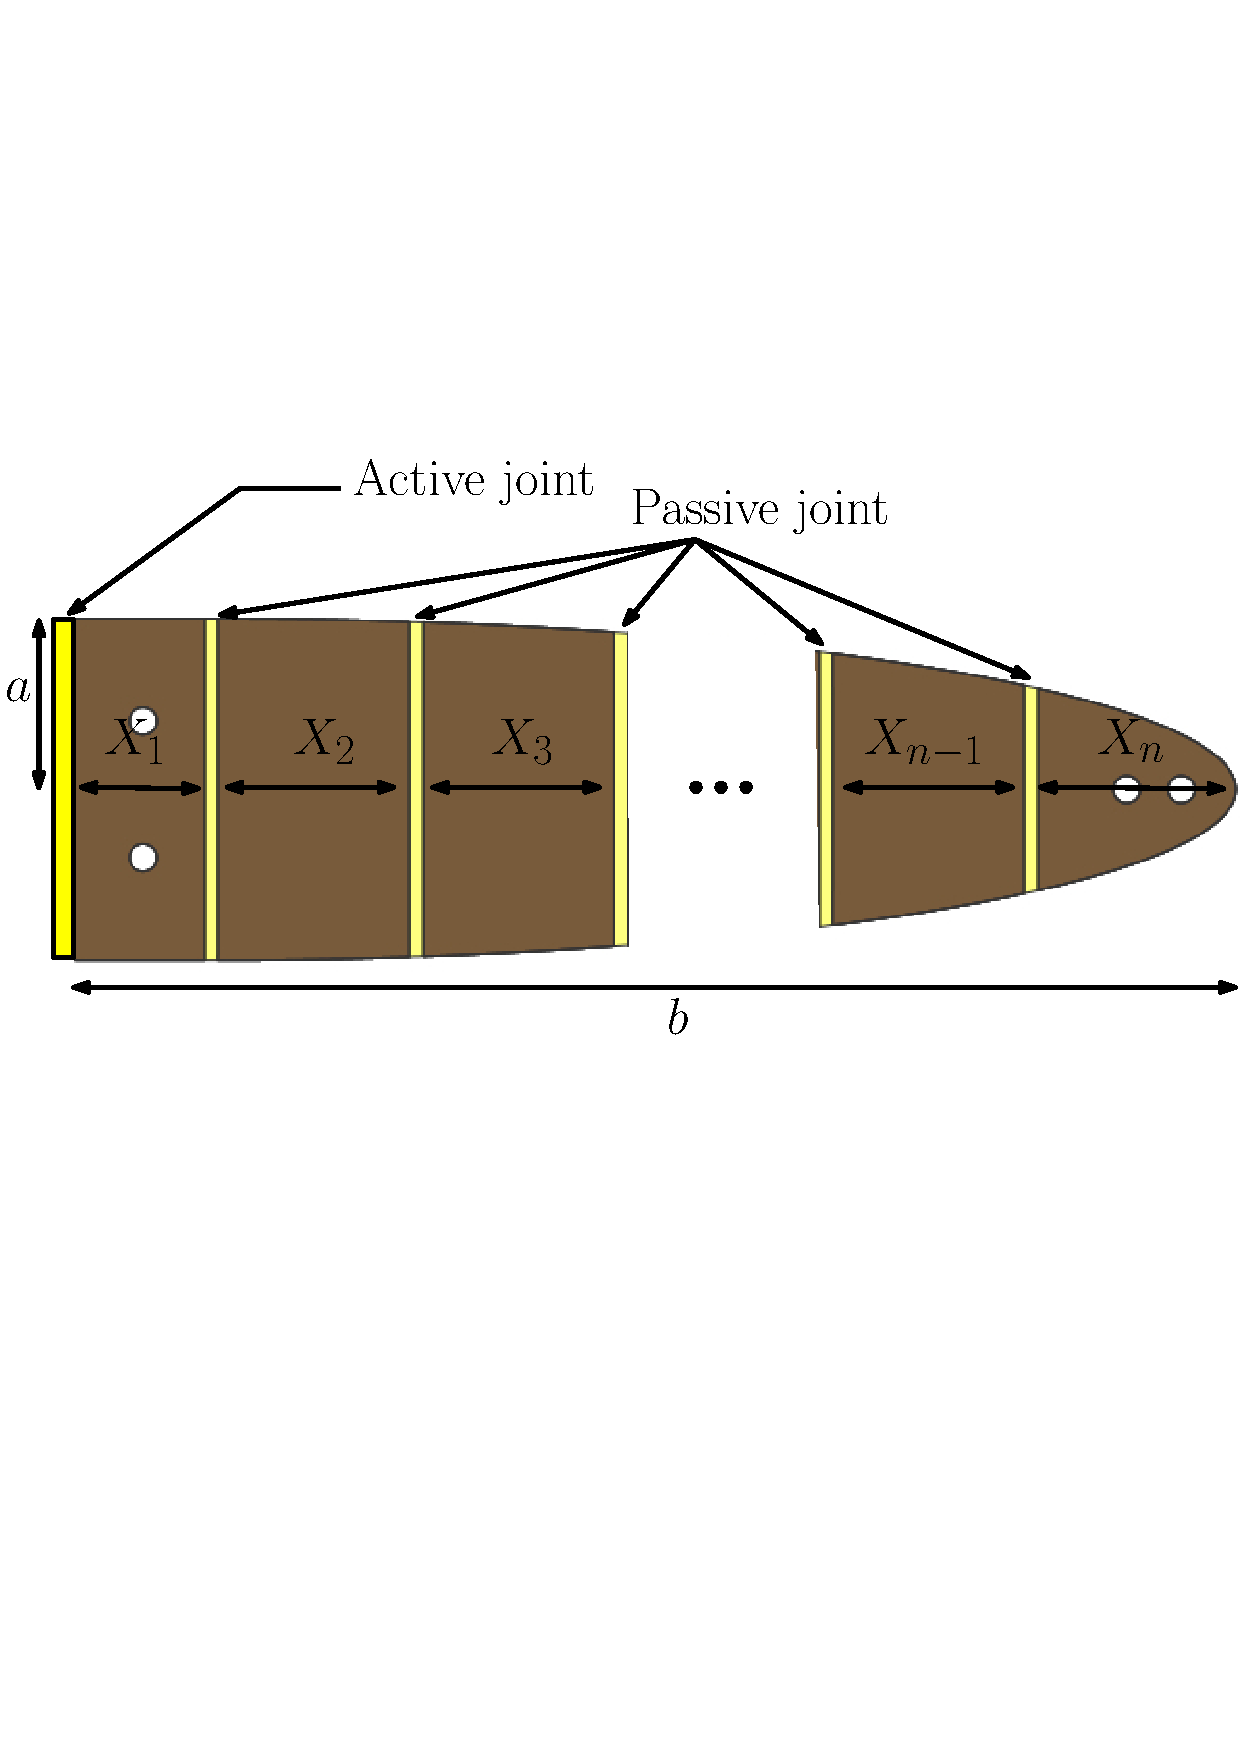
\includegraphics[scale=0.45]{Tail1.pdf}
\begin{equation*}
\textbf{Ellipse Function:}  \dfrac{x^2}{b^2} + \dfrac{y^2}{a^2} = 1
\end{equation*}
\end{center}
\end{block}
\end{frame}

\begin{frame}{Design optimization of side fin}
\begin{block}{5bar design angles? \qquad \qquad Length?}
\begin{center}
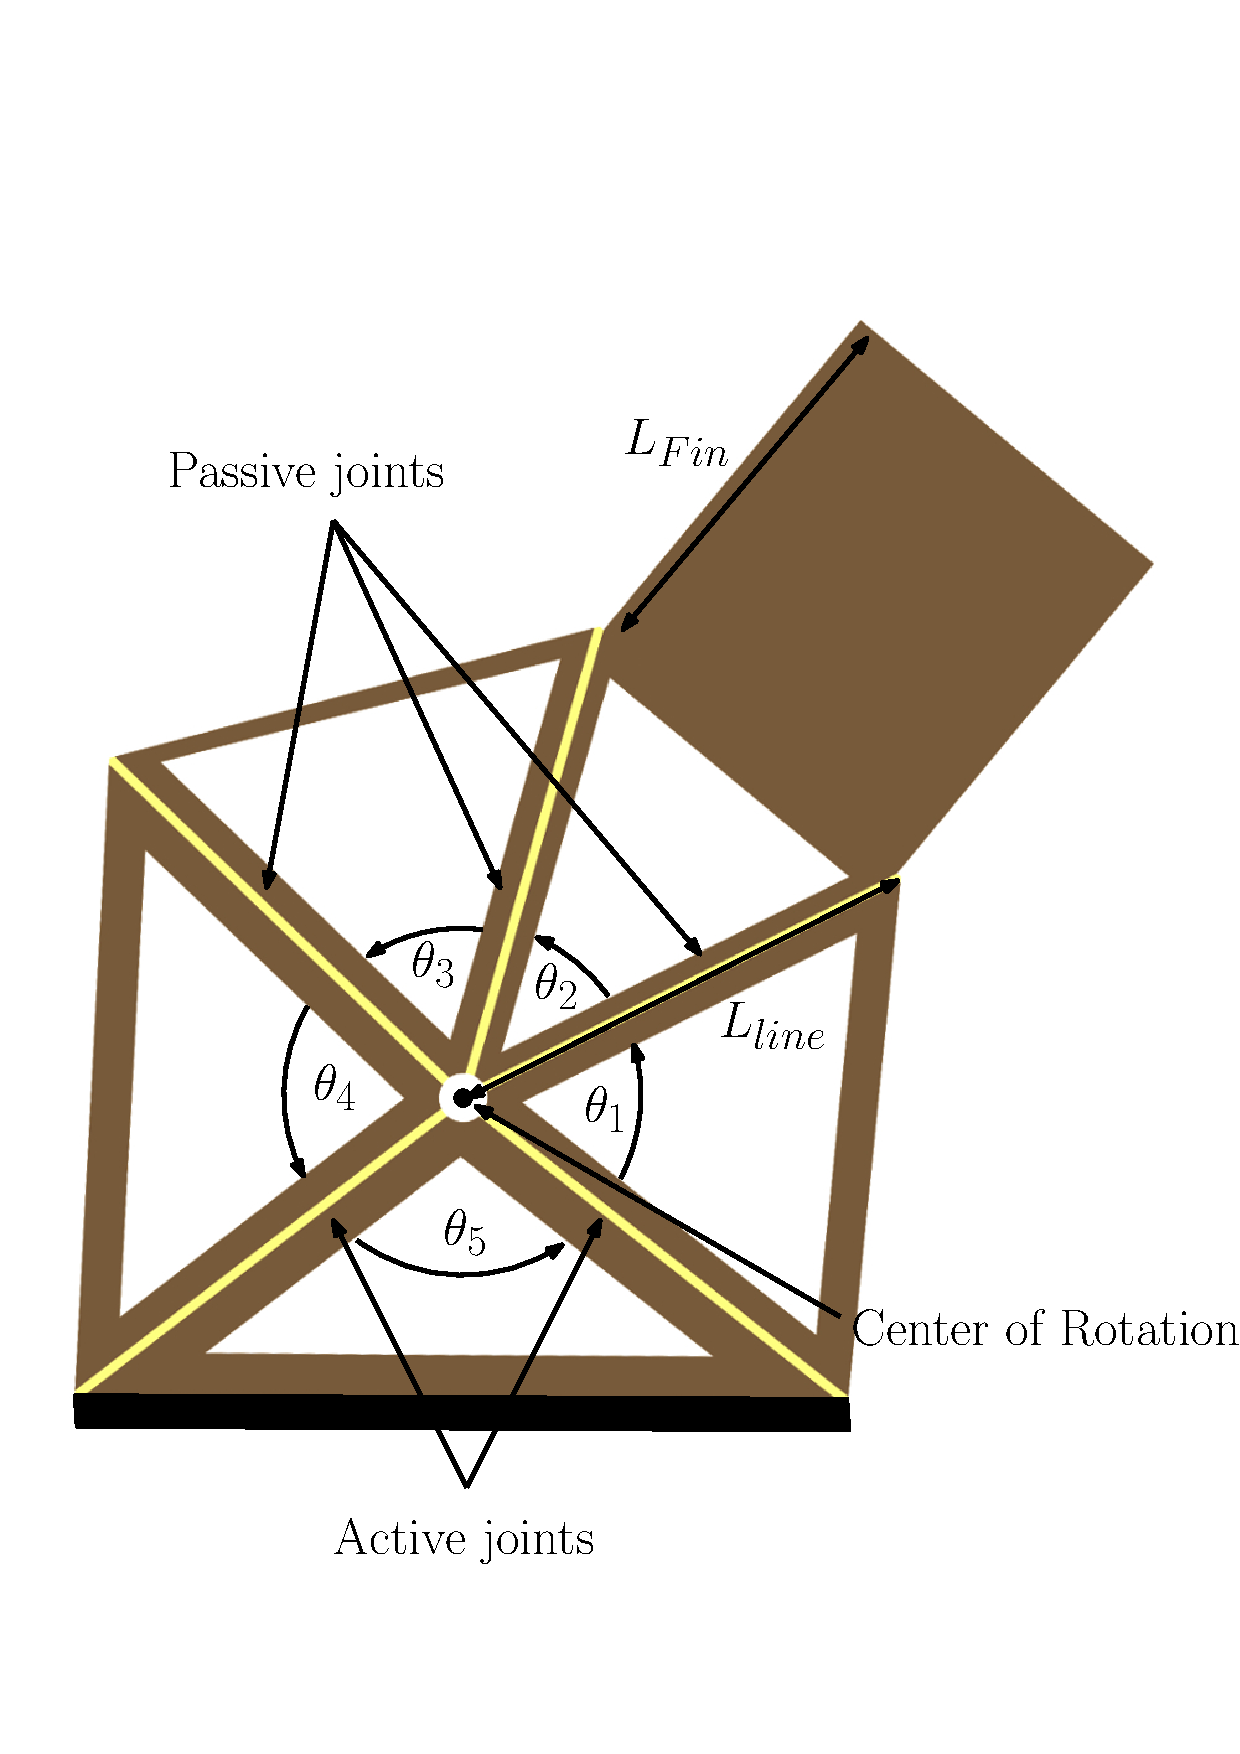
\includegraphics[scale=0.27]{5bar_Fin.pdf}
\end{center}
\end{block}
\end{frame}

\begin{frame}{Control of the fish stabilization}
\begin{block}{Idea}
\begin{center}
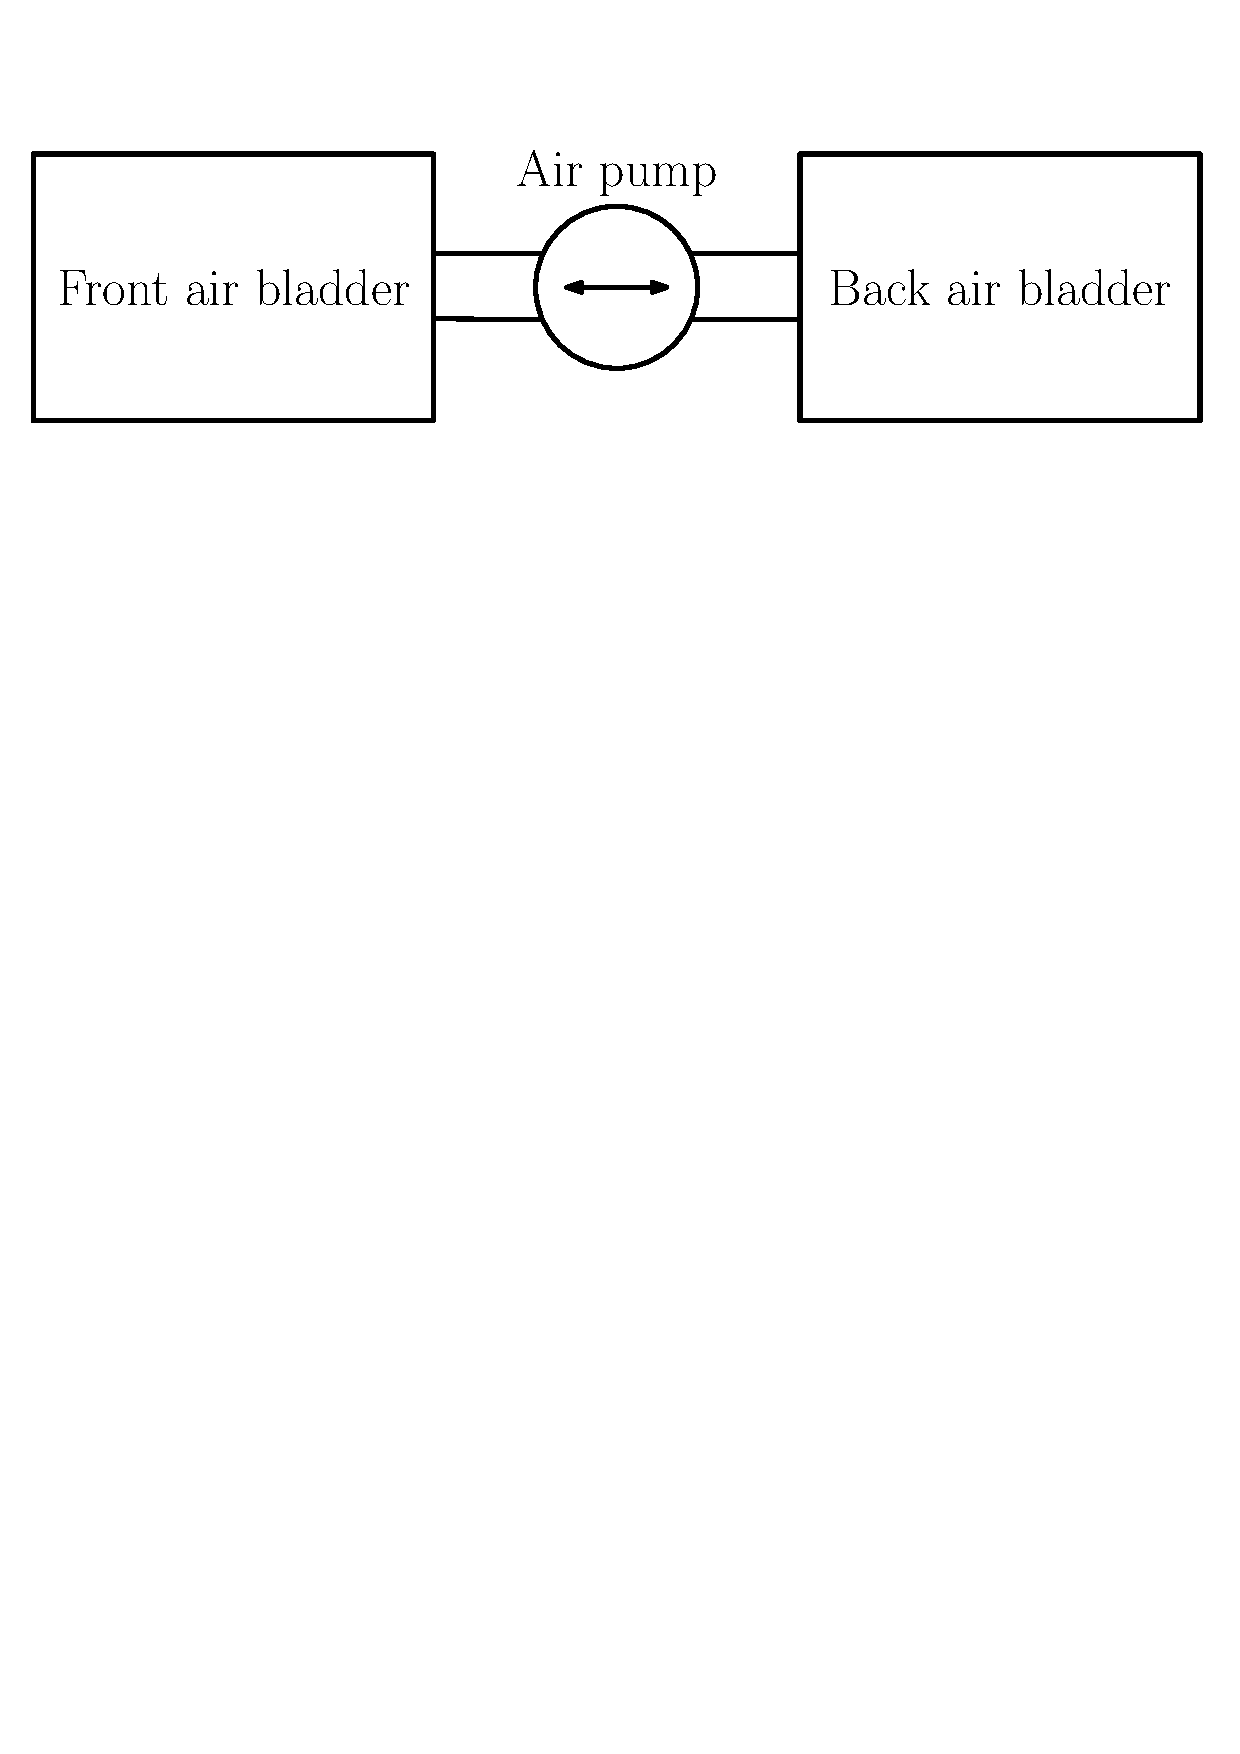
\includegraphics[scale=0.5]{Bladder_Idea.pdf}
\end{center}
\end{block}
\end{frame}


\section*{What I'll do...}

\begin{frame}{What I'll do...}
\begin{block}{SRP fish}
\begin{itemize}
\item Get data from the fish
\item Find drag \& lifting force model
\item Get the symbolic formulation out of Pynamics\color{red}\large ?\normalsize \color{black}
\end{itemize}
\end{block}
\end{frame}


\end{document}

